% Abyss technical report (English): running DeepSeek-V4.1-Flash in tiers on two GPUs
% Build: tectonic -X compile report-en.tex (fonts: Palatino, Helvetica Neue, Menlo and, for the full-width characters of
% DeepSeek control tokens such as <｜User｜>, Songti SC, all shipped with macOS)
\documentclass[11pt,a4paper]{article}

\usepackage[a4paper,top=2.6cm,bottom=2.6cm,left=2.7cm,right=2.7cm]{geometry}
\usepackage{fontspec}
\usepackage{xeCJK}
\setmainfont{Palatino}
\setsansfont{Helvetica Neue}
\setmonofont{Menlo}[Scale=0.82]
\setCJKmainfont[BoldFont={Songti SC Bold}]{Songti SC}
\setCJKsansfont{Songti SC}
\setCJKmonofont{Songti SC}
\linespread{1.15}
\setlength{\emergencystretch}{2em}

\usepackage{amsmath}
\usepackage{graphicx}
\usepackage{booktabs}
\usepackage{tabularx}
\usepackage{array}
\usepackage{multirow}
\usepackage{xcolor}
\usepackage{enumitem}
\usepackage{caption}
\usepackage{subcaption}
\usepackage{tikz}
\usepackage{pgfplots}
\usetikzlibrary{positioning,arrows.meta,calc}
\pgfplotsset{compat=1.18}
\usepackage{hyperref}
\hypersetup{colorlinks=true,linkcolor=dsblue,citecolor=dsblue,urlcolor=dsblue}

\definecolor{dsblue}{HTML}{4D6BFE}
\definecolor{dsviolet}{HTML}{8E7CF0}
\definecolor{dslight}{HTML}{C9D3FF}
\definecolor{dsgray}{HTML}{B8BCC8}
\definecolor{dsdark}{HTML}{1E2A5A}
\definecolor{dsorange}{HTML}{F29A4A}

\DeclareCaptionLabelSeparator{bar}{\ |\ }
\captionsetup{labelsep=bar,font=small,justification=justified,singlelinecheck=false}
\captionsetup[sub]{labelformat=parens,labelsep=space,justification=centering}
\renewcommand{\figurename}{Figure}
\renewcommand{\tablename}{Table}
\renewcommand{\contentsname}{Contents}
\renewcommand{\refname}{References}
\renewcommand{\appendixname}{Appendix}

\setlist{itemsep=0.2em,topsep=0.4em}
\newcommand{\code}[1]{\texttt{#1}}
\newcommand{\tps}{tok/s}
\newcommand{\ctok}[1]{\mbox{\xeCJKsetup{CJKecglue={}}\code{#1}}}

\pgfplotsset{
  abyss/.style={
    axis lines*=left,
    ymajorgrids,
    grid style={dsgray!40},
    tick label style={font=\footnotesize},
    label style={font=\footnotesize},
    legend style={font=\footnotesize,draw=none,fill=none},
    every axis plot/.append style={line width=0.6pt},
  },
}
\begin{document}

% ---------------------------------------------------------------- title page
\thispagestyle{empty}
\noindent

\begin{tikzpicture}[baseline=(t.base)]
  \fill[dsblue] (0,0) rectangle (0.62,0.62);
  \draw[white,line width=1.4pt,line cap=round] (0.10,0.36) .. controls (0.20,0.48) and (0.26,0.48) .. (0.31,0.36) .. controls (0.36,0.24) and (0.42,0.24) .. (0.52,0.36);
  \draw[white!70!dsblue,line width=1.1pt,line cap=round] (0.10,0.20) .. controls (0.20,0.30) and (0.26,0.30) .. (0.31,0.20) .. controls (0.36,0.10) and (0.42,0.10) .. (0.52,0.20);
  \node[anchor=west,inner sep=0] (t) at (0.80,0.31) {\sffamily\bfseries\Large\color{dsblue}abyss};
\end{tikzpicture}

\vspace{0.6em}
\begin{center}
  {\LARGE\bfseries Abyss: Running DeepSeek-V4.1-Flash\\[0.25em] in Tiers on Two GPUs}\\[1.0em]
  {\large Abyss}\\[0.2em]
  {\small November 2026}
\end{center}

\vspace{0.4em}
\begin{center}{\large\bfseries Abstract}\end{center}
\vspace{-0.3em}
\noindent
Long-context agents have moved the pressure in inference from compute to VRAM, host memory and PCIe. DeepSeek-V4.1-Flash has 763B parameters in total and about 474 GiB of native weights, more than the entire capacity of a two-GPU workstation (2 × RTX PRO 6000 Max-Q with 191 GiB of VRAM combined; 192 GB of host memory). We implemented Abyss, a tiered inference scheduler, on mx-llama.cpp: the experts of the encoder layers stay resident in VRAM, the experts of the decoder's last 18 layers are kept in host memory and served jointly by an expert cache on the GPU and by the CPU, and the large Engram tables stay on NVMe. Keeping native MXFP4 precision (each change differs from the version before it by no more than the numerical floor), we wrote more than forty patches around the model's encoder-decoder structure (CED), compressed attention and sparse indexer. On the prefill side, CED-aware prefill has the decoder layers compute only the tokens that later tokens can still see; together with the official sparse indexer, Engram prefetch, the big-batch split in prefill, the one-pass prompt tail and the two-GPU pipeline for long prompts, it brought a 48K-token prompt from 135 s down to about 14 s (about 3,400 \tps{}), and the prefill of each later turn in a multi-turn agent session from 5.7--7.2 s down to about 2 s. On the decode side, the GPU expert cache, heat-based admission of misses with the rest handed to the CPU, expert deferral (experts computed on the CPU are added back to the residual one layer later), the cache's admission gate, small-kernel fusion, computing half of the output head on each GPU and other changes raised single-stream decode from 14.1 \tps{} to about 52 \tps{} in an append-only multi-turn session (96K context; about 50 \tps{} per request in production); the context grew from 128K to 192K, and memory went from 3600 to 6000 MT/s. With the same weights and the same launch parameters, upstream llama.cpp decodes about 20\% slower and takes more than 5 times as long to prefill long prompts; subsets run with the data and clients of three public agent benchmarks (MLPerf Agentic Inference, InferenceX AgentX, TraceLab) lead to the same conclusion (none of them are official results): the same work takes us about half as long as it takes upstream, and only TraceLab's median time to first token is worse than upstream's, because of one checkpoint trade-off. On the serving side, we rewrote the chat template after the official \code{encoding.py}, encoded control-token text in requests by the rules of the official Recipe, stopped recomputing the previous turn's answer every turn, and fixed several defects that real Codex and Hermes workloads exposed; the weights were switched to the 1017 version that DeepSeek released on October 17 (converted ourselves, 3.4\% lower PPL). We also record our evaluation methods (two tiers of numerical floor, cross-checks against the official implementation, decode-path PPL, speed tests with fixed seeds), two measurement pitfalls that led our conclusions astray (generating from the same prompt again inflates decode speed, and node-level tracing in nsys inflates the cost of CUDA graph launches), and the paths we implemented or measured but did not adopt: expert prefetch, DSpark speculative decoding, one fewer expert per token, a Q8\_0 output head and tensor parallelism for layers 0--19.

\vspace{0.2em}
\begin{figure}[!h]
  \centering
  \begin{subfigure}[b]{\textwidth}
    \centering
    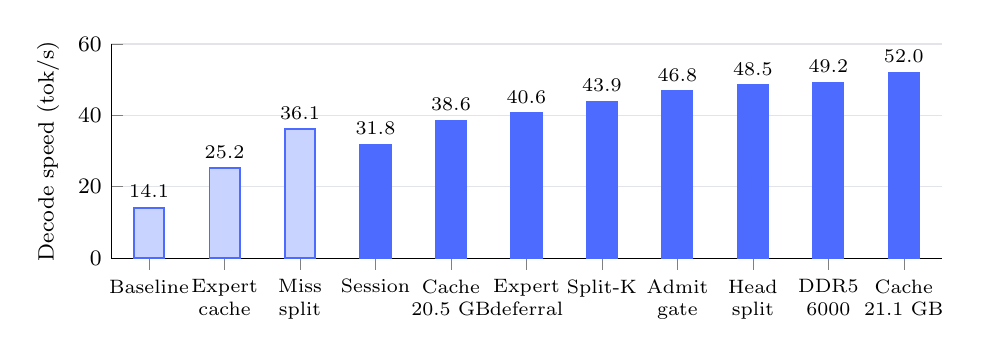
\begin{tikzpicture}
      \begin{axis}[abyss,
        width=\linewidth, height=4.3cm,
        ybar, bar width=11pt, ymin=0, ymax=60,
        ylabel={Decode speed (\tps)},
        xtick={1,2,3,4,5,6,7,8,9,10,11},
        xticklabels={Baseline, Expert\\cache, Miss\\split, Session, Cache\\20.5 GB, Expert\\deferral, Split-K, Admit\\gate, Head\\split, DDR5\\6000, Cache\\21.1 GB},
        xticklabel style={font=\scriptsize,align=center,text width=1.2cm},
        nodes near coords={\pgfmathprintnumber[fixed,fixed zerofill,precision=1]{\pgfplotspointmeta}},
        nodes near coords style={font=\scriptsize},
        enlarge x limits=0.05]
        \addplot[fill=dslight,draw=dsblue,bar shift=0pt] coordinates {(1,14.1) (2,25.2) (3,36.1)};
        \addplot[fill=dsblue,draw=dsblue,bar shift=0pt] coordinates {(4,31.8) (5,38.6) (6,40.6) (7,43.9) (8,46.8) (9,48.5) (10,49.2) (11,52.0)};
      \end{axis}
    \end{tikzpicture}
    \caption{}
  \end{subfigure}

  \vspace{0.4em}
  \begin{subfigure}[b]{0.66\textwidth}
    \centering
    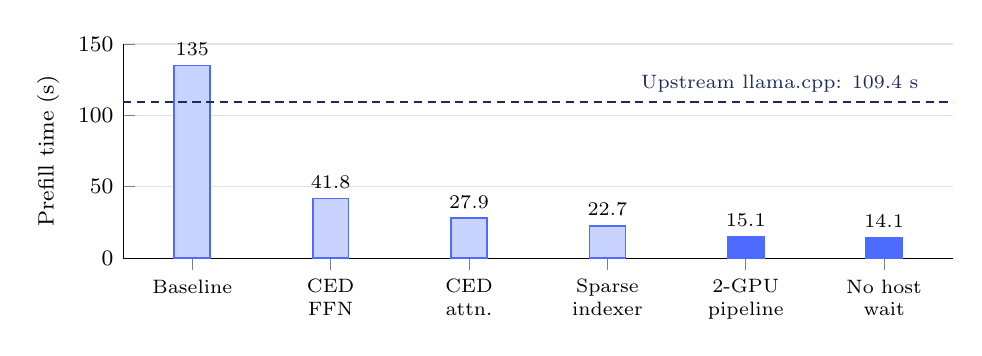
\begin{tikzpicture}
      \begin{axis}[abyss,
        width=\linewidth, height=4.3cm,
        ybar, bar width=13pt, ymin=0, ymax=150,
        ylabel={Prefill time (s)},
        xtick={1,2,3,4,5,6},
        xticklabels={Baseline, CED\\FFN, CED\\attn., Sparse\\indexer, 2-GPU\\pipeline, No host\\wait},
        xticklabel style={font=\scriptsize,align=center,text width=1.1cm},
        nodes near coords, nodes near coords style={font=\scriptsize},
        enlarge x limits=0.1]
        \addplot[fill=dslight,draw=dsblue,bar shift=0pt] coordinates {(1,135) (2,41.8) (3,27.9) (4,22.7)};
        \addplot[fill=dsblue,draw=dsblue,bar shift=0pt] coordinates {(5,15.1) (6,14.1)};
        \draw[dsdark, densely dashed, line width=0.6pt] ({rel axis cs:0,0} |- {axis cs:1,109.4}) -- ({rel axis cs:1,0} |- {axis cs:1,109.4}) node[pos=0.97, above, font=\scriptsize, anchor=south east] {Upstream llama.cpp: 109.4 s};
      \end{axis}
    \end{tikzpicture}
    \caption{}
  \end{subfigure}
  \caption{(a) Single-stream decode speed as the optimizations are added one after another (Section~\ref{sec:decode}). The 3 light bars are at 48K context, generating from the same prompt a second time, so cache hits are inflated; the dark bars are append-only multi-turn sessions at 96K context, each the ``after'' number from that change's own comparison (\S\ref{sec:realdecode}--\S\ref{sec:headsplit}, \S\ref{sec:ddr}); ``Cache 20.5 GB'' includes changing the admission ratio to 0.3, ``Split-K'' includes the expert stats no longer splitting the graph, and ``Cache 21.1 GB'' includes the matrix-multiply tail and launching big graphs in two parts. In the same session, upstream llama.cpp reaches 39.3 \tps{} (\S\ref{sec:upstreambench}). (b) Prefill time for a 48K-token prompt (Section~\ref{sec:prefill}): for the 4 light bars the Engram page cache is warm; the 2 dark bars are the first turn of an agent session with the page cache cleared (\S\ref{sec:overlap}, \S\ref{sec:nowait}); the dashed line is upstream llama.cpp with the page cache cleared.}
  \label{fig:hero}
\end{figure}

\newpage
\tableofcontents
\newpage

% ---------------------------------------------------------------- 1
\section{Introduction}

Agents have changed the typical request to a large model from ``short question, short answer'' to ``long context, many turns, tool calls''. In every turn, a coding agent appends a reply, a tool result or a follow-up question to a context of tens of thousands of tokens and has the model continue generating. This workload has two traits: first, the context is long, and the cost of attention and the KV grows with it; second, each turn adds little new content, but the prefill before the first token determines how long the user waits.

DeepSeek-V4.1-Flash~\cite{v41} is designed for this kind of workload. It has 552B backbone parameters, 196.6B of Engram lookup tables and a DSpark draft model of about 14B; of its 40 layers, the first 20 are a causal encoder and the last 20 a decoder (CED), so each prompt token only has to pass through the encoder, and only generated tokens pass through all 40 layers; attention compresses the KV with a compression ratio of 2 or 1, and a sparse indexer then picks 512 compressed positions for each query; there are 384 routed experts, each token selects 6, and the weights are native MXFP4.

The problem is capacity. The native weights take about 474 GiB (experts 268.9 GiB, Engram 189 GiB), while our machine has only two RTX PRO 6000 Max-Q GPUs (95.6 GiB each) and 192 GB of host memory, about 383 GiB in total. A public two-GPU setup~\cite{diffbot} quantizes the experts to 3.0 bpw and is fast (on the same two RTX PRO 6000 GPUs, 66--74 \tps{} single-stream decode and about 10K \tps{} prefill for a 46K-token prompt), but its KL divergence from the original is 0.0545 with a top-1 agreement of 92.9\%, and it needs about 250 GiB of free host memory, which does not fit on this machine. We took a different path: we kept native MXFP4, spread the weights by heat across the three tiers of VRAM, host memory and NVMe (Plan B), implemented the Abyss scheduler on mx-llama.cpp~\cite{mxllama}, and then found and optimized the bottlenecks one at a time.

This report records that process. The main results are in Table~\ref{tab:summary} (October) and Table~\ref{tab:summary2} (November):

\begin{itemize}
  \item \textbf{Decode}: the GPU expert cache, decode attention that gathers only the top-k rows, and the miss split with heat-based admission raised decode from 14.1 \tps{} to about 30 \tps{} in an append-only multi-turn session (memory at 3600 MT/s); after we gave the expert cache the VRAM freed from the compute graph and the indexer, plus the spare VRAM on GPU0, it reached about 38 \tps{}. In November, guided by profiles, we removed serial segments and small overheads one at a time: experts computed on the CPU are added back to the residual one layer later (expert deferral), the expert stats no longer split the graph, the cache got an admission gate, small kernels were merged, each GPU computes half of the output head, and memory went to 6000 MT/s; the session reaches about 52 \tps{} (about 18.4 ms per token in the decode stats), and production about 50 \tps{} per request.
  \item \textbf{Prefill}: CED-aware prefill has the decoder layers compute only the tokens that later tokens can still see; together with Engram prefetch and the official sparse indexer, a 48K-token prompt went from 135 s to 22.7 s; adding the two-GPU pipeline and removing several host waits brought it to about 14 s, and 96K tokens to about 27 s. The big-batch split, the one-pass prompt tail, big batches from the cache and no longer recomputing the previous turn's answer brought the per-turn prefill of a multi-turn session from 5.7--7.2 s to about 2 s.
  \item \textbf{Compared with upstream}: with the same weights and the same launch parameters, upstream llama.cpp decodes about 20\% slower and takes more than 5 times as long to prefill long prompts; on subsets of three public agent benchmarks (not official results), the same work takes us about half as long as it takes upstream (\S\ref{sec:upstream}).
  \item \textbf{Measurement}: a second, word-for-word identical generation from the same prompt inflates the expert cache hit rate and overstates decode speed by about 15--20\%; node-level tracing in nsys inflates the cost of CUDA graph launches about threefold, which made us overestimate the gain from tensor parallelism. We re-measured with append-only multi-turn sessions, fixed seeds and whole-graph tracing, and corrected our earlier conclusions accordingly (\S\ref{sec:profiling}, \S\ref{sec:seeds}); we also give llama-bench and AIPerf results and explain why they differ from our measurements (\S\ref{sec:stdbench}).
  \item \textbf{Correctness}: every change was cross-checked. We distinguish two tiers of numerical floor, cross-checked the sparse indexer and decode attention layer by layer against the official PyTorch implementation and against float64, and compared decode-path PPL token by token with forced decoding. The only approximation that changes the computation is expert deferral, and its PPL difference is within the margin of error (\S\ref{sec:forcedppl}).
  \item \textbf{Real workloads}: real requests from Codex and Hermes exposed a prompt-cache selection problem, the slot being taken over by requests that share only the beginning, control-token text in requests being taken for real control tokens, the previous turn's answer being recomputed every turn, and three crashes that occurred only at particular prompt lengths; all have been fixed.
  \item \textbf{Not adopted}: expert prefetch, DSpark speculative decoding, one fewer expert per token, a Q8\_0 output head and tensor parallelism for layers 0--19 were all implemented or measured, and their gains did not outweigh their costs (\S\ref{sec:notadopted}, \S\ref{sec:tp}).
\end{itemize}

\begin{table}[!tp]
  \centering
  \small
  \caption{Changes in October and their effects. Decode was measured at 48K context (the 10-28 rows: append-only multi-turn sessions at 96K context); prefill is for a 48K-token prompt with the Engram page cache warm (last row: per-turn prefill of a multi-turn session); KLD is against the logits before the change, and ``---'' means the numbers did not change.}
  \label{tab:summary}
  \begin{tabularx}{\textwidth}{@{}l X l l@{}}
    \toprule
    Patch & Change & Effect & Cross-check \\
    \midrule
    Env.\ var. & 8-bit activations for prefill MXFP4 matrix multiplies (W4A8) & Prefill $\approx 5$\% slower & 0.044 $\to$ 0.012\textsuperscript{*} \\
    Fork & Expert cache on GPU1 (14 GB, about 780 slots, LRU) & Decode 14.1 $\to$ 25.2 \tps{} & 0.0005 \\
    0003 & CED-aware prefill: decoder-layer FFN only for visible tokens & Prefill 135 $\to$ 41.8 s & 0.00004 \\
    0004 & Whole-batch Engram prefetch & Cold cache 91.1 $\to$ 54.3 s & --- \\
    0005 & Decoder-layer attention also computes only the subset & 41.8 $\to$ 27.9 s & 0.00007 \\
    0006 & Official sparse indexer (top-512) & 27.9 $\to$ 22.7 s; fixes long context & See \S\ref{sec:indexer} \\
    0008 & Decode attention gathers only the top-k rows & Decode 27.7 $\to$ 30.6 \tps{}\textsuperscript{‡} & 0.003\textsuperscript{†} \\
    0009 & Misses by heat: half uploaded, half handed to the CPU & 30.6 $\to$ 36.1 \tps{}\textsuperscript{‡} & 0.0003\textsuperscript{†} \\
    0014 & Big-batch split in prefill & Per turn 5.7--7.2 $\to$ 4.6--5.6 s & 0.0005 \\
    0015 & One-pass prompt tail: tail kept in one call, last ubatch made full & Per turn 4.6--5.6 $\to$ 2.9--3.5 s & 0.009\textsuperscript{§} \\
    BIOS & Memory 3600 $\to$ 5200 MT/s & Decode $\approx +6$\%, 2.7--3.2 s/turn & Reruns agree \\
    Config & Context 128K~$\to$~192K, expert cache 14~$\to$~12 GB & Decode $\approx -3$\%, prefill same & 0.000005 \\
    Template & Rewritten per official \code{encoding.py}; officially recommended sampling & No more repetitive thinking & --- \\
    0017 & Slot cached in RAM before a request sharing only the start takes it & Recompute 26,438 $\to$ 30 tokens & Same output \\
    Weights & 1017 version (converted ourselves) & PPL $-$3.4\%, same speed & 0.075\textsuperscript{¶} \\
    0018 & Control-token text in requests: plain text only (official Recipe rule) & No longer control tokens & Same tokens\textsuperscript{**} \\
    0019 & Zero tensors allocated on use; layers with no query rows skip queries & GPU0 $-$2.6 GB; prefill $-$3--5\% & Same output \\
    0020 & Query-chunked indexer and prefill attention; expert cache 12 $\to$ 16 GB & Decode 31.95 $\to$ 35.42 \tps{} & 0.0079 \\
    Config & Layer 12's gate and up experts on GPU0; expert cache 16 $\to$ 20.5 GB & Decode 35.54 $\to$ 38.06 \tps{} & Same output \\
    Config & Miss admission ratio 0.5 $\to$ 0.3 & Decode 37.75 $\to$ 38.64 \tps{} & $\approx 2$e-4\textsuperscript{†} \\
    0023 & Prefill big batches: cached experts computed directly on GPU1 & Per turn 0.3--0.4 s faster & 1.7e-4\textsuperscript{†} \\
    \bottomrule
  \end{tabularx}
  \par\smallskip\raggedright\footnotesize *\ KLD of the prefill path against the decode path, not against the version before the change. †\ Top-20 KL for temperature-0 generation on the server; 0008 passes through the encoder layers and belongs to the higher, encoder-layer tier of the floor (\S\ref{sec:floors}). ‡\ A second, word-for-word identical generation from the same prompt, with inflated cache hits; for append-only multi-turn sessions see \S\ref{sec:realdecode}. §\ The same as the difference from changing only the ubatch size (\S\ref{sec:tailmerge}). ¶\ Measures the change in the weights, not numerical error (\S\ref{sec:w1017}). **\ Identical token for token with the official encoder; identical to the original encoding when the text contains no such strings (\S\ref{sec:special}).
\end{table}

\begin{table}[!tp]
  \centering
  \small
  \caption{Changes in November and their effects. Decode is measured in append-only multi-turn sessions at 96K context; each row is that change's own A/B comparison (the same build, with the switch off and on), and test conditions differ somewhat from row to row; the cross-check is the top-20 KL against the version before the change for temperature-0 generation on the server, and 0 means bit-identical.}
  \label{tab:summary2}
  \begin{tabularx}{\textwidth}{@{}l X l l@{}}
    \toprule
    Patch & Change & Effect & Cross-check \\
    \midrule
    0025 & Expert deferral: CPU-computed experts added back to the residual one layer later & Decode 36.59 $\to$ 40.63 \tps{} & 1.0e-3 \\
    0026 & Expert stats copied back asynchronously per ubatch; no more graph split & 39.11 $\to$ 42.17 \tps{} & 0\textsuperscript{*} \\
    0027 & Split-K for the hyper-connection mixing coefficients & 41.97 $\to$ 43.86 \tps{} & 3.8e-3 \\
    0028 & In decode, read ahead the Engram rows about to be fetched & 44.15 $\to$ 44.63 \tps{} & 0 \\
    0029 & Vectorized exp in CPU sampling & Sampling 0.41 $\to$ 0.12 ms/token & Same tokens \\
    0030 & Cache admission gate; eviction by decayed heat & 45.32 $\to$ 46.75 \tps{} & 6.1e-4 \\
    0032 & Small-kernel fusion for hyper-connections and KV assembly & Decode stats 19.8 $\to$ 19.3 ms & 0 \\
    0034 & Output head: half on each GPU & 47.83 $\to$ 48.54 \tps{} & 0 \\
    0035 & Sampling fast path: draw directly from the logits & Sampling 0.23 $\to$ 0.07 ms/token & Same tokens \\
    BIOS & Memory 5200 $\to$ 6000 MT/s & 48.32 $\to$ 49.19 \tps{} & --- \\
    0036 & Matrix-vector tail: each block computes several rows & 50.96 $\to$ 51.99 \tps{} & 0 \\
    0038 & Big CUDA graphs in two launches & 51.49 $\to$ 52.04 \tps{} & 0 \\
    0039 & NVMe keep-alive during decode & 50.71 $\to$ 51.19 \tps{}\textsuperscript{†} & 0 \\
    0040 & Output head loaded only as two halves; expert cache 20.5 $\to$ 21.1 GB & 51.77 $\to$ 52.04 \tps{} & 5.5e-4 \\
    0041, 0042 & Previous answer no longer recomputed: checkpoint window 0, checkpoints saved while generating & Later turns 3.02 $\to$ 2.46 s & $\approx 1$e-3 \\
    0043 & CUDA graphs not cleared after idle & Saves $\approx 15$--30 ms per turn start\textsuperscript{‡} & 0 \\
    0044 & Two-GPU pipeline for long-prompt prefill & 96K tokens 40.9 $\to$ 28.7 s & 0 \\
    0045 & Checkpoint splitting no longer adds small calls & 16 messages, 96K: 36.0 $\to$ 30.6 s & 8.2e-3\textsuperscript{§} \\
    0046 & No host wait before copying host-resident weights & Later agent turns 2.33 $\to$ 1.96 s & 0 \\
    \bottomrule
  \end{tabularx}
  \par\smallskip\raggedright\footnotesize *\ Against running without stats; against the old way of collecting stats it is 1.9e-3, the difference being whether the routing is fused (\S\ref{sec:stats}). †\ The model files were evicted from the page cache before each run (\S\ref{sec:seeds}). ‡\ Estimate. §\ The split changed, and the ubatch boundaries changed with it; within the encoder-layer tier of the floor (\S\ref{sec:ckptsplit}).
\end{table}

% ---------------------------------------------------------------- 2
\section{Hardware and model}

\subsection{Hardware}

Table~\ref{tab:hw} lists the machine's configuration and measured bandwidth. Two facts shaped the design that follows. First, the memory is dual-channel with two DIMMs per channel, which AMD runs at only 3600 MT/s by default, where pure reads reach only about 44 GB/s (we later raised it to 5200 and then 6000 MT/s, about 60 GB/s of pure reads, \S\ref{sec:ddr}). Second, each GPU has its own PCIe 5.0 x8 link, about 28.9 GB/s from host to VRAM for a single GPU, and at 3600 MT/s the two GPUs reading from the host at the same time got only 43.4 GB/s combined, limited by memory bandwidth (54.5 GB/s at 6000 MT/s, limited by PCIe). So whether an expert is computed by the CPU or uploaded to a GPU, every expert read draws on the same memory bandwidth. Three system settings are also required: IOMMU must be disabled in the BIOS, because with it enabled, direct copies between the two GPUs silently go wrong (\S\ref{sec:ddr}); PCIe is fixed at Gen5 (\S\ref{sec:incidents}); and the NVMe autonomous power saving (APST, \S\ref{sec:engramdecode}) is turned off for the system drive.

\begin{table}[h]
  \centering
  \small
  \caption{Hardware and measured bandwidth (STREAM and nvbandwidth; memory measured at 3600 MT/s on 2026-10-20, and at 5200 and 6000 MT/s on 10-25 and 11-05).}
  \label{tab:hw}
  \begin{tabularx}{\textwidth}{@{}l X@{}}
    \toprule
    Item & Configuration and measurements \\
    \midrule
    GPU & 2 × RTX PRO 6000 Blackwell Max-Q (300 W), 97,887 MiB GDDR7 each, SM120 \\
    Interconnect & PCIe 5.0 x8 / x8, P2P through the CPU, no NVLink; about 27.7 GB/s one way between the GPUs \\
    CPU & AMD Ryzen 9 9950X, 16 cores, 32 threads, single NUMA node \\
    Memory & 4 × 48 GB DDR5 (dual rank), dual channel, 2DPC. Pure read, STREAM Copy / Triad: 44, 42 / 32 GB/s at 3600 MT/s; 54, 53.5 / 39.7 at 5200 MT/s; 60, 61.1 / 45.2 at 6000 MT/s (current) \\
    Host $\to$ VRAM & 28.9 GB/s to one GPU; both GPUs at once, combined: 43.4 (3600 MT/s), 50.6--53.0 (5200), 54.5 GB/s (6000) \\
    Board and OS & ASUS ProArt X870E-CREATOR WIFI (BIOS 1715), Ubuntu 24.04, driver 580, CUDA 13.1; IOMMU off, PCIe fixed at Gen5 \\
    Storage & Samsung 9100 PRO 4TB (PCIe 5.0), 990 PRO 4TB (PCIe 4.0) \\
    \bottomrule
  \end{tabularx}
\end{table}

\subsection{Model}

Figure~\ref{fig:arch} shows the layer-by-layer structure of DeepSeek-V4.1-Flash and the Plan B layout on this machine; the dimensions are taken from the GGUF metadata. Four structural features matter for this report:

\begin{itemize}
  \item \textbf{Encoder-decoder (CED)}. Layers 0--19 are a causal encoder, and the compressor in layer 20 produces the global KV shared by all decoder layers. Each decoder layer reads its own hidden states only through its own 128-token sliding window, so most of the earlier tokens of a prompt do not need to go all the way through the decoder.
  \item \textbf{Compressed attention}. Layers 0--1 have only a sliding window; layers 2--19 compress every 2 tokens into one row, and layers 20--39 keep one row per token. The compressed KV is written only in layers 2, 8, 14 and 20, and the layers after each of them reuse it. Each query has 64 heads, while keys and values have a single 512-dimensional head (K~=~V).
  \item \textbf{Sparse indexer}. Layers 2, 8, 14, 20, 24, 28, 32 and 36 score the compressed positions with FP4 queries and keys (32 heads, 128 dimensions) and select the top-512; layer 20 also picks 2,048 candidate blocks of 8 rows each, from which layers 24--36 reselect. The other layers reuse the result of the most recent indexing layer.
  \item \textbf{Experts and Engram}. Each layer selects 6 of 384 routed experts, plus 1 shared expert; each MXFP4 expert is about 18.8 MB, 7.2 GB per layer. Layers 1 and 14 look up two large tables of about 384 million rows each, by n-gram hashes of the most recent 2--4 tokens.
\end{itemize}

\begin{figure}[p]
  \centering
  \makebox[\textwidth][c]{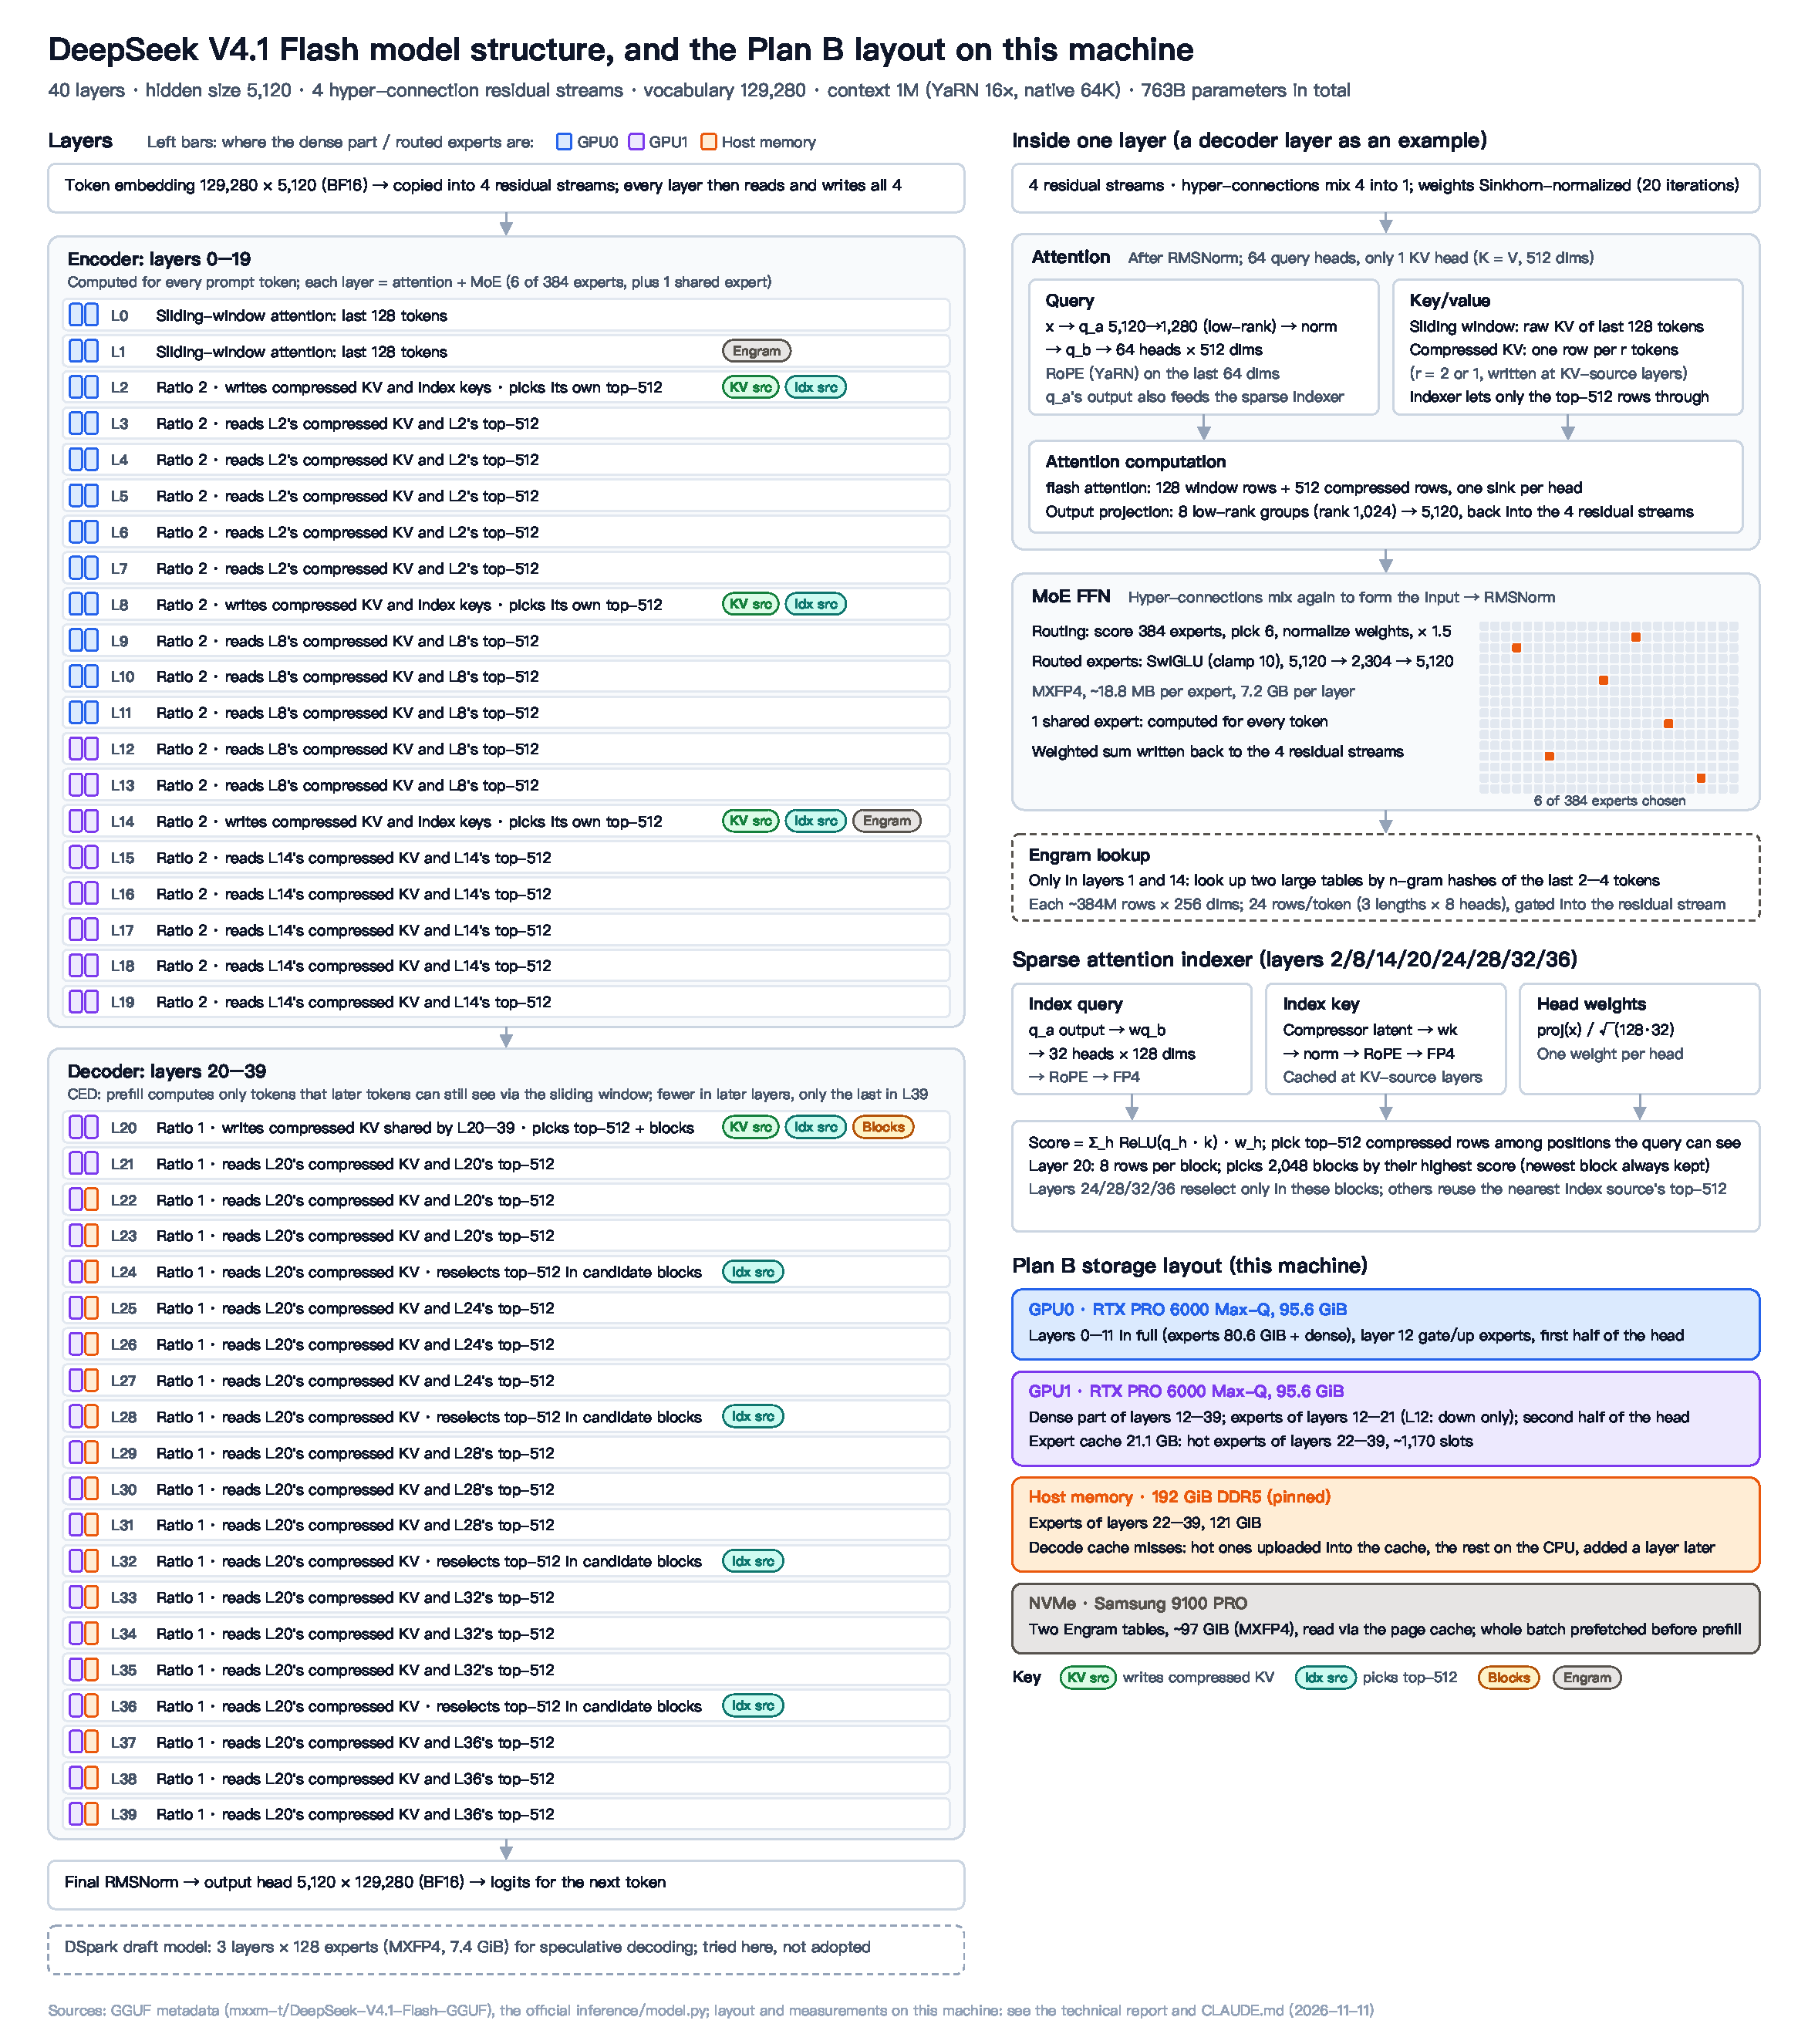
\includegraphics[width=18cm]{figures/architecture-en.pdf}}
  \caption{The layer-by-layer structure of DeepSeek-V4.1-Flash and the Plan B layout on this machine. On the left, each row is one layer, and the color bars show where that layer's dense part and routed experts are placed; on the right are the inside of a single layer, the sparse indexer and the storage layout.}
  \label{fig:arch}
\end{figure}

\subsection{Weight formats and quantization}
\label{sec:formats}

None of the optimizations in this report quantize the model further: they change only which tier the weights are placed in, and which tokens and which rows need not be computed, and every change was cross-checked against the version before it (\S\ref{sec:floors}). The GGUF~\cite{mxllama} we run, however, is itself not quite the same as the official checkpoint. On 11-04 we checked every class of tensors in the GGUF against the official checkpoint, following the rules of the conversion script, by dequantizing samples and comparing them (\code{precision\_audit.py}); Table~\ref{tab:formats} shows the results.

\begin{table}[h]
  \centering
  \small
  \caption{Formats of each class of weights in the GGUF, compared with the official checkpoint (checked class by class against the conversion rules on 11-04; samples were dequantized and compared with the checkpoint's values).}
  \label{tab:formats}
  \begin{tabularx}{\textwidth}{@{}>{\raggedright\arraybackslash}p{4.3cm} >{\raggedright\arraybackslash}p{2.8cm} l r >{\raggedright\arraybackslash}X@{}}
    \toprule
    Weights & Official & GGUF & Size & Precision change \\
    \midrule
    Routed experts & FP4, one scale per 32 values & MXFP4 & 268.9 GiB & None, bit-identical \\
    The 5 attention projections, shared expert, indexer q\_b, Engram wkv & FP8, one scale per 32 × 32 block & Q8\_0 & 6.8 GiB & Relative error 0.55\%, and 0.8\% of nonzero values become 0 \\
    \textbf{Engram tables} & \textbf{FP8, about 189~GiB} & \textbf{MXFP4} & \textbf{97.3 GiB} & \textbf{Relative error 12.0\%, and 9.3\% of nonzero values become 0} \\
    Embedding, output head, router gates, compressors, indexer projections & BF16 & BF16 & 2.6 GiB & None \\
    Sinks, hyper-connection coefficients, router biases, all norms & F32, BF16 & F32 & 0.2 GiB & None \\
    \bottomrule
  \end{tabularx}
\end{table}

The routed experts are bit-identical to the native format. The dense FP8 weights were converted to Q8\_0; both are 8-bit and differ only in how they are scaled, with a relative error of 0.55\%. What actually lost precision is the Engram tables: when the GGUF was made, they were converted from FP8 to MXFP4, which halved their size and also makes them easier to keep in the page cache, at a relative error of 12.0\%, with 9.3\% of the nonzero values becoming 0. This was mxxm-t's choice when converting the original version, and we followed the same rules when we converted the 1017 version (\S\ref{sec:w1017}); NVIDIA made the same conversion in its NVFP4 version and also measured a relative L2 error of about 12\% for the tables, while the scores on benchmarks such as GPQA and SciCode barely changed~\cite{nvfp4}. The cross-checks in this report all compare the same GGUF before and after a change, so we never measured the effect of this step directly; restoring FP8 would require adding an ``E4M3 plus one E8M0 per 32'' type to the fork, and the tables would grow to 189 GiB.

The computation also differs from the official reference implementation in a few places, and most of these differences make it more precise than the official one. Matrix multiplications on both the GPU and the CPU first quantize the activations to int8 in groups of 32 (one F16 scale per group) and then multiply, that is, W4A8; the official implementation uses FP8 activations (one power-of-two scale per 32 values), also 8 bits. On 600 exported router inputs, our activation quantization error was 0.55\%, against 2.65\% for the official method. On Blackwell, the fork's prefill defaults to W4A4 (only 4-bit activations); we changed it back to 8 bits (\S\ref{sec:floors}). The residual stream is F32 (BF16 in the official implementation). The official implementation rounds the sliding-window KV and the attention output to FP8 and the compressed KV to FP4; the fork does not, and stores the KV as F16. The sparse indexer's queries and keys use FP4, which is the official design, and we do the same. The only approximation that changes the computation is expert deferral (\S\ref{sec:defer}).

For comparison, Plan A would further compress the routed experts from about 4.25 bpw to 3.0 bpw, at a KL divergence of 0.0545 relative to the original~\cite{diffbot}; Plan B skips this step, which is exactly why we chose it.

\subsection{The Plan B layout}

Plan B uses a layer split (\code{-sm layer -ts 12/29}): GPU0 holds all of layers 0--11; GPU1 holds the dense parts of layers 12--39 and the experts of layers 12--21; the experts of layers 22--39 (121 GiB) sit in pinned host memory; and the Engram tables stay on NVMe and are read through the page cache. All of the encoder's experts are in VRAM, so as long as the prompt does not go through the decoder layers, prefill barely touches host memory. Table~\ref{tab:place} lists what each tier holds. The GPU1 expert cache added later took 14 GB, and the big-batch split made GPU0's compute buffer about 1.9 GB larger; at a 128K context, the two GPUs had only about 3.6 GB and 1.2 GB left. When the context was extended to 192K, the expert cache dropped to 12 GB (\S\ref{sec:ctx}); on 10-28, after we fixed two places where the compute graph wasted VRAM and chunked the indexer, it grew to 16 GB, and then, after \code{-ot} moved the gate and up expert tensors of layer 12 (about 4.6 GB together) into GPU0's spare VRAM, to 20.5 GB, about 1,140 slots (\S\ref{sec:gpu0cache}); on 11-07, after the output head was split into two halves placed on the two GPUs, it grew to 21.1 GB, about 1,170 slots (\S\ref{sec:headsplit}).

\begin{table}[h]
  \centering
  \small
  \caption{Plan B storage layout (current configuration).}
  \label{tab:place}
  \begin{tabularx}{\textwidth}{@{}l X r@{}}
    \toprule
    Location & Contents & Capacity \\
    \midrule
    GPU0 & Layers 0--11 in full (experts 80.6 GiB + dense parts), the gate and up experts of layer 12, the first half of the output head's rows & 95.6 GiB \\
    GPU1 & Dense parts of layers 12--39, experts of layers 12--21 (only down for layer 12), the second half of the output head's rows, expert cache 21.1 GB & 95.6 GiB \\
    Host memory & Experts of layers 22--39, 121 GiB (CUDA\_Host, pinned) & 192 GB \\
    NVMe & The two Engram tables (MXFP4, about 97 GiB) & 4 TB \\
    \bottomrule
  \end{tabularx}
\end{table}

Figure~\ref{fig:roles} draws the placement and the runtime division of work together. In decode the two GPUs work in series: GPU0 computes only the first 12 layers; GPU1 computes the other 28 and also has to wait for missed experts to be uploaded from host memory, while the CPU computes most of the missed experts at the same time and their results are added back to the residual one layer later (\S\ref{sec:defer}); each GPU computes half of the output head. In prefill, the encoder layers compute all tokens in VRAM, and the decoder layers compute only the tokens near the end of the prompt that are still needed; in layers 22--39, the experts of big batches are uploaded to GPU0 and computed there, as the fork already did, while experts that receive few tokens are computed by the CPU at the same time (\S\ref{sec:bigsplit}) and experts already in the cache are computed directly on GPU1 (\S\ref{sec:bigcache}); for long prompts, the ubatches are pipelined across the two GPUs (\S\ref{sec:overlap}).

\begin{figure}[tp]
  \centering
  \tikzset{
    every node/.style={font=\footnotesize},
    dev/.style={draw, rounded corners=2pt, align=left, inner sep=4pt},
    stage/.style={draw, rounded corners=2pt, align=center, inner sep=3pt, minimum height=1.25cm},
    gpu0/.style={fill=dsblue!10, draw=dsblue},
    gpu1/.style={fill=dsviolet!12, draw=dsviolet},
    host/.style={fill=dsorange!12, draw=dsorange},
    disk/.style={fill=dsgray!25, draw=dsgray!70!black},
    link/.style={{Latex[length=1.6mm]}-{Latex[length=1.6mm]}, line width=0.6pt, dsdark},
    flow/.style={-{Latex[length=1.8mm]}, line width=0.7pt, dsdark},
    lab/.style={font=\scriptsize, fill=white, inner sep=1.2pt, align=center},
  }
  \begin{subfigure}{\textwidth}
    \centering
    \begin{tikzpicture}
      \node[dev, gpu0, text width=6.7cm, anchor=north west] (g0) at (0,0) {%
        \textbf{GPU0}\quad 95.6 GiB, peak use $\approx$94.4 GiB\\[2pt]
        · Layers 0--11 in full + KV (experts 80.6 GiB)\\
        · Gate and up experts of layer 12 ($\approx$4.6 GB)\\
        · First half of the output head rows (631 MiB)\\
        · Prefill: upload staging (layer 22--39 experts)};
      \node[dev, gpu1, text width=6.7cm, anchor=north east] (g1) at (15.5,0) {%
        \textbf{GPU1}\quad 95.6 GiB, peak use $\approx$93.7 GiB\\[2pt]
        · Dense parts of layers 12--39 and their KV\\
        · Layer 12--21 experts (layer 12: down only)\\
        · Second half of the output head rows\\
        · Cache for layers 22--39: 21.1 GB, $\approx$1,170 slots\\
        · Compute buffer $\approx$3 GiB (indexer chunked)};
      \node[dev, host, text width=10.9cm, anchor=north west] (host) at ($(g0.south west |- g1.south)+(0,-1.25)$) {%
        \textbf{Host}\quad Ryzen 9 9950X (16 cores), dual-channel DDR5-6000, 192 GB\\[2pt]
        · Memory: experts of layers 22--39, 121 GiB (pinned); Engram page cache\\
        · CPU, decode: computes $\approx$3/4 of misses, added back a layer later (\code{0025})\\
        · CPU, prefill: computes the experts that receive few tokens (\code{0014})\\
        · CPU, other: Engram row fetch and prefetch (\code{0004}), sampling};
      \node[dev, disk, text width=2.9cm, anchor=north east] (nvme) at ($(g1.south east)+(0,-1.25)$) {%
        \textbf{NVMe}\\[2pt]
        Two Engram tables\\
        MXFP4, 97.3 GiB};
      \draw[link] (g0.south) -- (g0.south |- host.north) node[lab, pos=0.62] {PCIe 5.0 x8\\28.9 GB/s};
      \coordinate (a) at ($(g1.south west)+(1.6,0)$);
      \draw[link] (a) -- (a |- host.north) node[lab, midway] {PCIe 5.0 x8\\28.9 GB/s};
      \draw[link] (g0.north east |- 0,-1.0) -- (g1.north west |- 0,-1.0) node[lab, midway, above=2pt] {P2P\\27.7 GB/s};
      \draw[link] (nvme.west) -- (host.east |- nvme.west) node[lab, midway, above=2pt] {mmap};
    \end{tikzpicture}
    \caption{Placement and links (configuration with a 192K context and a 21.1 GB expert cache, \S\ref{sec:headsplit})}
  \end{subfigure}

  \vspace{0.9em}
  \begin{subfigure}{\textwidth}
    \centering
    \begin{tikzpicture}[node distance=0.55cm]
      \node[stage, gpu0, text width=2.0cm] (d1) {GPU0\\Layers 0--11};
      \node[stage, gpu1, text width=2.0cm, right=of d1] (d2) {GPU1\\Layers 12--21};
      \node[stage, gpu1, text width=3.9cm, right=of d2] (d3) {GPU1\quad Layers 22--39\\Attention, routing,\\cache-hit experts ($\approx$81\%)};
      \node[stage, gpu1, text width=1.55cm, right=of d3] (d4) {Output\\head, half\\per GPU};
      \node[stage, host, text width=1.45cm, right=of d4] (d5) {CPU\\sampling};
      \draw[flow] (d1) -- (d2);
      \draw[flow] (d2) -- (d3);
      \draw[flow] (d3) -- (d4);
      \draw[flow] (d4) -- (d5);
      \node[stage, gpu1, dashed, text width=4.4cm, minimum height=0.9cm] (up) at ($(d3.south)+(-2.5,-1.3)$) {Misses hotter than the victim:\\uploaded over PCIe into the\\cache, computed on GPU1};
      \node[stage, host, text width=3.4cm, minimum height=0.9cm] (cpu) at ($(d3.south)+(2.4,-1.3)$) {The rest: computed\\directly by the CPU,\\deferred a layer (\code{0025})};
      \draw[link] ([xshift=-5mm]d3.south) -- (up.north);
      \draw[link] ([xshift=5mm]d3.south) -- (cpu.north);
      \coordinate (loop) at ($(up.south)+(0,-0.4)$);
      \draw[flow] (d5.south) -- (d5.south |- loop) -| (d1.south) node[lab, pos=0.2] {next token};
    \end{tikzpicture}
    \caption{Decoding one token: the two GPUs in series}
  \end{subfigure}

  \vspace{0.9em}
  \begin{subfigure}{\textwidth}
    \centering
    \begin{tikzpicture}[node distance=0.55cm]
      \node[stage, gpu0, text width=2.2cm] (p1) {GPU0\\Layers 0--11\\all tokens};
      \node[stage, gpu1, text width=2.2cm, right=of p1] (p2) {GPU1\\Layers 12--19\\all tokens};
      \node[stage, gpu1, text width=5.4cm, right=of p2] (p3) {GPU1\quad Layers 20--39\\All KV written; attention and FFN\\only for the tail still needed (CED)\\Cached experts run from slots (\code{0023})};
      \draw[flow] (p1) -- (p2);
      \draw[flow] (p2) -- (p3);
      \node[stage, gpu0, text width=3.7cm, minimum height=0.9cm] (pu) at ($(p3.south)+(-2.0,-1.35)$) {Rest (many tokens):\\uploaded from memory\\and computed on GPU0};
      \node[stage, host, text width=3.3cm, minimum height=0.9cm] (pc) at ($(p3.south)+(2.4,-1.35)$) {Rest (few tokens):\\computed by the CPU\\in compact batches};
      \draw[link] ([xshift=-5mm]p3.south) -- (pu.north);
      \draw[link] ([xshift=5mm]p3.south) -- (pc.north);
      \node[font=\scriptsize, anchor=north west] at ($(pu.south west)+(0,-0.15)$) {Layers 22--39, batches over 32 tokens: three paths at once (\code{0014}, \code{0023})};
      \node[stage, disk, text width=3.7cm, minimum height=0.9cm] (eng) at ($(p1.south)!0.5!(p2.south)+(0,-1.55)$) {Engram (layers 1, 14)\\CPU prefetches NVMe\\rows (n-gram hash, \code{0004})};
      \draw[flow, dashed] (eng.north -| p1.south) -- (p1.south);
      \draw[flow, dashed] (eng.north -| p2.south) -- (p2.south);
    \end{tikzpicture}
    \caption{One prefill call}
  \end{subfigure}
  \caption{How GPU0, GPU1 and the host divide the work in Plan B. Blue is GPU0, violet is GPU1, orange is the CPU and host memory, and gray is NVMe; there is no NVLink between the GPUs, and P2P traffic is forwarded through the CPU. In (b) the two GPUs work in series; with the production settings of 11-08, a token takes about 18.4 ms: about 6.5 ms for layers 0--21, about 10 ms for layers 22--38, about 1.5 ms for layer 39 and the final steps, and about 0.5 ms between tokens (\S\ref{sec:nowtime}). In (c) the encoder layers compute all tokens and the decoder layers only a subset at the end (\S\ref{sec:ced}); for long prompts, GPU0 computes layers 0--11 of the next ubatch while GPU1 computes the later layers of the current one (\S\ref{sec:overlap}).}
  \label{fig:roles}
\end{figure}

% ---------------------------------------------------------------- 3
\section{Evaluation methods}

\subsection{Numerical floors}
\label{sec:floors}

We cross-check with llama.cpp's KL divergence: we first save a set of baseline logits, then compare the logits after a change against them. With early builds, rerunning the same configuration gave identical results (KLD 0); after later patches, the KLD between reruns averaged about 0, with a maximum of about 6e-5 and 100\% top-1 agreement. The important finding is that the numerical floor comes in two tiers (Table~\ref{tab:floors}):

\begin{itemize}
  \item When a change lands only in the decoder layers (layers 20--39), KLD is about 0.0005. An example is computing the experts of layers 22--39 on the GPU instead of the CPU.
  \item When a change passes through the encoder layers (layers 0--19), 0.005--0.01 is normal. For example, computing only the experts of layer 5 on the CPU gives 0.0064; switching kernels, turning off a fusion or changing the ubatch size is of the same order.
\end{itemize}

The reason lies in CED: the encoder's output determines the global KV shared by all positions, so rounding differences there spread to every later position, while differences in the decoder layers affect only the current token. To judge whether a change is correct, one must first establish which tier it falls into.

The same method caught a precision problem at the very start: on Blackwell, mx-llama.cpp defaults to W4A4 for MXFP4 prefill (activations quantized to 4 bits), whereas the official reference implementation is W4A8. As a result, the KLD of the prefill path against the decode path was as high as 0.044, with 91\% top-1 agreement; with 8-bit activations it fell to 0.012 and 95\%, on par with the numerical floor, and prefill was only about 5\% slower.

\begin{table}[h]
  \centering
  \small
  \caption{Numerical floors and the W4A4 problem (2026-10-21).}
  \label{tab:floors}
  \begin{tabular}{@{}l l r@{}}
    \toprule
    Comparison & Scope of the change & KLD \\
    \midrule
    Rerun of the same configuration & --- & 0 (later at most 6e-5) \\
    Experts of layers 22--39 from CPU to GPU & Decoder layers only & 0.0005 \\
    Experts of layer 5 from GPU to CPU & Through encoder layers & 0.0064 \\
    Prefill W4A4 vs.\ the decode path & All layers & 0.044 \\
    Prefill W4A8 vs.\ the decode path & All layers & 0.012 \\
    \bottomrule
  \end{tabular}
\end{table}

\subsection{Cross-checks against the official implementation}

KLD only tells how much the final output changed, not which step caused it. For the parts with complex implementations, we wrote independent reference implementations (oracles) and cross-checked layer by layer: \code{llama-abyss-dump} exports chosen tensors from the fork's compute graph, and PyTorch recomputes them from the same inputs following the official \code{inference/model.py}. The attention of decode steps was also recomputed in float64, to measure the kernels' rounding error on its own. The detailed results are in \S\ref{sec:indexer} and \S\ref{sec:gather}.

\subsection{Profiling}
\label{sec:profiling}

Every performance problem is profiled before we change anything. We capture a stretch of prefill or decode with nsys, total the kernel, copy and idle time per device, and then average per token (\code{tools/eval/nsys\_breakdown.py}, \code{nsys\_decode.py}). Multi-turn agent workloads are measured with a script that imitates Codex: the first turn carries a 48K-token document and two tools, each later turn sends back about 1,500 tokens of tool results or a follow-up question, and cache reuse and prefill time are recorded turn by turn (\code{agent-turns.sh}). For VRAM, \code{GGML\_ALLOC\_TRACE=1} (\code{0019}) records the tensors of every allocation and release in the compute graph, and we list which tensors are present at the compute buffer's peak (\code{alloc-trace.sh}, \code{alloc\_peak.py}).

Profiling CUDA graphs has a trap. nsys has two tracing modes: node-level tracing shows every kernel inside a graph, but it inflates graph launches about 3 times (on 11-06 we measured \code{cudaGraphLaunch} at 2.47 ms per token in total, against only 0.84 ms with whole-graph tracing). Decode profiles before 11-07 all used node-level tracing, so the part with many graph launches (layers 0--21, one or two graphs per layer) came out too large; the gain of tensor parallelism over layers 0--21 was estimated from those profiles and overestimated by more than a factor of two. We now use whole-graph tracing to look at graph launches and the idle time of the two GPUs, and node-level tracing only to look at kernels. To see where the host waits, we use \code{ABYSS\_SYNC\_TRACE} (\code{0044}) in the scheduler and llama-context: it prints every host wait longer than a given number of milliseconds, with the source line, which GPU and which input it waited for; both of the serializing waits in prefill were found with it.

\subsection{PPL on the decode path}
\label{sec:forcedppl}

llama.cpp's perplexity tool processes the whole text in batches, which takes the prefill path; it cannot see changes that take effect only in single-token decode, such as expert deferral. We added forced decoding to \code{llama-abyss-dump} (\code{ABYSS\_DUMP\_FORCE}): after the prompt, instead of sampling, it feeds the next token of a reference text one at a time and records the negative log-likelihood the model assigns to it, so every token goes through the single-token decode path. The two configurations are compared token by token on the same text as paired samples, which gives the PPL difference and its standard error (\code{defer-ppl.sh}, \code{nll\_compare.py}, about 3,100 tokens of corpus text and C++ code). The error of a paired comparison is far smaller than the difference between two independent PPL measurements: expert deferral is +0.06\% ± 0.14\%, and using one expert fewer per token is +1.6\% ± 0.35\%.

\subsection{Fixed seeds and a cold page cache}
\label{sec:seeds}

In the session benchmarks, the temperature-1.0 turns generate different text on every run, so the expert cache hit rates of the two configurations can differ by 2 percentage points, worth about 1\% of decode speed, which is as large as the gain of many changes. Since 11-06, the session benchmarks fix the sampling seed (\code{decode\_modes.py --seed}): when the logits of the two configurations are bit-identical, the whole session is exactly the same and the cache counters match one for one, so any difference comes from the change itself. The other disturbance is the page cache: when the same session runs for the second configuration, the first one has already read the Engram rows into memory, so disk reads cost less than they should; we therefore drop the model files from the page cache before each configuration (\code{DROP\_CACHE=1}).

\subsection{Standard measurements}
\label{sec:stdbench}

For comparison with other systems, we also ran llama-bench and AIPerf (\code{std-bench.sh}, production settings, 16 GB expert cache, Table~\ref{tab:stdbench}). Both measure differently from the rest of this report. Each llama-bench pp test is a single call, so what it mainly measures is the fixed cost of reading the experts of layers 22--39 from memory once per call (about 3 s for 2,048 tokens), and it does not show CED's speedup on long prompts; it uses random tokens, and the cache hit rate in tg is 68--73\%. AIPerf runs at concurrency 1 with a coding corpus and 1,024 output tokens per request: its time to first token (TTFT) is the prefill of a new prompt, and its time per token is close to that of an append-only multi-turn session. The prompts AIPerf generates all begin the same way, so unless the prompt cache is turned off, 12--33\% of the tokens come straight from the cache and the TTFT comes out too low (24.3 s at 96K tokens); the requests therefore need \code{cache\_prompt: false}. AIPerf's \code{--cache-bust} supports only the chat endpoint.

\begin{table}[h]
  \centering
  \small
  \caption{Speed measured with standard tools (2026-10-28, production settings, 16 GB expert cache). llama-bench reads the expert cache size from an environment variable through \code{0021}; AIPerf is version 0.13, at concurrency 1.}
  \label{tab:stdbench}
  \begin{tabular}{@{}l l r@{}}
    \toprule
    Tool & Test & Result \\
    \midrule
    llama-bench & pp512 (depth 0 / 32K / 98K) & about 250 \tps{} \\
     & pp2048 (same depths) & 686 / 678 / 631 \tps{} \\
     & tg128 (same depths) & 32.5 / 33.0 / 34.3 \tps{} \\
    AIPerf & TTFT p50 (input 1K / 8K / 32K / 96K) & 2.70 / 5.53 / 13.25 / 37.1 s \\
     & TTFT p99 (same inputs) & 2.79 / 5.76 / 15.4 / 41.8 s \\
     & Time per token (1,024 output tokens) & 29.4--30.8 ms \\
    \bottomrule
  \end{tabular}
\end{table}

% ---------------------------------------------------------------- 4
\section{Decode}
\label{sec:decode}

Plan B's original decode speed was 16.5 \tps{} (empty context) and about 14.6 \tps{} at a 40K context. The bottleneck was the CPU: for each token, the last 18 decoder layers have to read 108 experts, about 2.0 GB, while memory bandwidth was only 44 GB/s.

\subsection{GPU expert cache}

mx-llama.cpp has a built-in experimental expert cache: it sets aside a group of slots (a bank) on GPU1 and keeps one ``expert id $\to$ slot id'' map per layer; experts that hit are computed directly on the GPU, and misses are uploaded synchronously, with LRU eviction. We gave it 14 GB (about 780 slots, 11\% of the experts in layers 22--39). Expert locality in real text is strong, and the LRU hit rate was about 75\%; decode at a 48K context rose from 14.1 to 25.2 \tps{}, short contexts reached about 29--30 \tps{}, and the KLD was 0.0005.

With the cache on, we profiled decode at a 48K context under PCIe Gen5 (Figure~\ref{fig:decode}): 40.1 ms per token, of which GPU1 uploading missed experts took 17.4 ms (about 26.5 experts, 474 MiB), GPU1 kernels 13.3 ms, GPU0 kernels 4.8 ms and both GPUs idle 4.5 ms, with the parts running mostly in series. Uploads were the largest part.

\begin{figure}[t]
  \centering
  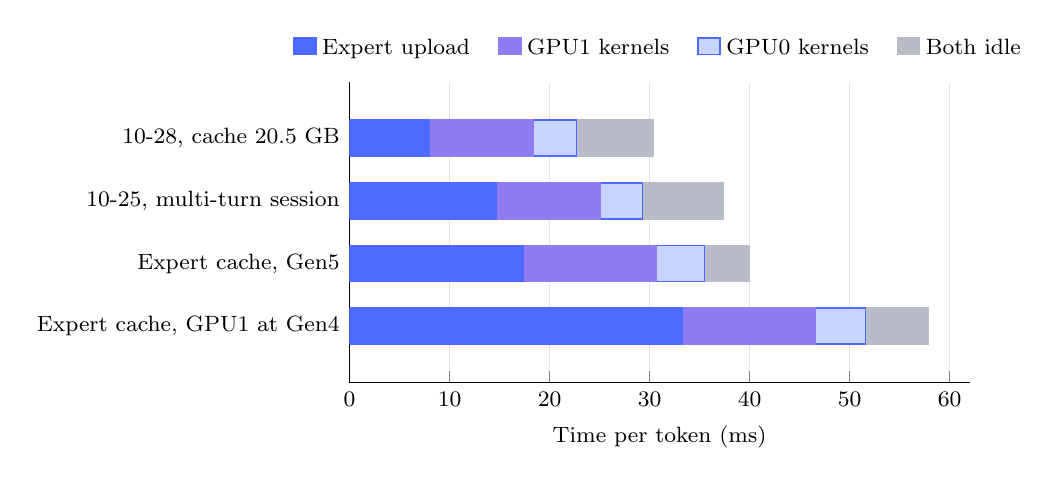
\begin{tikzpicture}
    \begin{axis}[abyss,
      xbar stacked, bar width=13pt,
      width=0.78\textwidth, height=5.4cm,
      xmin=0, xmax=62,
      xlabel={Time per token (ms)},
      ytick={1,2,3,4},
      yticklabels={{10-28, cache 20.5 GB}, {10-25, multi-turn session}, {Expert cache, Gen5}, {Expert cache, GPU1 at Gen4}},
      y dir=reverse,
      ymajorgrids=false, xmajorgrids,
      legend columns=4, legend style={at={(0.5,1.04)},anchor=south,/tikz/every even column/.append style={column sep=8pt}},
      enlarge y limits=0.3]
      \addplot[fill=dsblue,draw=dsblue] coordinates {(8.0,1) (14.7,2) (17.4,3) (33.3,4)};
      \addplot[fill=dsviolet,draw=dsviolet] coordinates {(10.4,1) (10.4,2) (13.3,3) (13.3,4)};
      \addplot[fill=dslight,draw=dsblue] coordinates {(4.3,1) (4.2,2) (4.8,3) (5.0,4)};
      \addplot[fill=dsgray,draw=dsgray] coordinates {(7.7,1) (8.1,2) (4.5,3) (6.3,4)};
      \legend{Expert upload, GPU1 kernels, GPU0 kernels, Both idle}
    \end{axis}
  \end{tikzpicture}
  \caption{Decode time per token (nsys). The last three rows are at a 48K context with memory at 3600 MT/s: the bottom row is from a boot after which GPU1's link trained only to Gen4, making uploads take twice as long (\S\ref{sec:incidents}); the third row is with only the expert cache on; the second row is with all optimizations, in an append-only multi-turn session, at 37.5 ms per token (\S\ref{sec:realdecode}). The first row is the production settings on 10-28 (96K context, memory at 5200 MT/s, 20.5 GB expert cache), at 30.4 ms per token (\S\ref{sec:remaining}).}
  \label{fig:decode}
\end{figure}

\subsection{Decode attention gathers only the top-k rows}
\label{sec:gather}

The profile also showed that about 3 ms of GPU1 kernel time went to \code{concat\_cont}, and that it grew with the context: for every layer and every token, the sliding window and the whole compressed KV were concatenated into one tensor (about 40 µs each time at a 48K context), and flash attention then picked rows by the top-512 mask. For a single query this is wasteful: the query only ever sees 512 compressed rows. We changed it to first take these 512 rows and their mask with \code{get\_rows}, concatenate them with the sliding window, pad to a multiple of 256, and run ordinary flash attention.

Decode at a 48K context rose from 27.7 to 30.6 \tps{}, and at a 128K context from 23.9 to 30.9 \tps{} (both measured on a second generation from the same prompt, \S\ref{sec:realdecode}); decode speed basically no longer drops as the context gets longer. The top-20 KL of temperature-0 generation on the server was about 0.003, above the decoder-layer tier of the numerical floor. We confirmed the cause with a float64 cross-check. Given the same input, both paths see the same set of 640 rows, and both differ from float64 by about 5e-4 (F16 rounding); the difference at layer 20 comes from the layers before it, where rounding differences of about 5e-4 in layers 2--19 are amplified as the MoE chooses between experts with close scores. This is exactly the mechanism behind the encoder-layer tier.

\subsection{Miss split with heat-based admission}

The original design handed all misses to the CPU and swapped experts in only according to a static heat table. Profiling showed that this does not work: LRU's high hit rate relies on swapping in every miss, and without that the hit rate falls to the level of the static heat table (about 47 misses per token), where CPU computation is even slower than uploading; and if the CPU computes an expert and the same expert is then uploaded, it is read from memory twice.

We switched to heat-based admission. A CPU op plans each layer: hits read the cache as usual; among the misses, a fixed fraction is chosen by decayed heat (multiplied by 0.99 per layer per step) and uploaded asynchronously into LRU slots right away; the CPU computes the rest from the original experts in host memory, while the GPU side reads the all-zero slot at the end of the bank, and the two sides are added after the down projection. In the compute graph the CPU branch is expanded before the GPU branch, and the planning op issues the uploads at the start of the CPU split, so the DMA is in flight while the CPU computes the remaining misses, and each expert is read from memory only once.

Table~\ref{tab:admit} shows a sweep of the admission ratio. Uploading only half did not lower the hit rate: only experts picked by heat enter the cache, so rarely used experts do not flush it. We settled on 0.5 (on 10-28, after the expert cache grew to 20.5 GB, a new sweep changed it to 0.3, \S\ref{sec:gpu0cache}): 36.1 \tps{} at a 48K context and 36.2 \tps{} at a 128K context, with a KL of about 2e-4, below the decoder-layer tier. Like the speeds in the table, these two numbers were measured on a second generation from the same prompt and are inflated; real sessions are covered in the next subsection.

\begin{table}[h]
  \centering
  \small
  \caption{Sweep of the admission ratio for misses (48K context, top-k gathering on, 256 tokens generated after reusing the prompt cache, that is, a second, word-for-word identical generation from the same prompt).}
  \label{tab:admit}
  \begin{tabular}{@{}l r r r@{}}
    \toprule
    Admission ratio & Decode (\tps) & Hit rate & Top-20 KL vs.\ uploading all \\
    \midrule
    Upload all (original cache) & 30.6 & 75.5\% & --- \\
    1.0 (new path) & 30.2 & 75.5\% & 0 (bit-identical) \\
    0.5 & 36.1 & 75.9\% & 2.7e-4 \\
    0.4 & 35.7 & 75.1\% & 2.2e-4 \\
    0.3 & 36.4 & 74.5\% & 1.7e-4 \\
    0.2 & 36.0 & 73.1\% & 2.2e-4 \\
    0 (all to the CPU) & 16.1 & 0\% & 1.8e-4 \\
    \bottomrule
  \end{tabular}
\end{table}

\subsection{Decode speed in real sessions}
\label{sec:realdecode}

In real Codex sessions (context about 100K tokens), decode reached only 30--31 \tps{}, clearly below the 36 in Table~\ref{tab:admit}. The difference came from the measurement method: the speeds in the table come from a second generation from the same prompt, which at temperature 0 is word for word identical to the first, so the experts the first one used are still in the LRU cache and the hit rate is inflated; in the same script the first generation reached only 32--35 \tps{}. Codex's own speed test got 47--49 \tps{} at short contexts, also by running the same generation repeatedly.

We switched to measuring with an append-only session (\code{decode\_modes.sh}): the first turn holds documents and tool definitions, and each later turn appends the previous turn's answer and a new question and generates 256 tokens, rotating through greedy or default sampling, streaming or not. Decode was 27--31 \tps{} at a 96K context and 27--29 \tps{} at a 48K context, with no difference among the four modes, matching the real Codex sessions. So decode is affected by neither streaming nor sampling, and it does not slow down as the context grows from 48K to 96K.

\begin{table}[h]
  \centering
  \small
  \caption{Time per token in an append-only multi-turn session (nsys, memory at 3600 MT/s).}
  \label{tab:realdecode}
  \begin{tabular}{@{}l r r@{}}
    \toprule
    Part & 96K context & 48K context \\
    \midrule
    GPU1 uploading missed experts (about 20, 360 MiB) & 14.5 ms & 14.7 ms \\
    GPU1 kernels & 10.5 ms & 10.4 ms \\
    GPU0 kernels & 4.2 ms & 4.2 ms \\
    Both GPUs idle & 7.9 ms & 8.1 ms \\
    Total (under nsys) & 37.1 ms & 37.5 ms \\
    \bottomrule
  \end{tabular}
\end{table}

Table~\ref{tab:realdecode} shows the profile. The kernels that depend on context length (attention, indexer scoring, top-k, row gathering and concatenation) add up to only about 2 ms at a 96K context, and top-k is already a radix select. The timeline of one decoder layer is as follows. GPU1 first computes the merge of the previous layer's experts, this layer's attention and the routing (127 kernels, about 0.47 ms); after the routing result and this layer's input are copied back to the host, one missed expert is uploaded (3 × 6.3 MB, about 0.70 ms) while the CPU computes another (about 0.79 ms); then the CPU result is copied back and the next segment of the compute graph is launched (about 0.09 ms). The upload and the CPU computation together read about 37.6 MB from memory in about 0.8 ms, which is already at the limit of memory bandwidth, and the only GPU work that could be moved into the upload window is this layer's hit experts, under 0.1 ms per layer. So the remaining decode time is mostly the serial handling of misses in each layer, and running the upload in parallel with the hit experts' computation would save at most 2--3 ms per token.

After the memory went up to 5200 MT/s (\S\ref{sec:ddr}), Codex measured once more, with a different short prompt each time: generating 128 or 256 tokens, the median of 9 runs was 40.3 \tps{} (36.8--44.8). Codex's own sessions in the same period (context about 104K) ran at 32.4 \tps{}, consistent with the 31--33 in Table~\ref{tab:ddr5200}. Short contexts are faster partly because the attention-related overhead is smaller (about 2 ms/token at a 96K context) and partly because different generated content gives a different expert cache hit rate; beyond 48K, decode hardly slows down with the context any more.

After Hermes was connected, half of the requests in long sessions (60K--90K context, code and tool output) saw decode drop to 14--26 \tps{}. To find out why, we added decode stats (\code{0016}): every 100 decoded tokens, one line goes to the log with the time per token, the expert cache hit rate, the number of experts per token that hit, were uploaded or were computed on the CPU, and the number of disk page faults. In the slow windows the hit rate, uploads and page faults were the same as usual, and we also ruled out other processes taking the CPU, clock throttling, the PCIe link generation and grammar-constrained sampling; the only correlation was with fewer busy CPU cores, that is, OpenMP threads going to sleep between layers and being woken up again. Setting \code{GOMP\_SPINCOUNT=100000000} makes the threads spin a while longer before sleeping; the average dropped from 43.8 to 35--36 ms/token, and the share of windows over 50 ms fell from 29\% to 7--19\%. The remaining slow windows did not reappear after the shutdown on 10-27, after which GPU1 failed once at boot (\S\ref{sec:incidents}) and the machine was rebooted: the 547 windows after that had a median of 31.1 ms, the slowest 10\% were at 32.8 ms, and none exceeded 50 ms. We have no direct evidence on whether they were related to GPU1's state at the time.

\subsection{Freeing VRAM for the expert cache}
\label{sec:gpu0cache}

Decode speed depends almost entirely on the expert cache hit rate. A fit to several measurements gives a fixed cost of about 15.9 ms per token plus about 0.45 ms for each missed expert (each token makes 108 picks in total across layers 22--39); by this relation, decode without the cache would be about 15.5 \tps{}, which matches the earliest measurement. With a 192K context the cache had only 12 GB (\S\ref{sec:ctx}); on 10-28 we recovered VRAM from three places (Table~\ref{tab:cachegrow}).

\textbf{Two kinds of waste in the compute graph} (\code{0019}). We added \code{GGML\_ALLOC\_TRACE} to ggml's allocator, which records the allocation and release of every tensor each time a compute graph is allocated. The all-zero tensors that \code{0014} adds to each layer were leaves of the compute graph and were all allocated before the graph started (18 × 240 MiB on GPU0); once they were created only when needed, GPU0's usage after loading fell from 94,279 to 91,694 MiB. Under CED, layers with no query rows still computed queries whose results nobody read but which kept holding VRAM (17 × 256 MiB on GPU1); removing them also made prefill 3--5\% faster (96K tokens from 42.6 to 41.2 s), with the output unchanged.

\textbf{Chunking the indexer by query} (\code{0020}). The bulk of GPU1's compute buffer is the sparse indexer's score table and attention mask during prefill, whose size is proportional to ``ubatch × context''. Following DeepInfer, we made scoring and attention handle only one chunk of queries at a time; with 256 queries per chunk the compute buffer dropped from 6.9 GB to 3.2 GB, long prefills became 4--8\% slower, and the KLD against no chunking was 0.0079, within the encoder-layer tier of the floor; the decode compute graph is identical to the one without chunking. The first version of chunking actually used more VRAM: it built a separate mask view for each layer and each chunk, the scheduler copied every view to the GPU, and all inputs of one split were allocated when the split started; usage came down only after each compute graph shared one set of views. We swept chunk sizes of 256, 512 and 1024: GPU1 peaked at 95,880 / 95,906 / 96,684 MiB, and the 96K-token prompt took 44.0 / 42.8 / 42.0 s; 1024 left only about 1.2 GB of headroom, so production uses 512.

\textbf{GPU0's free VRAM}. The cache can only live on the GPU that holds the layers using it: layers 22--39 are all on GPU1, so the roughly 6 GB free on GPU0 was of no use. With \code{-ot} we placed layer 12's gate and up expert tensors (about 2.3 GB each) on GPU0 and gave the space freed on GPU1 to the cache. Layer 12 therefore crosses between the GPUs two more times on each pass, and prefill is 1--2\% slower; moving only the down tensor, with an 18 GB cache, made decode only 2.9\% faster.

\begin{table}[h]
  \centering
  \small
  \caption{Growing the expert cache step by step (2026-10-28, 96K context, append-only multi-turn session, 12 turns per setting). Each row compares before and after one change within the same test run, so the numbers in adjacent rows do not connect.}
  \label{tab:cachegrow}
  \begin{tabular}{@{}l r r r@{}}
    \toprule
    Change & Slots & Decode (\tps) & Hit rate \\
    \midrule
    Indexer chunking, cache 12 $\to$ 16 GB & 670 $\to$ 890 & 31.95 $\to$ 35.42 & 68.4\% $\to$ 74.7\% \\
    Layer 12 gate, up on GPU0, 16 $\to$ 20.5 GB & 890 $\to$ 1,140 & 35.54 $\to$ 38.06 & 74.0\% $\to$ 79.0\% \\
    Admission ratio 0.5 $\to$ 0.3 & 1,140 & 37.75 $\to$ 38.64 & 77.3\% $\to$ 77.2\% \\
    \bottomrule
  \end{tabular}
\end{table}

After the two steps that enlarged the cache, the hit rate rose from 68\% to 79\% and decode became about 19\% faster, in line with the fit's prediction (38.3 \tps{} at 20.5 GB). VRAM was nearly full: GPU0 peaked at 96,386 MiB and GPU1 at about 95,900 MiB, leaving about 1.5 and 2.0 GiB. The output for the 96K-token prompt was identical token for token in all three cache configurations; at 193K tokens the top-20 KL was about 4e-4, because with different cache sizes, different experts are handed to the CPU.

With the larger cache we swept the admission ratio for misses again (\code{admit-sweep.sh}): at 0.1 / 0.2 / 0.3 / 0.5, decode was 36.44 / 37.83 / 38.64 / 37.75 \tps{}, with hit rates of 72.8 / 75.5 / 77.2 / 77.3\%. When the ratio is too low, the cache cannot keep up with newly used experts; at 0.3 the hit rate is already the same as at 0.5, while about 5 fewer experts are uploaded per token. The sweep at 5200 MT/s (\S\ref{sec:ddr}) also found 0.3 slightly better, so production switched to 0.3. After it went live (the evening of 10-28, 53 requests from Hermes and Codex, contexts from 46K to 149K), the 660 decode-stats windows averaged 27.2 ms per token (36.8 \tps{}), the slowest 10\% were at 29 ms, none exceeded 50 ms, and the hit rate was about 79\%, consistent with the speed tests.

\subsection{The 10-28 profile}
\label{sec:remaining}

After the cache grew to 20.5 GB (with the admission ratio still at 0.5), we profiled decode at a 96K context again with the production settings (\code{profile-prod.sh}, first row of Figure~\ref{fig:decode}). Under nsys each token took 30.4 ms: GPU0 compute 4.3 ms, GPU1 uploading missed experts 8.0 ms (about 11.5 experts, 207 MiB, 28.6 GB/s), GPU1 compute 10.4 ms and both GPUs idle 7.7 ms; the four parts were fully serial, and GPU1's uploads did not overlap with its compute. There were 229 calls to \code{cudaStreamSynchronize} per token. \code{nsys\_layer.py} classifies the time when both GPUs are idle by the events before and after it: about 2.2 ms was CUDA graph launches (about 25 per token, about 90 µs each), and about 3.8 ms was the GPUs sitting idle in layers without uploads while the CPU computed experts. In the timeline of one layer, the upload blocks this layer's expert computation, and the next layer in turn waits for this layer's result; only this layer's hit experts can run alongside the upload, so overlapping uploads with computation would save an estimated 1--2 ms per token at most.

We also tried a few cheap switches (\code{quick-knobs.sh}, \code{threads-sweep.sh}, 96K context, 12 turns per setting). Turning off CUDA graphs dropped decode from 38.99 to 36.77 \tps{} ($-$5.7\%); turning on ggml's graph optimization gave 39.20 \tps{}, within the margin of error; we use neither. With 12 / 16 / 24 / 32 CPU threads decode was 38.54 / 37.96 / 37.87 / 36.89 \tps{}, differences within the noise (the hit rate itself fluctuates by about 2 percentage points), so we kept 16: in layers without uploads the GPU is waiting for the CPU to read experts, about 18 MB each, and 16 threads already nearly saturate memory bandwidth. Moving one missed expert from upload to CPU computation saves only about 0.12 ms (an upload takes about 0.66 ms, and the CPU computation is also on the critical path), so moving all uploads to the background would, we estimate, make decode only another 5--10\% faster.

\subsection{Expert prediction and prefetch}
\label{sec:predict}

How much room the cache hit rate still has, and whether misses can be uploaded ahead of time, both depend on which experts each layer actually picks during real decoding. On 11-02 we added temperature sampling to \code{llama-abyss-dump}, decoded a coding task in thinking mode with the production settings, at temperature 1.0 for 4,000 tokens, and at every step dumped the router inputs and selected experts of layers 18--39 (\code{expert-trace.sh}; production was down for less than 4 minutes). Recomputing the routing offline with sqrt-softplus plus bias agreed with the dumped top-6 98--100\% of the time, so this trace can be used for offline simulation (\code{expert\_predict.py}).

\textbf{Cross-layer prediction.} Applying layer $T$'s router gate to layer $T-k$'s router input predicts layer $T$'s experts: with $k=1$, predicting 6 / 8 / 12 / 16 experts covers 75\% / 83\% / 90\% / 93\% of the actual experts; with $k=2$ this falls to 66 / 74 / 82 / 86\%, and with $k=3$ it is 60 / 67 / 76 / 80\%. The previous token's 6 experts in the same layer cover only 33\%, so locality between tokens is far weaker than between layers.

\textbf{Cache policy.} With 1,140 slots, the production policy (admitting only 30\% of misses, chosen by heat, with LRU eviction) had an 80.8\% hit rate, which matches the actual value during the dump (78--81\%); the theoretical optimum that is allowed to leave misses out of the cache (Belady) is 91.2\%, which leaves considerable room. Policy improvements are covered in \S\ref{sec:gate}.

\textbf{Prefetch.} On top of the production policy, uploading the experts missing from the cache ahead of time, according to the prediction from layer $T-1$, cut misses per token in simulation from 20.9 to about 15 when predicting 3. The implementation (\code{0024}, \code{ABYSS\_MOE\_PREFETCH}) applies the next layer's router gate to this layer's router input in layers 22--38 to pick the top $K$ (built the same way as the routing, so CUDA fuses it into one kernel as well); experts not in the cache displace the least recently used slots and are uploaded ahead of time on a second CUDA stream on GPU1, and the next layer's planning makes the main stream wait on its event. The prediction itself was accurate: 88--94\% of the uploaded experts were read, the hit rate rose from 78\% to 82--85\%, misses per token fell by 4--8, and the 32 tokens after the 96K-token prompt were the same as without prefetch. But none of the three ways of issuing the prefetch made decode faster (Table~\ref{tab:prefetch}).

\begin{table}[h]
  \centering
  \small
  \caption{Three ways of issuing expert prefetch (\code{0024}, 96K context, append-only session, 12 turns per setting). Each row is four settings in the same test run, the first without prefetch; each row has a different baseline.}
  \label{tab:prefetch}
  \begin{tabular}{@{}l l l@{}}
    \toprule
    When the prefetch is issued & Predicted/layer (upload cap) & Decode (\tps) \\
    \midrule
    In planning, alongside CPU experts & 0 / 2 / 3 / 4 & 36.27 / 35.74 / 34.25 / 31.88 \\
    After this layer's CPU experts & 0 / 2 / 3 / 3 (2) & 37.71 / 34.44 / 33.46 / 33.83 \\
    After GPU1's layer is submitted & 0 / 2 (1) / 3 (1) / 3 (2) & 38.59 / 38.47 / 38.57 / 38.45 \\
    \bottomrule
  \end{tabular}
\end{table}

nsys showed why (\code{prefetch-profile.sh}, \code{nsys\_streams.py}). Host-to-GPU copies are not split into separate queues; they line up in submission order. With the second way, a 36 MiB prefetch sat in front of the 0.1 MiB small copies that the next segment of computation needs (slot ids and the CPU's results), GPU1 waited idle for 1.28 ms, and the overlap between prefetch and computation was 0\%. The third way added a launch callback to the scheduler and issued the prefetch only after GPU1's computation for this layer had been submitted, which raised the overlap to 43\%; but in layers 22--39 GPU1 computes only about 0.32 ms per layer, while uploading one expert takes 0.67 ms, so the rest of the upload fell into the time the CPU spends computing experts: both-GPUs-idle time dropped from 10.9 to 8.1 ms, but GPU1's busy time rose from 15.2 to 17.8 ms, and the two cancel out.

All three ways fit the same relation: the time per token is about 16 ms of GPU compute plus the expert bytes read from memory divided by about 54 GB/s. The CPU computing experts and uploads to the GPU read the same memory; prefetch only takes a different route, the total bytes do not shrink, and only the part that lands within GPU compute time is saved. Looking one layer ahead hides at most about half, and looking further ahead lowers the accuracy another notch. By this relation, rather than uploading ahead of time, it is better to let the experts the CPU computes run at the same time as the GPU's computation, which is the expert deferral of the next subsection. Prefetch did not go into production.
\subsection{Expert deferral}
\label{sec:defer}

KTransformers~\cite{ktrans} merges the experts handed to the CPU into the residual one layer later, so the GPU does not wait for them. In DeepSeek V4.1 the residual consists of 4 hyper-connection copies: each sublayer first mixes them into one input (hc\_pre) and, after computing, writes the result back with coefficients (hc\_post). We followed this idea in \code{0025} (\code{ABYSS\_MOE\_DEFER=1}): in single-token decode, the experts that layers 22--38 hand to the CPU are not merged into that layer's FFN output; instead, their weighted sum $D_l$ is added into the residual with this layer's FFN post coefficients, before the hc\_post of the next layer's attention (residual $+\,\mathrm{post}_l \otimes D_l$). The residual itself is exact; the only approximation is that the next layer's attention (including its hyper-connection coefficients) does not see this part. Layer 39 has no later layer to defer to, so its CPU experts are still computed synchronously.

The order of the compute graph changes accordingly: GPU1 first computes this layer's experts that hit in the cache and the next layer's attention, while the CPU computes the misses at the same time; the planning operator also copies the FFN input to the host along the way, so the CPU no longer has to wait for the GPU. The scheduler also gained a switch: small inputs (up to 1 MiB) that a GPU split receives from a CPU split go through a pinned staging buffer and are copied asynchronously on the GPU's stream, and a CPU split that directly follows a GPU split and has no inputs no longer synchronizes either, so the host can compute experts while it submits the later computation to the GPU.

With the same build, switch off and on (\code{defer.sh}): an append-only session at 96K context went from 36.59 to 40.63 \tps{} (25.7 to 22.5 ms per token, +11\%), and corpus snippets at short context (about 2K tokens) went from 37.4 to 45.5 \tps{} (+21\%). Numerically, the 32 tokens after a 96K-token prompt were all identical, with a mean top-20 KL of 1.0e-3; on 8 corpus passages of 128 tokens each, the identical prefixes were 16--128 tokens long, with a mean KL of 1.45e-3 and a median of 2.2e-4, and where the outputs diverged, the wording was equivalent in meaning. KL only shows how much the distribution changed. To see whether the approximation hurts quality, we also measured the PPL of the decode path (\S\ref{sec:forcedppl}): over 3,179 tokens of corpus text and C++ code it went from 3.1934 to 3.1955, +0.06\% ± 0.14\%, within the error; for comparison, using one fewer expert per token gives +1.6\% ± 0.35\% (\S\ref{sec:notadopted}). Prefill is not affected.

Once it went live, however, production did not get faster (27--33 ms/token). The reason was that production had the expert heat stats on: they read the routing results through the scheduler's per-node callback, and that path synchronizes the GPU unconditionally after every split, so the host also waited for the split that the GPU runs first to finish, and deferral lost its overlap. None of the test scripts turned the stats on, so the tests did not catch this. After we changed it so that splits from which the callback reads nothing no longer synchronize, a retest with the stats on went from 35.38 to 39.31 \tps{} (+11\%). In production, 109 decode windows from 12 requests (77K--97K context) averaged 24.3 ms/token (41.1 \tps{}), against 27.2 ms before it went live.

\subsection{Expert stats no longer split the graph}
\label{sec:stats}

After deferral we went through the profile kernel by kernel (\code{kernel\_bw.py}, \code{nsys\_kernels.py}). The quantized matrix multiply \code{mul\_mat\_vec\_q} reached 71\% and 73\% of peak bandwidth (1,792 GB/s) on the two GPUs, and the BF16 output head took 811 µs per call at 91\%, so there was little room left. One caveat when reading kernel times: with PDL (programmatic dependent launch) on, a kernel launches early and waits inside for the previous kernel, so the duration of a single kernel in nsys is inflated; its own time has to be taken as ``this kernel's end minus the previous kernel's end''.

The largest item was not in a kernel. The expert heat stats made the fused top-k routing kernel (3 µs) fall back to argsort (14.3 µs, without PDL) plus a string of unfused small kernels, adding 0.76 ms of GPU time per token; the stats' per-node callback also split the compute graph at each layer's selection result, adding one synchronization and one CUDA graph launch per layer (from 25.7 to 82.3 launches per token, each about 42 µs of host time). \code{0026} adds a callback parameter to \code{llama\_context\_params}: when it is set, an output is added for each layer's result after expert selection; when each ubatch finishes, these outputs are copied asynchronously into pinned host memory, just like the logits, and handed to the callback when the logits are read; the per-node callback is no longer installed. With the production settings and deferral on, the 96K session went from 39.11 to 42.17 \tps{} (decode stats 23.6 down to 21.7 ms), against 42.37 with the stats off; greedy generation on short prompts was 13\% faster. With the new stats, the output was identical token for token to the output with the stats off.

Along the way we found that the old stats were wrong for layers 22--39: the callback matched by name prefix, so the reshape and cont that the cache planning and the big-batch split apply to the selection result were counted too. Prefill was counted twice and each decode step once extra, and the one-dimensional view of a big batch was even counted as decode, with 6 times as many picks as the whole batch. For layers 0--21 the old and new stats agreed layer by layer. So layers 22--39 of the stats file have been unreliable ever since the expert cache was turned on, and we started a new file when this went live.

\subsection{Small overheads on the GPU}
\label{sec:kernels}

Once the stats were fixed, the small kernels outside the matrix multiplies and the CUDA graph launches stood out in the GPU time. We made four changes in turn, all to single-token decode only. Except for the first, which passes through the encoder layers and whose KL is within the floor of that tier, the other three give results bit-identical to those before the change.

\textbf{Split-K for the hyper-connection mixing coefficients} (\code{0027}, \code{ABYSS\_HC\_KSPLIT=1}). Each sublayer first applies an unweighted rms\_norm to the flattened residual (4 × 5,120) and then multiplies it by the 24-row mixing-coefficient matrix; the two steps take about 12.3 µs and run 80 times per token. This equals $\mathrm{rsqrt}(\overline{x^2}+\epsilon)\,(Wx)$, so the CUDA backend recognizes the pair and replaces it with two kernels: the first computes, per block, the dot products over a range of columns and the sum of squares over that range; the second adds these up in a fixed order and multiplies by the scale, so the result does not depend on scheduling. The two steps now take 3.3 µs in total. Together with the stats fix, GPU0 kernel time went from 4.48 to 4.00 ms/token and GPU1 from 11.02 to 9.96 ms, and the session went from 41.97 to 43.86 \tps{} (+4.5\%). The mean KL over the 8 corpus passages was 3.8e-3, in the same encoder-layer tier as \code{0008}.

\textbf{Small-kernel fusion} (\code{0032}). Single-token decode runs about 2,900 kernels per token, and those outside the matrix multiplies take about 3.9 ms. The hyper-connection chain (the post gate after the mixing coefficients, Sinkhorn, the pre gate of the next sublayer, merging the copies, and rms\_norm) is folded into the split-K reduction kernel and one merge kernel; the KV assembly in attention (gathering the top-k rows, converting them to F16 and appending them after the window; gathering the mask rows, repeating, converting and concatenating; 7 kernels, about 0.53 ms) becomes a single kernel. This removes about 290 kernels and 0.57 ms of GPU kernel time per token, and the decode stats went from 19.8 to 19.3 ms. The first version of the KV assembly fusion gave wrong results: in the original graph, once the mask's columns have been taken, nothing uses the mask input any more, so the allocator gave its memory to the concatenated mask. Running the kernels separately is fine, but the fused kernel reads and writes at the same time and goes wrong. The unit test allocates each tensor separately, so it could not catch this. The fusion now checks, one by one, the tensors the kernel reads against the address ranges of the two outputs, and does not fuse if any of them overlap.

\textbf{The tail of the matrix multiplies} (\code{0036}, \code{ABYSS\_MMVQ\_TAIL=1}). We added performance cases with this model's decode shapes to the unit tests (all 32 experts selected, so the data read exceeds the L2). The MXFP4 expert down projection (5,120 × 2,304) reached only 62\% of peak: with 128 threads per thread block and K split into quantization blocks, each row has 72 blocks; the first round covers 64 of them and the second round only 8. Matrix multiplies whose last round of the K loop leaves many threads idle now compute several rows per thread block at once (the summation order within each row is unchanged); in the microbenchmark the down projection went from 179.5 to 143.9 µs. With only 6 experts computed and gate and up fused, the grid is too small and several rows per block is slower instead, so that case is excluded. In the production profile, the matrix-vector multiplies took about 0.24 ms less per token.

\textbf{Launching CUDA graphs in two parts} (\code{0038}, \code{ABYSS\_GRAPH\_CHUNK=128}). All earlier profiles used node-level tracing, which inflates graph launches about threefold. With whole-graph tracing there were 46 launches per token, 0.84 ms on the host, and each launch of the two largest graphs (layers 0--11 on GPU0 and layers 13--21 on GPU1, each with over 400 kernels) took 150--170 µs, all on the critical path. A graph with more than 512 nodes is now cut in two after its 128th node, and the second part is submitted while the first runs. The idle wait at the start of the two large graphs went from 280 and 295 µs to 137 and 180 µs, and the session went from 51.49 to 52.04 \tps{} (about +1\%). A first version that cut at 128, 256, 512 nodes and so on was slower: each cut leaves the GPU idle for 5--12 µs, and the small per-layer graphs were cut too, which cancelled the gain.

\subsection{Engram disk reads during decode}
\label{sec:engramdecode}

Engram sits in layers 1 and 14. In single-token decode, each of these layers fetches 24 rows from the mmapped table; the CPU row fetch forms a split of its own in the graph, and a row that is not in the page cache means waiting for the NVMe. In the profile, GPU0 sat idle for 962 µs on average (median 640) before the Engram projection of layer 1, and GPU1 for 278 µs before layer 14, about 1.2 ms per token in total, all on the critical path; the prefetch of \code{0004} only covers batches of 64 or more tokens. We measured several ways of reading on the two tables (\code{engram\_reads.c}, with about 34 of the rows not in the page cache each time): touching the rows one by one took 2,896 µs, about 86 µs per cold row, which is what the original row fetch does; issuing \code{MADV\_WILLNEED} for these 48 rows first and then touching them took 184 µs; touching them in parallel from 16 threads took 387 µs. \code{0028} issues \code{MADV\_WILLNEED} right after the row numbers are computed. The GPU idle wait dropped to 0.49 ms/token in total, and the output was identical token for token.

Of the remaining 0.49 ms, 84\% came from a few tokens that each stalled for about 9.2 ms. That is the NVMe drive's automatic power saving (APST): after 100 ms idle, the 9100 PRO enters a state that takes about 9.5 ms to exit; when the page cache is warm, several tokens in a row do not read the disk, and the next cold read runs into it. With APST turned off for this drive (by writing \code{pm\_qos\_latency\_tolerance\_us} at runtime, and through a udev rule at boot), the first read took about 600 µs no matter how long the drive had been idle. Measured more finely: after up to 5 ms idle the first read took 73--97 µs, after 10 ms about 280 µs, and after 15 ms or more 560--650 µs. A token takes about 19 ms and cold rows are read only once per token, at its start, so the read hits the slowest tier every time. \code{0039} has a background thread read a random 4 KiB of the table file with direct I/O every 4 ms during single-token decode, so the drive never goes to sleep (\code{ABYSS\_ENGRAM\_KEEPALIVE\_MS=4}). In four alternating runs of 19 turns each, the session went from 50.71 to 51.19 \tps{} (+1\%), and in offcputime the main thread's wait for disk reads went from 14.1 ms to 0.3 ms per second; the cost is about 1 MB of reads per second during decode. Production has many cold rows: the two tables total 104 GB and the page cache holds only about 52 GB; bpftrace counted an average of 24.5 pages read from disk per token, and 67\% of tokens read at least one page.

\subsection{The cache admission gate and eviction}
\label{sec:gate}

On the routing trace from \S\ref{sec:predict}, we simulated several combinations of admission and eviction, this time also counting uploads per token (\code{cache\_policy.py}, Table~\ref{tab:policy}). Changing only the eviction from LRU to ``lowest decayed heat'' raised the hit rate from 80.5\% to 81.4\%. Adding an admission gate on top, ``admit only if hotter than the one it would evict'', while still admitting at most 30\% of the misses, kept the hit rate the same at a decay factor of 0.99 and cut uploads per token from 6.3 to 4.7. A decay of 0.999 is too sticky (77.6\%), and the admission gate with LRU eviction is worse.

\begin{table}[h]
  \centering
  \small
  \caption{Cache policies simulated on the 11-02 routing trace (1,140 slots shared by layers 22--39).}
  \label{tab:policy}
  \begin{tabular}{@{}l r r r@{}}
    \toprule
    Policy & Hit rate & Misses/token & Uploads/token \\
    \midrule
    Production: admit 30\% of misses by heat, LRU eviction & 80.5\% & 21.0 & 6.3 \\
    Evict lowest decayed heat instead & 81.4\% & 20.0 & 6.0 \\
    Plus admission gate, decay 0.995 & 80.5\% & 21.0 & 2.9 \\
    \textbf{Plus admission gate, decay 0.99 (deployed)} & \textbf{81.4\%} & \textbf{20.0} & \textbf{4.7} \\
    Admission gate with no ratio cap, decay 0.99 & 82.6\% & 18.7 & 7.7 \\
    \bottomrule
  \end{tabular}
\end{table}

Implementation (\code{0030}): on eviction, it scans the whole group of slots for the one with the lowest decayed heat (empty slots first; slots read by the current planning step or just admitted are not evicted); when a miss fails the admission gate, admission stops and the rest go to the CPU. In single-token decode, the experts computed by the CPU get slot number $-1$, and the matrix multiply writes zeros for the whole block on a negative id instead of reading the all-zero slot. Four configurations with the production settings, a 12-turn session each: the old production ran at 45.32 \tps{} (decode stats 20.5 ms/token), and all three changes on with decay 0.99 ran at 46.75 \tps{} (+3.2\%, hit rate 79.2\%, 5.2 uploads and 17.3 CPU-computed experts per token). Decay 0.995 was a little faster still (46.95), but it defers more experts and its heat reaches further back, so production uses 0.99. Part of the saved uploads turned into extra experts computed by the CPU, so the gain was smaller than the roughly 2 ms the simulation estimated. The mean KL against the old production was 6e-4, in the same tier as expert deferral: some of the experts handed to the CPU and deferred changed.

\subsection{Sampling and the time between tokens}
\label{sec:sampling}

Decode speed measured per request is always lower than the decode stats suggest: the stats time only \code{llama\_decode}, not the GPU's finishing work after it returns, sampling, or the server's own processing. \code{0033} adds timing to every step of the server. The server's own processing (main loop, queues, assembling the batch, streaming) takes only about 0.04 ms per token and does not grow however long the reply gets; outside \code{llama\_decode} there is the 0.90 ms wait for the GPU to finish (0.81 ms for the BF16 output head plus copying the logits back) and sampling (about 0.24 ms at temperature 1.0).

We changed sampling in two steps. At temperature 1.0 and top\_p 1.0, only \code{dist} does any work in the sampler chain: it calls \code{expf} on each of the 129,280 logits one by one, accumulates in double, and then divides one by one. \code{0029} switches to a polynomial exp that can be auto-vectorized, sums in blocks, and finds the block holding the target before searching within it; in a microbenchmark that loads only the vocabulary, this went from 0.411 to 0.117 ms/token, and over 2,000 draws with a fixed seed the chosen tokens were all identical. For \code{0035} we noticed that with the production parameters every sampler in the chain except \code{dist} does nothing, yet the original path still builds a 129,280-entry candidate array every token. When the chain holds only such samplers plus \code{dist} (or greedy), it now samples directly from the logits: at temperature 1.0 this went from 0.232 to 0.069 ms per token, and fixed-seed requests were identical token for token.

\subsection{Output head split across the two GPUs}
\label{sec:headsplit}

Most of the 0.9 ms spent waiting for the GPU to finish goes to the BF16 output head (129,280 × 5,120, 1.32 GB): all of it sits on GPU1, while GPU0 is idle at that point. \code{0034} (\code{ABYSS\_HEAD\_SPLIT=0.5}) copies the first half of the rows to GPU0 at load time; for a single output, each GPU computes one half, and the halves are joined on GPU0 and copied back to the host. Each row is still the same dot product, so the logits are bit-identical. We ran into three problems along the way. The second half used a view created at graph-build time; the view had no buffer yet, so the scheduler did not recognize it as a weight on GPU1 and assigned that half's matrix multiply to GPU0 as well, copying 631 MiB per token. Using \code{-ot} disables pipeline parallelism, so the scheduler has no events, and when switching GPUs the host had to synchronize with the previous GPU, which made the two halves run serially. And ``wait until the destination GPU is done with this memory'' before a cross-GPU copy was another host synchronization. For this, the scheduler gained a path in which a GPU that follows another GPU does not synchronize but waits on an event on the GPU instead. As a result, the wait for the GPU went from 0.91 to 0.53 ms per token, and the session from 47.83 to 48.54 \tps{}. The cost is 631 MiB more on GPU0, which leaves only about 0.7 GB free after loading, so the desktop can no longer use GPU0.

After this, GPU1 computes only the second half, and its copy of the first half is used only when a batch has multiple outputs. So \code{0040} no longer loads the output head as a whole: each half is read from the file onto its own GPU (\code{ABYSS\_HEAD\_SPLIT\_ONLY=1}), and the number of outputs per batch is limited to the number of sequences (which is 1 in the server anyway). GPU1 uses 630 MiB less, which went to the expert cache, raising it from 20.5 GB to 21.1 GB, about 1,170 slots: the session went from 51.77 to 52.04 \tps{} and the hit rate from 80.6\% to 81.3\%. The MTP block and the DSpark draft model read the whole output head, so they cannot be enabled at the same time.

\subsection{Where the time goes now}
\label{sec:nowtime}

With the production configuration of 11-08, the decode stats show about 18.4 ms/token, and per request about 50 \tps{}. The time per token is: layers 0--21 about 6.5 ms, GPU only, with the two GPUs taking turns (inferred from the measurements of the 11-09 tensor parallelism prototype; the 8--9 ms that nsys measured under node-level tracing is too high); layers 22--38 about 10 ms; layer 39 and the finish about 1.5 ms; between tokens about 0.5 ms.

The time of layers 22--38 is set by host memory bandwidth and the serial segments in each layer. In the 11-04 profile, each of these 17 layers forms one window, from one planning step to the next: per token there were 12 windows without an upload at 0.58 ms each and 4.8 with one upload at 1.13 ms each. The 0.66 ms upload is queued on the same stream as GPU1's computation; in windows with an upload, the CPU and PCIe read host memory together, about 61 GB/s combined (CPU about 32, upload about 29), which is the limit of the memory bandwidth, and the CPU's own experts take as long as the upload anyway. In the 11-07 profile, layers without an upload took 0.547 ms each: GPU1 kernels 0.306 ms, the host's own computation (planning plus the CPU experts) 0.334 ms, and the host waiting for the GPU 0.133 ms. GPU1 starts computing the hit experts about 70 µs after the routing finishes, and the CPU's results arrive just as it is done. Of the roughly 3.8 ms with both GPUs idle, about 1.9 ms is the 100--130 µs per layer by which the CPU's part takes longer than GPU1's in layers 22--38, about 0.3 ms is the CPU experts of layer 39, which cannot be deferred, and planning and launches take about 45 µs per layer.

Of the roughly 0.5 ms between tokens, 0.41 ms is on the main thread. The parts we could identify are sampling at 0.14 ms (the test requests carry \code{ignore\_eos} and take the slow path; in production it is about 0.07 ms), the \code{madvise} for the Engram read-ahead plus the OS kernel's read-ahead at about 55 µs, fetching and dequantizing the rows at about 15 µs, and the rest of input preparation at about 50 µs combined; no single item dominates.

So even if all of the host memory traffic were hidden under GPU computation, each token would still take about 15 ms (about 67 \tps{}); to go faster, we can only reduce the GPU computation (layers 0--21) or the experts read from memory.

\subsection{Tried but not adopted}
\label{sec:notadopted}

\textbf{One fewer expert per token.} Strata~\cite{strata} uses only 5 experts per token in its default ``Faster'' mode on four R9700s. We tried it with \code{--override-kv deepseek41.expert\_used\_count=int:5} (\code{experts5.sh}), with the selected experts' weights normalized as usual. In an append-only session at 48K context, decode went from 32.6 to 36.8 \tps{} (+13\%): the experts dropped are the ones ranked 6th, which are less popular, so misses fell by 26\% and the hit rate rose from 65.8\% to 69.5\%; the small prefill of each turn was also about 10\% faster. But the KLD against 6 experts was 0.032 and the top-1 agreement 91.9\%, and PPL rose from 5.863 to 5.954 (+1.6\% ± 0.35\%): that is 3--6 times the numerical floor and about 60\% of that of 3.0 bpw quantization (KL 0.0545), and it cancels half of the PPL improvement from switching to 1017. Strata measured no difference at 2.25 bpw because its quantization error (KL 0.107) masked it. Production still uses 6.

\textbf{DSpark speculative decoding.} The fork's \code{draft-dspark} supports V4-style draft models, and the 1017 sidecar (\S\ref{sec:w1017}) works with it directly (\code{dspark.sh}). Writing code greedily at 64K context, decode went from 31.1 to 36.2 \tps{} (+16\%), with 4.3--4.5 tokens accepted per verification on average and a draft acceptance rate of 66--70\%. The ceiling on the gain is low: one verification has the main model compute 6 tokens, which use more experts, so the misses multiply; it takes about 120 ms, 3.8 times a single token, so even with all 5 drafts accepted it is only about 1.6 times as fast. There are three more problems. The draft model's weights are 7.6 GB and its compute buffer 2.3 GB, so the expert cache has to shrink to 6 GB to make room, which by itself lowers decode at 48K context from 32.6 to 28.0 \tps{} and cancels the gain. The draft model reads the hidden states of layers 37--39, so CED cannot skip the decoder layers during prefill, and the first-turn prefill of 48K tokens went from 23.4 s to 91.7 s. Long prompts also leave a gap in the draft model's KV positions (after writing up to 33,112, the next batch starts at 48,222), and the request fails with HTTP 500. The greedy output diverges from the non-speculative one at characters 104--315; at the point of divergence the choices are nearly equivalent, and the divergence comes from the numerical differences between batched verification and single-token decode. We did not adopt it for now. When we rechecked on 11-07, the conditions were worse: the VRAM freed since then had all gone to the expert cache (21.1 GB), so enabling it would mean cutting the cache to about 10 GB and also giving up the output head loaded only as two halves (\S\ref{sec:headsplit}); the decode optimizations since then (expert deferral, split-K, small-kernel fusion, gathering only the top-k rows) all apply only to single tokens, so the 6 tokens of a verification cannot use them; and at production's temperature of 1.0 the acceptance rate is also lower than in the greedy runs measured here. The +59--76\% reported externally on 4 GPUs was measured with all experts in VRAM, where a verification costs barely more than a single token.

\textbf{Deferring the uploaded experts too.} After expert deferral, in layers with an upload, this layer's hit experts and the next layer's attention must wait for the upload to finish before they can start (\S\ref{sec:nowtime}). \code{0031} (\code{ABYSS\_MOE\_DEFER\_UPLOAD=1}) stops uploading the first admitted miss of each layer during planning: once the computation for the hits has been submitted, that expert is uploaded on a second stream on GPU1 and then added back into the residual in the next layer together with the CPU experts. Now 40\% of the upload overlapped with kernels, but the session was only about 1\% faster (46.75 to 47.23 \tps{}), and the decode-path PPL changed by +0.12\% ± 0.10\%. The gain was small for two reasons. In layers with an upload, the CPU and PCIe read host memory together, so the bottleneck is memory bandwidth, not the upload being queued ahead of the computation. And the matrix multiply still launches one thread block per row for a $-1$ expert, which exits as soon as it starts; in the first version this cost GPU1 an extra 0.44 ms per token. It did not go into production. Along the way we also tried having the thread blocks loop over the ids and skip $-1$: the output was bit-identical, but with fewer thread blocks the parallelism was lower, and it was slower instead (48.32 down to 48.12 \tps{}).

\textbf{q8\_1 activation cache.} The fork has a built-in cache that quantizes the same input only once, but it evicts first in, first out, which conflicts with the last-in, first-out release order of the CUDA memory pool and triggers an assertion, so production always kept it off. \code{0036} gives it its own legacy pool, which cut the quantization calls in decode from 426 to 322 per token, but an hour after it went live, GPU0's free VRAM had dropped to about 230 MiB and was still falling, so we turned it back off: the legacy pool keeps freed blocks for reuse, and since the number of tokens per layer varies in prefill, the sizes of the cached entries vary with it. \code{0037} limits the dedicated pool to entries of at most 128 KiB, which uses the same VRAM as having the cache off, but the gain is only about 0.3--0.5\%, so it did not go into production.

\textbf{A Q8\_0 output head.} The BF16 output head reads 1.32 GB per token; as Q8\_0 it is 0.70 GB, with a relative weight error of 0.54\% (\code{retype\_tensor.py} copies only the shard that holds this tensor and requantizes it in the copy). The session was 2.1\% faster (about 0.4 ms less per token), with a mean top-20 KL of 5.5e-4 and a decode-path PPL change of $-$0.01\% ± 0.02\%. It is not below 4 bits, but it introduces quantization error into weights that were not quantized before, so we did not adopt it.

\textbf{Three ideas we estimated and dropped.} Temporarily uploading the misses handed to the CPU into spare slots, so that the CPU and PCIe share the memory bandwidth: most layers have only 0--1 CPU experts, and a single expert over PCIe (0.66 ms) is slower than the CPU reading it (0.38 ms), so this would save only 0.23 ms per token (\code{cpu\_dma\_balance.py}). Biasing the cache toward layer 39, which cannot be deferred: with its heat multiplied by 4, the experts layer 39 hands to the CPU per token fell from 1.07 to 0.54, but the other layers got 0.9 more misses, and most of their CPU experts are on the critical path too. Not making the hit experts wait for host planning (keeping an ``expert $\to$ slot'' table on the GPU and computing the hits as soon as the routing is out): the CPU path is the real bottleneck, since it must first read back the routing and finish planning before it can compute the misses, and the next layer waits for its results, so starting the GPU early only makes it wait longer; we estimated a saving of only 0.1--0.2 ms per token, for several days of work.

% ---------------------------------------------------------------- 5
\section{Prefill}
\label{sec:prefill}

The original fork also runs all 40 layers over the prompt: every 2,048-token ubatch has to read the 121 GiB of decoder-layer experts in host memory once. A 48K-token prompt therefore takes 135 s (about 355 \tps{}).

\subsection{CED-aware prefill}
\label{sec:ced}

The official reference implementation also runs all 40 layers over the prompt; CED shows up in how the KV is shared: in the decoder layers, only the sliding window uses each layer's own hidden states. This allows exact pruning: layers 0--19 compute all tokens; layer 39 computes only the last token; layer $L$ (20--38) needs to compute only the last $128 + 127 \times (38-L)$ tokens---with each earlier layer, the sliding window extends the dependency another 127 tokens back. The implementation originally kept 256 extra positions at the end for speculative-decoding rollback; without DSpark, DSV4 cannot roll back partially, so the default was later changed to keep none (\S\ref{sec:tailmerge}). The decoder layers then come to about 24K ``token × layer'' units in total, independent of the prompt length; for a 48K-token prompt, the original fork computes $20 \times 48{,}240 \approx 960$K of them (Figure~\ref{fig:ced}).

\begin{figure}[t]
  \centering
  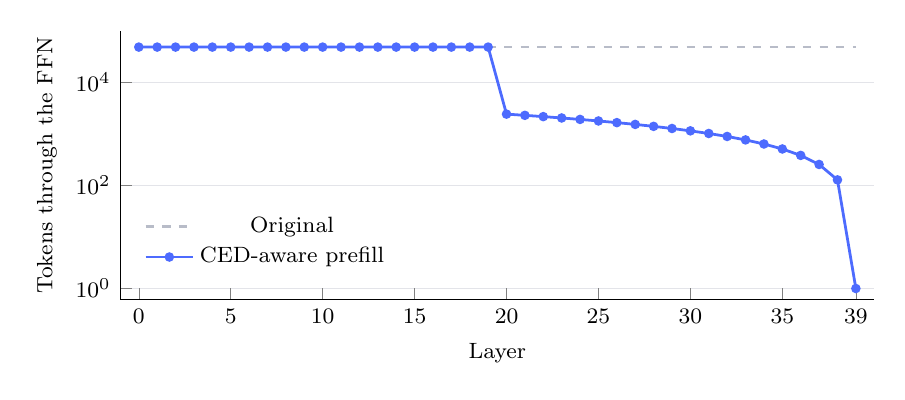
\begin{tikzpicture}
    \begin{axis}[abyss,
      width=0.92\textwidth, height=5.0cm,
      ymode=log, ymin=0.6, ymax=1e5,
      xmin=-1, xmax=40,
      xlabel={Layer}, ylabel={Tokens through the FFN},
      xtick={0,5,10,15,20,25,30,35,39},
      legend style={at={(0.02,0.08)},anchor=south west}]
      \addplot[dsgray, mark=none, line width=1pt, dashed] coordinates {(0,48240) (39,48240)};
      \addplot[dsblue, mark=*, mark size=1.2pt, line width=1pt] coordinates {
        (0,48240) (1,48240) (2,48240) (3,48240) (4,48240) (5,48240) (6,48240) (7,48240) (8,48240) (9,48240)
        (10,48240) (11,48240) (12,48240) (13,48240) (14,48240) (15,48240) (16,48240) (17,48240) (18,48240) (19,48240)
        (20,2414) (21,2287) (22,2160) (23,2033) (24,1906) (25,1779) (26,1652) (27,1525) (28,1398) (29,1271)
        (30,1144) (31,1017) (32,890) (33,763) (34,636) (35,509) (36,382) (37,255) (38,128) (39,1)};
      \legend{Original, CED-aware prefill}
    \end{axis}
  \end{tikzpicture}
  \caption{Number of tokens per layer whose FFN is computed, for a 48K-token prompt (from the planning rule in the implementation; with DSpark off, no margin is kept). The encoder layers compute every token; the decoder layers compute only the tokens that later tokens can still see through the sliding window.}
  \label{fig:ced}
\end{figure}

We implemented it in two steps. The first step (\code{0003}) skips only the FFN: attention is still computed for all tokens, and the KV writes are completely unchanged. The skipped tokens' hidden states are wrong in the layers after that, but they only enter sliding windows that no later token reads. Each \code{llama\_decode} call plans from its own end, so the server uses \code{-b 65536} to put the whole prompt into one call. Prefill of a 48K-token prompt dropped from 135 s to 41.8 s; the cross-check at 8k/16k context gave a KLD of 0.00006 / 0.00004 and a top-1 agreement of 99.8\%.

The second step (\code{0005}) began with a profile: of the 41.8 s at that point, attention in layers 20--39 took 19.9 s. We made these layers still write KV for all tokens, but compute attention only for the CED subset, taking out just its query and mask rows. Prefill dropped to 27.9 s (1,715 \tps{}), with a KLD of 0.00004--0.00007, and the temperature-0 output matched the first step's character for character.

\subsection{Engram prefetch}

The Engram tables are mapped with mmap with a random-access hint, and every page fault synchronously reads one 4 KiB page; 2,048 tokens take about 2.4 s, and the bottleneck is page-fault latency, not SSD bandwidth. Since the row indices depend only on the input tokens, we compute all of them as soon as \code{llama\_decode} receives the whole batch; 8 background threads sort them by address and read them ahead with \code{MADV\_WILLNEED}. With a cold page cache, prefill of a 48K-token prompt dropped from 91.1 s to 54.3 s, and the cold-read overhead from about 39 s to about 2 s; with a warm cache it did not change, and the results were identical to those without prefetch. The cold reads are now mostly hidden behind computation, so further steps such as io\_uring and a per-row cache are on hold.

\subsection{Adding the official sparse indexer}
\label{sec:indexer}

The fork originally did dense attention over V4.1's compressed KV. With at most 512 compressed rows this is equivalent to the official top-512 selection; beyond that it differs: after about 512 tokens in the layers with compression ratio 1, and after about 1,024 tokens in the layers with compression ratio 2. Agent contexts are almost all in this range, so this is first of all a correctness issue.

Following the official \code{inference/model.py}, we added the complete indexer: the KV source layers write FP4 index keys (blocks of 32, scale $2^{\lceil \log_2(\mathrm{amax}/6) \rceil}$), the index source layers compute $\sum_h \mathrm{ReLU}(q_h \cdot k)\, w_h$ and select the top 512, layer 20 picks the candidate blocks, and the other layers reuse the result of the nearest index source; flash attention looks only at the selected positions. Within 512 tokens, the KLD against the dense version is 0; at 8k/16k/32k context, the sparse version's PPL is 0.9\% / 3.1\% / 0.23\% lower than the dense version's (Table~\ref{tab:sparse}). Because attention looks at only 640 rows, prefill of a 48K-token prompt also dropped from 27.9 s to 22.7 s, and a 128K-token prompt took 51.8 s (2,464 \tps{}).

\begin{table}[h]
  \centering
  \small
  \caption{Sparse indexer vs.\ dense attention (perplexity, 4 segments per context length).}
  \label{tab:sparse}
  \begin{tabular}{@{}l r r r r@{}}
    \toprule
    Context & PPL (dense) & PPL (sparse) & Change & KLD, sparse vs.\ dense \\
    \midrule
    8k & 6.023 & 5.972 & $-0.9\%$ & 0.057 \\
    16k & 3.009 & 2.916 & $-3.1\%$ & 0.094 \\
    32k & 1.0027 & 1.0004 & $-0.23\%$ & 0.012 \\
    \bottomrule
  \end{tabular}
\end{table}

To confirm that the implementation matches the official one, we dumped the indexer inputs and outputs of layers 2, 20 and 24, recomputed the top-512 with three kinds of arithmetic and compared the overlap (Table~\ref{tab:oracle}): float32 throughout; the fork's arithmetic (the Q8\_0 matrix multiply quantizes the activations to int8); and the official arithmetic (bf16 activations, quantized to e4m3 for an FP8 GEMM). The fork overlaps with its own arithmetic by more than 99.98\%, which shows that every step is correct: RoPE/YaRN, FP4, the weight scaling, visibility and top-k. The fork is closer to float32 (98.7--99.2\%) than the official algorithm itself is (97.1--98.7\%). More than 99.99\% of the index keys are bit-identical; the ones that differ are all single elements that fall exactly on an FP4 midpoint.

\begin{table}[h]
  \centering
  \small
  \caption{Average overlap of the top-512 sets (4,027-token prompt).}
  \label{tab:oracle}
  \begin{tabular}{@{}l r r r r@{}}
    \toprule
    Layer & Fork vs.\ int8 ref. & Fork vs.\ float32 & Official arith.\ vs.\ float32 & Fork vs.\ official arith. \\
    \midrule
    2 & 99.99\% & 99.16\% & 98.67\% & 98.63\% \\
    20 & 99.98\% & 98.67\% & 97.14\% & 97.11\% \\
    24 & 99.98\% & 98.85\% & 97.40\% & 97.36\% \\
    \bottomrule
  \end{tabular}
\end{table}

\subsection{Big-batch split}
\label{sec:bigsplit}

In a multi-turn session each turn adds relatively few tokens, but as soon as a batch exceeds 32 tokens, nearly all 384 experts of layers 22--39 get used, and the scheduler offloads the expert matrix multiplies of these big batches to GPU0, uploading each layer's experts in full. In the prefill of one 1,610-token turn (7.0 s), GPU0 spent 5.4 s uploading 145 GiB, while the CPU, GPU1's link and the expert cache sat idle. The floor for this part is one read of these experts from memory, about 3 s.

We extended the idea of the miss split to big batches: in each layer, a CPU op counts the tokens of each expert and hands experts to the CPU in order from fewest tokens to most, until the CPU's estimated time catches up with the upload time of the remaining experts; the rest are uploaded to GPU0 as before. For this we added handling of id = $-1$ to CUDA's MMQ (skip it and zero the output), and the upload callback uses the planning op's result on the host directly instead of reading the ids back from the GPU.

The first version's CPU branch processed the whole tensor (all tokens × 6 experts), while the CPU actually computed only about 5\% of the rows; quantization, SwiGLU, zeroing and copying back the 252 MB output ate up all of the gain, and it was slower than no split at all. After switching to compact batches---taking out only the ``token × expert'' pairs handed to the CPU (at most 1,024 rows), gathering those tokens on GPU1, computing one expert per row on the CPU, writing the results back with \code{set\_rows} and adding them to GPU0's result---prefill of a 2,048-token batch dropped from 4.88 s to 4.24 s, with a KLD of 0.00046. In the multi-turn session, the prefill of each later turn dropped from 5.7--7.2 s to 4.6--5.6 s, and the first turn from 30.6 s to 27.9 s (Figure~\ref{fig:agent}).

\begin{figure}[t]
  \centering
  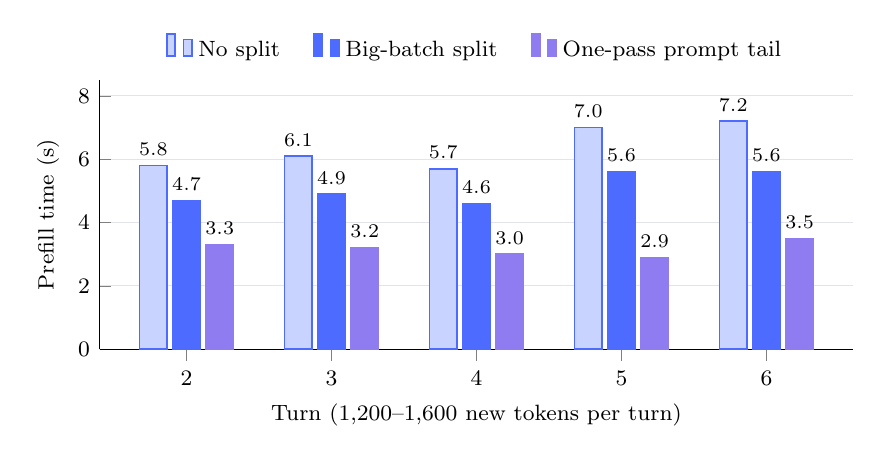
\begin{tikzpicture}
    \begin{axis}[abyss,
      width=0.92\textwidth, height=5.0cm,
      ybar, bar width=10pt, ymin=0, ymax=8.5,
      xlabel={Turn (1,200--1,600 new tokens per turn)}, ylabel={Prefill time (s)},
      xtick={2,3,4,5,6},
      nodes near coords={\pgfmathprintnumber[fixed,fixed zerofill,precision=1]{\pgfplotspointmeta}},
      nodes near coords style={font=\scriptsize},
      legend columns=3, legend style={at={(0.5,1.03)},anchor=south,/tikz/every even column/.append style={column sep=10pt}},
      enlarge x limits=0.15]
      \addplot[fill=dslight,draw=dsblue] coordinates {(2,5.8) (3,6.1) (4,5.7) (5,7.0) (6,7.2)};
      \addplot[fill=dsblue,draw=dsblue] coordinates {(2,4.7) (3,4.9) (4,4.6) (5,5.6) (6,5.6)};
      \addplot[fill=dsviolet,draw=dsviolet] coordinates {(2,3.3) (3,3.2) (4,3.0) (5,2.9) (6,3.5)};
      \legend{No split, Big-batch split, One-pass prompt tail}
    \end{axis}
  \end{tikzpicture}
  \caption{Prefill time per turn in a multi-turn agent session (the first turn is a 48K-token document; each later turn feeds back a tool result or asks a follow-up question; memory at 3600 MT/s). For the one-pass prompt tail, see \S\ref{sec:tailmerge}.}
  \label{fig:agent}
\end{figure}

This step is still about 30 ms/layer above the floor: GPU0's upload staging buffer is reused for the three weights gate, up and down, so every segment boundary needs a synchronization, and the CPU has to wait until the gate batch has been transferred before it can start (on 11-09 we found that this synchronization is the host waiting; see \S\ref{sec:nowait}); CPU compute and DMA also share 44 GB/s of memory bandwidth. The merge steps have to be pinned to GPU0; otherwise GPU1's compute buffer grows by 3.7 GB and does not fit at 128K context. While implementing this we also found and fixed a bug in the fork (\code{0013}): \code{ggml\_backend\_sched\_reserve\_size} resets the scheduler before splitting the compute graph, which clears the backends assigned by hand while the graph is built, so the compute buffers are estimated from the wrong split.

\subsection{One-pass prompt tail}
\label{sec:tailmerge}

CED makes every \code{llama\_decode} call run the decoder layers relative to its own end, so every call longer than 32 tokens has to read nearly all experts of layers 22--39 from memory once. To build checkpoints, the server splits calls at the start of the last user message, at 4 + n\_ubatch before the end, and at 4 before the end. In the production logs, most Codex turns were therefore split into two large calls (for example 1,772 + 866 + 4), which cost 1.5--2 s more than turns of the same length with only one call; and when the tail of one call spans two ubatches, the experts are read twice as well. We made three changes (\code{0015}):

\begin{itemize}
  \item Within the last 2,700 tokens of the prompt, calls are no longer split at the start of a user message or at 4 + n\_ubatch before the end; only the split 4 tokens before the end remains, and the next turn uses it to continue from the assistant prefix. The session's first checkpoint is kept as before; Codex's auxiliary requests rely on it to reuse the system prompt. The cost is that these two kinds of checkpoints are gone: they would only matter when the last user message is rewritten, in which case the server falls back to the previous turn's checkpoint and computes one extra turn.
  \item The remainder of a call goes into the first ubatch, so the last ubatch is a full 2,048 tokens. Previously the remainder came last, the last ubatch often had only a few hundred tokens, and roughly layers 20--32 had to be computed once more in the ubatch before it; now the ubatch before it has only a few tokens left, in layers 20--22.
  \item The margin at the end now defaults to the depth of the rollback ring, \code{n\_rs\_seq}, which is 0 without DSpark. We checked position by position against the planning formula that, with a margin of 0, the sliding-window state that the next token needs is still complete.
\end{itemize}

\begin{table}[h]
  \centering
  \small
  \caption{Effect of the one-pass prompt tail (\code{agent-turns.sh}, memory at 3600 MT/s).}
  \label{tab:tailmerge}
  \begin{tabular}{@{}l r r@{}}
    \toprule
    Configuration & First turn, 48K tokens & Next 5 turns (1,200--1,600 tokens) \\
    \midrule
    Before & 27.9 s & 4.6--5.6 s \\
    No call splits in the tail & 25.3 s & 3.2--3.7 s \\
    + last ubatch aligned to full & 24.4 s & 3.2--3.7 s \\
    + margin of 0 & 24.0 s & 2.9--3.5 s \\
    \bottomrule
  \end{tabular}
\end{table}

We measured new prompts the way external benchmarks do (prompt cache off, median of 3 runs per setting): 2,324 tokens dropped from 5.57 s to 3.69 s, and 4,277 tokens from 8.80 s to 4.34 s. In the cross-check, aligning the last ubatch gave a KLD of 0.0092 and a top-1 agreement of 95.4\% against the version before the change, the same as only changing the ubatch from 2048 to 1024 (0.0090, 96.0\%); a margin of 0 and a margin of 256 generated the same 256 tokens (top-20 KL 4.6e-4). We also built prompts directly from token arrays so that the call length modulo 2,048 was 0, 1, 2, 7--9, 31--33, 127--129, 1000 and 2047, at about 2K, 4K and 20K tokens each; all 42 requests worked correctly.

\subsection{Big batches from the cache}
\label{sec:bigcache}

After the one-pass prompt tail, each turn's prefill still had a large fixed cost: a fit over the 92 prefills in the production logs from the afternoon of 10-28 gave about 1.84 s per prefill plus about 0.98 ms per new token, so even a Hermes turn that added only 505 tokens took 2.2 s. We had assumed that CED makes the decoder layers compute only the last 128 or so tokens of each turn. Using \code{0022} to print, for each big batch, how many experts it used and how many of those were already in the cache (\code{big-coverage.sh}), we measured that when a turn adds 1,100--2,800 tokens, each batch in each of layers 22--38 has about 860--1,140 tokens and uses about 240 experts: under CED, the decoder layers still compute most of the new tokens. By count, only 22\% of these experts were in GPU1's cache, but by number of selections it was 55\%: the cache holds the experts that decode uses often, and they also receive more tokens.

The planning at the time handed about 126 experts per batch to the CPU (13 of them in the cache) and uploaded 116 from memory to GPU0 to be computed there, 40 of which were in fact already in GPU1's cache: the cache can only copy to the GPU it lives on, but big batches were computed on GPU0, so these were uploaded from memory anyway. A profile of one turn (1,609 new tokens, 3.2 s): GPU0 uploading 37 GiB of experts from the host took 1.37 s, GPU0 compute 0.52 s, GPU1 compute 0.61 s (attention 0.22 s, of which the indexer 0.13 s), GPU1 transfers 0.11 s, and both GPUs idle 0.63 s; again it was mostly serial.

\code{0023} makes the planning op record the slots of the experts already in the cache; these experts are computed directly on GPU1 from their slots (gate, up, activation, down, then the weighted sum), and the rest are split between the CPU and uploads to GPU0 as in \code{0014}. In the compute graph, the GPU0 path is issued first, then the GPU1 path, and the CPU computes last; the three run at the same time, and their results are added. We ran the same session once with it off and once with it on (\code{big-cache.sh}, Figure~\ref{fig:bigcache}): turns of the same length were 0.3--0.4 s faster (about 11\%), and over the whole session about 20\% of the big-batch experts were computed from the cache instead; long new prompts were essentially unchanged, because the cache is cold and only 16\% hit. GPU1's VRAM after loading and at peak were both unchanged: the new path's intermediate tensors do not coincide with the peak. For the cross-check, we first greedily decoded 512 tokens from a short prompt to fill the cache identically in both runs, then ran a 96K-token prompt: the 32 output tokens were identical, with a top-20 KL of 1.7e-4.

\begin{figure}[t]
  \centering
  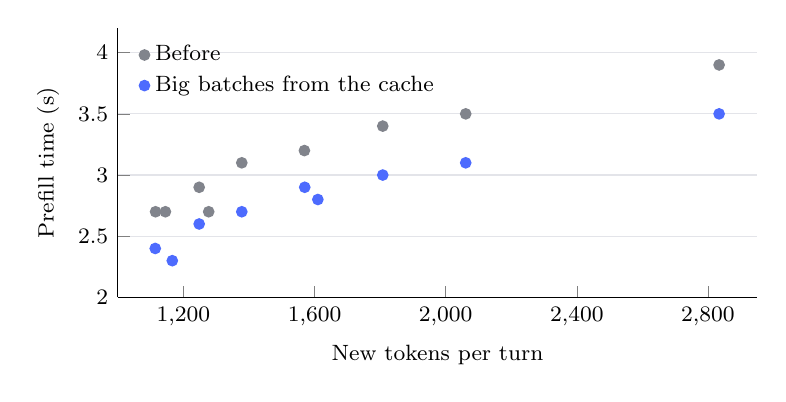
\begin{tikzpicture}
    \begin{axis}[abyss,
      width=0.80\textwidth, height=5.0cm,
      xmin=1000, xmax=2950, ymin=2, ymax=4.2,
      scaled x ticks=false, xtick={1200,1600,2000,2400,2800},
      xlabel={New tokens per turn}, ylabel={Prefill time (s)},
      legend cell align=left, legend style={at={(0.02,0.98)},anchor=north west}]
      \addplot[dsgray!70!black, only marks, mark=*, mark size=1.8pt] coordinates {(1115,2.7) (1145,2.7) (1248,2.9) (1277,2.7) (1378,3.1) (1569,3.2) (1808,3.4) (2061,3.5) (2834,3.9)};
      \addplot[dsblue, only marks, mark=*, mark size=1.8pt] coordinates {(1114,2.4) (1166,2.3) (1248,2.6) (1378,2.7) (1570,2.9) (1610,2.8) (1808,3.0) (2061,3.1) (2834,3.5)};
      \legend{Before, Big batches from the cache}
    \end{axis}
  \end{tikzpicture}
  \caption{Prefill time per turn in a multi-turn agent session (\code{big-cache.sh}; first turn 96K tokens, then 9 turns; memory at 5200 MT/s, expert cache 20.5 GB). The two sessions did not generate exactly the same text, so two of the turns differ in their number of new tokens.}
  \label{fig:bigcache}
\end{figure}

\subsection{Two-GPU pipeline for long prompts}
\label{sec:overlap}

Upstream llama.cpp has an unmerged PR (\#29963) that pipelines several GPUs even when the experts are in host memory; its author measured long prompts 1.5--2 times faster on 3 RTX PRO 4000 cards. We first measured our own case (\code{prefill-pipe.sh}, \code{nsys\_pipe.py}, the second request of a 96K-token prompt): of the 40.6 s, both GPUs were busy at the same time for only 0.21 s; GPU0 was busy for 22.8 s and GPU1 for 15.0 s. Each of the 41 encoder-only ubatches took 755 ms: layers 0--11 on GPU0 took 409 ms, the handoff of layer 12 between the two GPUs 17 ms, the remaining layers on GPU1 295 ms, and both GPUs were waiting for 34 ms (Figure~\ref{fig:overlap}a). If GPU1 computed the later layers of one ubatch while GPU0 computed layers 0--11 of the next, we estimated about 27 s.

The fork has a built-in pipeline (\code{pipeline\_parallel}), but it is turned off when \code{-ot} or the expert cache is used, and it stores an extra copy of every input for each pipeline copy, held for the whole graph: when reserving for a 196K context, a single compressed-attention mask is 384--768 MiB, so GPU0 would need 1.1 GiB more and GPU1 3.3 GiB more, which does not fit. So we kept a single copy and removed only the serialization points. Of the main thread's 40.6 s, 29.3 s were spent in \code{cudaStreamSynchronize}; recorded with \code{ABYSS\_SYNC\_TRACE}, they came mainly from three places: waiting for GPU1 to finish before copying request inputs (masks and so on) to it (13.8 s); stopping both GPUs before re-allocating the compute graph for each ubatch (7.9 s: GPU0's copy of the mask grows with the KV and outgrows the previous allocation); and waiting for the target GPU before copying from the CPU to it (4.6 s). What \code{0044} (\code{ABYSS\_OVERLAP=1}) changes:

\begin{itemize}
  \item When the target GPU still has work queued, large inputs go through a pinned staging buffer and are transferred in order on that GPU's stream, without making the host wait; when the GPU is idle or the input is under 1 MiB, they are still copied directly as before, since otherwise each turn of a multi-turn session would pay an extra memory copy of a few hundred MiB. Each input alternates between two staging buffers on each GPU, each with its own event; a staging buffer that has grown is released only at the next synchronization, because freeing pinned memory synchronizes the whole GPU.
  \item A new graph layout is first only planned, and if no buffer has to grow, the GPUs are not stopped: the next ubatch's writes to a GPU's VRAM are all queued behind the work already on that GPU.
  \item Zero-byte inputs are neither copied nor waited for. Between the two halves of the output head (\S\ref{sec:headsplit}) there is a hidden state with 0 rows; at the end of every ubatch it added a ``wait for GPU1 to finish copying'' to GPU0's stream, and that copy was queued behind all of GPU1's compute for the ubatch, while layers 0--11 of the next ubatch were all queued behind this wait: this was the direct reason the two GPUs kept taking turns. In nsys, the kernels had been submitted 1.5 s ahead, yet GPU0 still sat idle for about 280 ms at the start of every ubatch; we found the cause only by listing the operations on GPU0's stream in submission order.
  \item The expert stats used to synchronize once per ubatch to hand over the selection results; they now alternate between two pinned buffers.
\end{itemize}

In addition, the environment variable \code{CUDA\_SCALE\_LAUNCH\_QUEUES=4x} has to be set: GPU1 has about 1,300 kernels per ubatch, and the host otherwise blocks on CUDA's launch queue while submitting them; with only \code{ABYSS\_OVERLAP} the prompt took 33.4 s, and with this variable as well 29.0 s. Direct access between the two GPUs (\code{GGML\_CUDA\_P2P}) had no effect on prefill.

\begin{figure}[t]
  \centering
  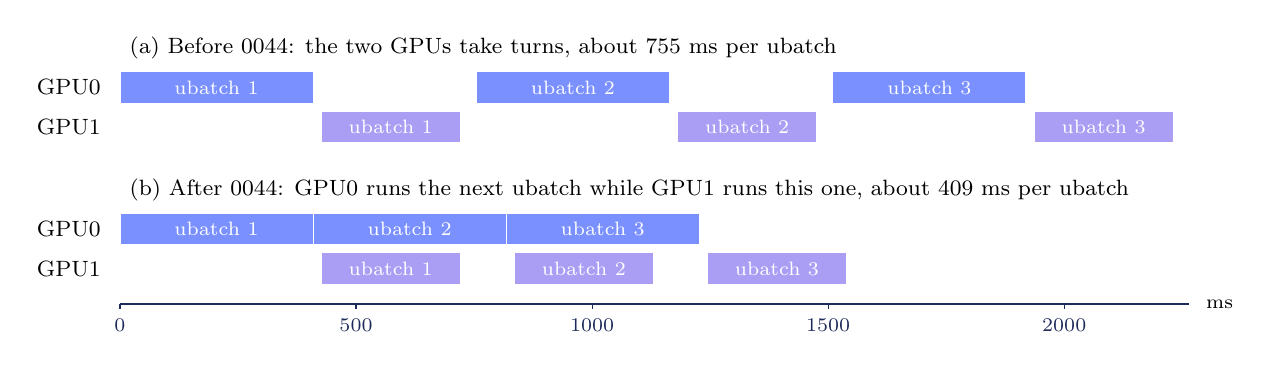
\begin{tikzpicture}[x=0.0060cm, y=1cm]
    \tikzset{
      g0/.style={fill=dsblue!75, draw=white, line width=0.4pt},
      g1/.style={fill=dsviolet!75, draw=white, line width=0.4pt},
      ub/.style={font=\scriptsize, text=white},
      row/.style={font=\footnotesize, anchor=east},
    }
    % (a) before: the two GPUs take turns, about 755 ms a ubatch
    \node[font=\footnotesize, anchor=west] at (0,1.05) {(a) Before 0044: the two GPUs take turns, about 755 ms per ubatch};
    \node[row] at (-20,0.55) {GPU0};
    \node[row] at (-20,0.05) {GPU1};
    \foreach \k in {0,1,2} {
      \pgfmathsetmacro{\a}{755*\k}
      \pgfmathsetmacro{\b}{755*\k+409}
      \pgfmathsetmacro{\c}{755*\k+426}
      \pgfmathsetmacro{\d}{755*\k+721}
      \pgfmathtruncatemacro{\n}{\k+1}
      \draw[g0] (\a,0.35) rectangle (\b,0.75) node[ub, midway] {ubatch \n};
      \draw[g1] (\c,-0.15) rectangle (\d,0.25) node[ub, midway] {ubatch \n};
    }
    % (b) after: GPU0 computes the next ubatch while GPU1 finishes this one
    \node[font=\footnotesize, anchor=west] at (0,-0.75) {(b) After 0044: GPU0 runs the next ubatch while GPU1 runs this one, about 409 ms per ubatch};
    \node[row] at (-20,-1.25) {GPU0};
    \node[row] at (-20,-1.75) {GPU1};
    \foreach \k in {0,1,2} {
      \pgfmathsetmacro{\a}{409*\k}
      \pgfmathsetmacro{\b}{409*\k+409}
      \pgfmathsetmacro{\c}{409*\k+426}
      \pgfmathsetmacro{\d}{409*\k+721}
      \pgfmathtruncatemacro{\n}{\k+1}
      \draw[g0] (\a,-1.45) rectangle (\b,-1.05) node[ub, midway] {ubatch \n};
      \draw[g1] (\c,-1.95) rectangle (\d,-1.55) node[ub, midway] {ubatch \n};
    }
    % time axis
    \draw[dsdark, line width=0.5pt] (0,-2.2) -- (2265,-2.2);
    \foreach \t in {0,500,1000,1500,2000} {
      \draw[dsdark] (\t,-2.2) -- (\t,-2.27) node[below, font=\scriptsize] {\t};
    }
    \node[font=\scriptsize, anchor=west] at (2280,-2.2) {ms};
  \end{tikzpicture}
  \caption{Timeline of the encoder-only ubatches (2,048 tokens) of a long-prompt prefill on the two GPUs, a schematic drawn from the per-segment times in the profile of a 96K-token prompt; the GPU0 row is layers 0--11, and the GPU1 row is layer 12 and later. In (a), GPU0 has to wait at the start of every ubatch for GPU1 to finish the previous one; in (b), both GPUs are busy at the same time, and the time per ubatch is set by layers 0--11 on GPU0 (\S\ref{sec:overlap}).}
  \label{fig:overlap}
\end{figure}

With the same build, the switch off and on, and stats on in both: a 96K-token prompt dropped from 40.9 to 28.7 s ($-$30\%), filling 193K tokens from 83.5 to 58.1 s, and the first agent turn (48K tokens) from 21.2 to 15.1 s; each later turn has only one ubatch, so nothing gets pipelined, and 2.30 vs.\ 2.32 s is the same; session decode was 50.12 vs.\ 50.48 \tps{}. The outputs of the 8 corpus segments, the 96K-token prompt, passkey retrieval at 193K tokens and the 10-turn agent session were all identical token for token, and peak VRAM was only 18 MiB higher. GPU0 is now the bottleneck (Figure~\ref{fig:overlap}b); going faster would mean moving layers, which touches GPU1's expert cache. Having both GPUs compute the early layers together is another route, but in the prototype of Section~\ref{sec:tp} the two GPUs compute the first 20 layers together, so this pipeline no longer applies, and long prompts were actually 8\% slower.

\subsection{Small calls created by checkpoint splitting}
\label{sec:ckptsplit}

Long prompts are split into calls at the start of user messages to build checkpoints, following \code{--checkpoint-min-step 32768} (\S\ref{sec:restart}). A checkpoint is built only after the batch has been assembled, right before \code{llama\_decode} is called, and it stores the state at the start of that call; but when the batch-assembly loop decides where to cut next, it still measures the step from the previous checkpoint. So a call that has just passed the step, and will build a checkpoint at its start, gets cut again at the next user message, leaving a small call of a few hundred tokens that builds no checkpoint, while under CED every call has to read the experts of layers 22--39 once. The first long request after the restart at 23:42 on 11-08 (77K tokens) was split into 33,279, 381, 32,665, 318, 10,627 and 4 tokens, and the two small calls took about 1.7 s each; in the logs since 10-20, 32 requests had 48 such small calls, about 109 s in total.

\code{0045} (\code{ABYSS\_CKPT\_COUNT\_START=1}) makes the loop count the checkpoint at the start of the current call: the next cut measures the step from the start of this call, and the tail merge of \S\ref{sec:tailmerge} also takes effect from that checkpoint on. The same patch also makes each request log one more line saying how many calls its prompt was split into, how many tokens each had and where checkpoints were built; at the default log level, the small calls near the start used to be invisible. We tested with two long multi-message conversations (\code{ckpt\_split.py}): computing 96K tokens in 16 messages of about 6K each from scratch went from 6 calls to 4 (35,425 + 35,183 + 25,483 + 4) and from 36.0 to 30.6 s; a 112K-token agent session with messages of varying length went from 8 calls to 5 and from 42.1 to 36.9 s; recomputing after editing one message about 60\% of the way in, each of the two needed one call fewer and was 2.7 s and 1.5 s faster, respectively. The checkpoint positions did not change. Because the split changed, the ubatch boundaries changed with it: over the 89 tokens of common output prefix, the weighted average top-20 KL was 8.2e-3, within the encoder-layer tier of the numerical floor, and every divergence was between near-tied candidates. The upstream llama.cpp server has the same check.

\subsection{Not making the host wait before big-batch uploads}
\label{sec:nowait}

As \S\ref{sec:bigsplit} noted, the big-batch split was still about 30 ms/layer above the floor, which we had attributed to GPU0's uploads and compute not being pipelined. On 11-09 we measured first (\code{big-pipe.sh}, \code{nsys\_big.py}; turn 6 of an agent session, 1,095 new tokens, prefill 2.1 s): in each of layers 22--39, the experts assigned to GPU0 are uploaded in three segments, gate, up and down, each taking 10--21 ms (29 GB/s), and after each segment GPU0 computes for only 1--2.5 ms; hiding all of that compute inside the uploads would save at most 0.09 s, which is not worth doing. The time actually went to waiting: of the 1.60 s spent in these 17 layers, both GPUs were idle for 0.45 s, and the host waited in synchronization for 0.92 s. \code{ABYSS\_SYNC\_TRACE} showed that the scheduler made the host wait for GPU0 to finish before copying weights from the host (34 times per turn, 620 ms in total): the host was stuck there, the CPU's share of the experts could start only after all three segments had been queued, and once the GPU was done it in turn waited for the CPU.

The copy is queued on GPU0's own stream in any case, after the compute that uses the same VRAM, so stream order alone already makes it safe; the paths that read device data or modify host data (the expert-cache lookup has to read the expert ids) already synchronize on their own. \code{0046} (\code{ABYSS\_WEIGHT\_NOWAIT=1}) removes the wait before host weights that are handed to the copy callback. Comparing the two settings with the page cache dropped: the prefill of the 9 later turns of an agent session dropped on average from 2.33 to 1.96 s ($-$16\%, Figure~\ref{fig:nowait}), the 48K-token first turn from 14.7 to 14.1 s, and a new 96K-token prompt from 27.6 to 26.8 s; decode was unchanged (18.5 ms/token). The outputs for the corpus and the 96K-token prompt were bit-identical, peak VRAM was 16 MiB higher, and that wait went from 36 times and 742 ms per turn to zero. The host waits that remain are for GPU1 to compute the routing before each layer's planning, which is a true dependency.

\begin{figure}[t]
  \centering
  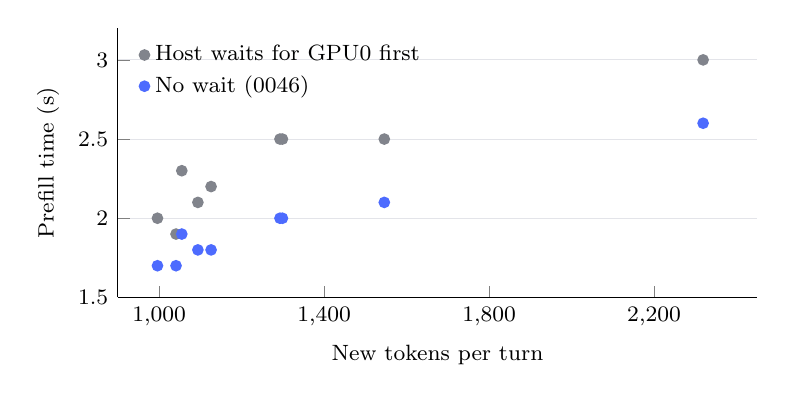
\begin{tikzpicture}
    \begin{axis}[abyss,
      width=0.80\textwidth, height=5.0cm,
      xmin=900, xmax=2450, ymin=1.5, ymax=3.2,
      scaled x ticks=false, xtick={1000,1400,1800,2200},
      xlabel={New tokens per turn}, ylabel={Prefill time (s)},
      legend cell align=left, legend style={at={(0.02,0.98)},anchor=north west}]
      \addplot[dsgray!70!black, only marks, mark=*, mark size=1.8pt] coordinates {(1299,2.5) (1126,2.2) (996,2.0) (1041,1.9) (1094,2.1) (1055,2.3) (1293,2.5) (1546,2.5) (2319,3.0)};
      \addplot[dsblue, only marks, mark=*, mark size=1.8pt] coordinates {(1299,2.0) (1126,1.8) (996,1.7) (1041,1.7) (1094,1.8) (1055,1.9) (1293,2.0) (1546,2.1) (2319,2.6)};
      \legend{Host waits for GPU0 first, No wait (0046)}
    \end{axis}
  \end{tikzpicture}
  \caption{Prefill time of each later turn in an agent session (\code{agent\_turns.py}; first turn 48K tokens, then 9 turns that feed back tool results or ask follow-up questions; memory at 6000 MT/s, expert cache 21.1 GB, page cache dropped before each setting). Every turn had exactly the same input in both settings.}
  \label{fig:nowait}
\end{figure}

% ---------------------------------------------------------------- 6
\section{Serving and agent workloads}

\subsection{Cache reuse in multi-turn sessions}

The V4.1 cache cannot be rolled back into the middle of the sliding window, only to a checkpoint. The server creates checkpoints at the start of each user message, at the start of the last user message and near the end of the prompt. In simulated sessions, from turn 3 on, each turn recomputed only the reply generated in the previous turn plus 4 tokens. At the time we thought this was because the reply, re-rendered through the template, did not have exactly the same tokens as when it was generated, so the server went back to the checkpoint at the ``Assistant'' prefix; on 11-07 we found that the main cause lay elsewhere (\S\ref{sec:continue}).

\subsection{Prompt cache selection}
\label{sec:promptcache}

In 6 real Codex requests (76 s of prefill and 129 s of generation in total), we found that the server has only one slot and that Codex's auxiliary requests (which share about 4,500 tokens of system prompt and tool definitions with the main conversation and ask a single question) push the main conversation out of it. The server had already saved the main conversation into the prompt cache in host memory, but when the main conversation came back, the auxiliary request in the slot still shared a 94\% prefix with it, and the server only looks in the cache when the kept fraction is below one half; it also picks entries by kept fraction, so longer entries lose out.

We changed it to compare the slot and the cache entries by ``the number of tokens that can be used directly''---for a cache that can only resume at checkpoints, this is the position of the latest checkpoint no later than the divergence point---and to swap in an entry that offers 256 or more of these tokens beyond the slot; an entry of which only a small part is used is copied, and the original stays in the cache. Another problem was that the auxiliary request itself was also computed from scratch: there is a checkpoint at the end of the system prompt, but the server required a checkpoint to be at least 128 tokens before the divergence point. That rule was made for checkpoints that save a sliding window; a V4.1 checkpoint is the complete state at its position (\code{pos\_min == pos\_max}), so computation can continue from it as long as it lies before the divergence point. After the fix, in the same scenario the auxiliary request dropped from 8.4 s to 0.3 s (only 13 tokens recomputed), and the next turn of the main conversation was swapped back in from the host-memory cache and recomputed only 216 tokens, in 2.2 s.

\subsection{Defects exposed by real workloads}
\label{sec:incidents}

\begin{itemize}
  \item \textbf{Unallocated input tensors}. CED leaves some layers without any tokens in a given ubatch; the computation that depends on them is dropped as a whole, so input tensors created in advance are never allocated, and writing data into them fails an assertion. This happened once with the CED row mapping (prompts of about 2,500--16,000 tokens) and once with the candidate-block input (above about 17K tokens, with the length modulo 2,048 at about 114--622). Both trigger only at particular lengths; the 48K and 128K tokens used for benchmarking happened to miss both, and Codex's requests exposed them.
  \item \textbf{A repeated all-zero slot}. The miss split at first had only one all-zero slot. In batches of 9--32 tokens, several CPU misses of the same token pointed to the same slot; the CUDA MMQ reordering records only one row per expert per token, so the skipped row indices were left uninitialized and the quantization kernel went out of bounds. We changed it so that the $k$-th expert of each token uses the $k$-th all-zero slot.
  \item \textbf{GPU1 boot failures}. In four days GPU1 had problems at boot four times, and GPU0 not once: on 10-24 the link trained only to Gen4, host to GPU1 was only 14.4 GB/s, uploading misses took twice as long, and decode fell from about 25 to 17 \tps{} (Figure~\ref{fig:decode}); on 10-25 the first boot after a BIOS change reached only Gen3, just 1.78 GB/s; on 10-27, powering on after a shutdown, the driver could not initialize GPU1's GSP firmware (\code{RmInitAdapter failed}, \code{WPR2 already up}), after a reboot the link again reached only Gen4 (14.47 GB/s), and only another reboot brought it back to normal. The benchmark scripts check the link first. During a power-off on 10-28 we fixed PCIe at Gen5 in the BIOS (without reseating the cards), and on the next boot both cards came up at Gen5 x8. But on a cold boot on 10-31 GPU1 again reached only Gen4 (14.44 GB/s), and one warm reboot brought it back: fixing the speed at Gen5 did not prevent it. All five failures were on GPU1, all after a cold boot or a BIOS change, and a warm reboot fixed each one; the cold boots on 11-02, 11-03 and 11-05 brought both cards up at Gen5, and GPU1 was reseated around 11-09. So after boot, first confirm that \code{nvidia-smi} shows two cards with both links at Gen5.
  \item \textbf{Test server hanging on exit}. A test server received an external request just as it got the exit signal; after that GPU and CPU were both at 0\%, and it could only be killed. Production restarts have also run into exit cleanup hanging for more than a minute; the restart script now sends the signal again after 60 s (the slot has been saved beforehand, and the second signal makes it exit immediately), kills the server if it has still not stopped after another 30 s, and then waits for the driver to return the VRAM before starting, because a load right after that would fail to allocate VRAM.
  \item \textbf{Codex's MCP tools dropped}. The server does not support the 9 tools of type \code{namespace} that every Codex request carries, so it skips them and the model never sees them. This is not fixed yet.
\end{itemize}

\subsection{First prefill of a long conversation after a restart}
\label{sec:restart}

After a server restart the prompt cache is empty, and Codex's next request has to compute the whole conversation from scratch. In the log of 2026-10-25, a multi-turn conversation of about 104K tokens took 85.2 s (1,219 \tps{}), while a single-message 128K-token prompt took only 51.8 s (2,464 \tps{}, \S\ref{sec:indexer}). The difference comes from checkpoints: within a conversation, the server splits the call and creates a checkpoint at the start of a user message every 8,192 tokens or more (the default of \code{--checkpoint-min-step}), so this conversation was split into at least 16 calls. Each call runs the decoder layers for its own end and has to read the experts of layers 22--39 once more; the tail merge of \S\ref{sec:tailmerge} only covers the last 2,700 tokens.

We tackled this from both ends. First, before stopping the server the restart script saves slot 0 with its checkpoints to disk (\code{--slot-save-path}) and reads it back after startup: the slot file for 96K tokens is about 0.34 GiB, saving takes 86 ms and reading 114 ms, and the first request after the restart continues from it instead of recomputing the whole conversation. Second, we raised \code{--checkpoint-min-step} to 32768, so that without a slot save file (for example after a crash) there are far fewer splits: the first prefill of a 96K-token conversation with 16 user messages dropped from 77.3 s to 52.9 s (\code{restart-prefill.sh}). The second change has a cost: once the checkpoint list is full, it is also thinned at this spacing, so when a conversation diverges midway the server may have to go back a long way (\S\ref{sec:takeover}).

But the save file covers only slot 0. The main conversation, the background review and the Codex sessions take turns using this one slot; whatever is not in the slot stays only in the host-memory prompt cache and is lost on a restart. On 10-28 the server was restarted 12 times for tests, and after 3 of them the first request computed its whole conversation from scratch: 155K, 122K and 139K tokens, taking 93, 79 and 81 s respectively. For example, at the 21:30 restart the slot held a 55K-token conversation when the server stopped, but the request that came after the restart belonged to a different conversation of 139K. Saving the conversations in the host-memory prompt cache to disk with their checkpoints as well, and reading them back on startup, would solve this, but production is not restarted often, so we decided not to do it.

\subsection{Chat template and sampling}
\label{sec:template}

After Hermes was connected on 2026-10-26, the thinking in one request grew longer and longer until the client aborted it with ``Repetition Detected''; that thinking had looped for about 4,700 tokens. Going through the session logs, we found short phrases such as ``Let me write. / Go.'' in the thinking becoming more and more frequent within the same session: there were none in the first 2.5 hours of the session, after which the average number per reply rose from 0.2 to 16, and the reply with the most had 30. Conversations with tools keep the thinking of every turn, so these phrases from the history stayed in the prompt, and the model kept following its own earlier writing and produced more and more of them.

We compared the template the server used with the official \code{encoding/encoding.py} character by character and found that it followed the V4 format: it lacked the opening \ctok{<｜System｜>} and the reasoning-effort line (\code{Reasoning Effort: 75 ...}), and tool definitions and tool results were also placed and joined differently. After we rewrote it following \code{encoding.py}, \code{template\_check.py} compared the server's \code{/apply-template} with the official encoding on 10 conversations (system and developer messages, tool definitions, multi-turn tool calls and results, multi-turn thinking without tools, several reasoning efforts), and all matched character for character. The cross-check turned up two more things: llama.cpp keeps the thinking of earlier turns by default, while the official encoding, when there are no tools, keeps only the thinking after the last user message, so the server needs \code{--no-reasoning-preserve}; and llama.cpp's Jinja has no \code{from\_json}, so tool-call arguments have to be written out directly in the template.

The sampling parameters had been llama.cpp's defaults (temperature 0.8, top\_k 40, min\_p 0.05), and neither Hermes nor Codex sends sampling parameters in its requests, so we switched to the officially recommended temperature 1.0 and top\_p 0.95, and after moving to 1017 changed to top\_p 1.0 following its model card (\S\ref{sec:w1017}). In new sessions started after the fix, these phrases did not appear even once; the histories of old sessions had already accumulated many of them, and only a new session gets rid of them.

\subsection{Control tokens in request text}
\label{sec:special}

The server used to tokenize the whole rendered prompt with ``parse special tokens'' on, so strings such as \ctok{<｜User｜>}, \ctok{<｜Assistant｜>}, \code{</think>} and \ctok{｜DSML｜} appearing in the request text all became real control tokens, and the model would take it that the conversation had switched turns in the middle of the text. We confirmed this on the production server; on 10-25, 3 of Codex's tool outputs contained such strings, and when the agent read llama.cpp's \code{src/llama-vocab.cpp}, a fake end-of-sequence token appeared in the middle of the prompt. Just turning off the parsing is not enough either: \code{<think>}, \code{</think>} and \ctok{｜DSML｜} are user-defined tokens in the GGUF and are matched anyway.

\code{0018} tokenizes by the rules of the official Recipe~\cite{recipe}: only the control tokens that the template itself writes are encoded by ID, and all other text, including the template's plain text, is encoded with the base vocabulary only. Which bytes come from the request is known from the input marks that the fork's Jinja engine attaches to strings; the patch adds the propagation of these marks through \code{tojson} and array \code{join}. This applies only to the DSV4 template; requests that continue an assistant message take the original path. For the cross-check we used \code{special\_check.py}: the 10 conversations of \S\ref{sec:template}, plus 7 conversations that put such strings in user messages, the system message, tool results, assistant history, string and object arguments, and tool definitions, matched token for token against the official encoder (control tokens as constants plus marks) combined with the HF tokenizer with added tokens removed; without such strings the result is identical token for token to the original encoding. Encoding a 400K-byte prompt takes 96 ms (104 ms before). The output side is not handled yet: when the model itself writes \code{</think>} or a tool-call tag with ordinary tokens, the parser still recognizes it by its text.

\subsection{Slot taken over by a request that shares only the beginning}
\label{sec:takeover}

After each turn, Hermes replays the whole conversation in the background and asks the model whether to save skills and memories (hereafter the background review). On the evening of 10-26, three times within one hour, the next message of the main conversation had to recompute about 36K tokens from scratch, 20--23 s each time. Three things combined to cause it: the background-review request shares only the first 40.6K tokens or so with the main conversation, and it took the only slot when it came in; the server computes the kept fraction from the common prefix (72\%) and, when that is above one half, does not save the slot to the host-memory cache first; and V4.1 can only go back to the latest checkpoint within the common prefix, but the checkpoint list was full at the time, and after thinning by \code{--checkpoint-min-step 32768} not one checkpoint was left between 20K and 50K, so it could only go back to 20,466. The part of the main conversation after 20K had neither been saved to the cache nor had a checkpoint to go back to.

\code{0017} changes two things. First, it computes from the checkpoints how much the new request can actually keep, and if that is 2,048 or more tokens short of the slot's latest checkpoint (\code{ABYSS\_SLOT\_SAVE\_LOST}), it first saves the slot to the host-memory cache; when the main conversation returns, the logic of \S\ref{sec:promptcache} swaps it back in. Second, it separates the spacing used to thin checkpoints from the step used to split long prompts (\code{ABYSS\_CKPT\_THIN\_STEP=8192}). \code{slot-takeover.sh} reproduces the scenario: after a 65K-token conversation is taken over by a request that shares only its first 38K, the next turn recomputes 30 tokens (0.5 s) instead of 26,438 (15.0 s), and the 32 output tokens are the same as before the change. In production it first triggered on a Codex auxiliary request, after which the main conversation computed only 656 tokens. The thinning spacing was not exercised in this test (36 turns had not yet filled the checkpoint list) and still needs testing.

\subsection{Extra requests from agent clients}
\label{sec:hermes}

Besides the main conversation, Hermes sends several other kinds of requests, all competing with the main conversation for the only slot:
\begin{itemize}
  \item \textbf{Background review}: see the previous section. It can generate a thousand tokens or more (once, writing a skill file, it generated 5,700 tokens); a new message from the user stops it.
  \item \textbf{Context compression}: when about 75\% of the window is used, Hermes first has the model write a summary, then prefills the summary and the recent messages from scratch. Once the summary came to 8,189 tokens and took 259 s, followed by a fresh prefill of 36,711 tokens in 22.7 s. We turned off thinking for compression requests (Hermes's \code{auxiliary.compression.reasoning\_effort: none}). Another time the user sent a message while a compression was in progress; the compression was canceled, but the request was not disconnected, so the server still generated the whole 8,490-token summary, and the user's message waited about 3.5 minutes longer.
  \item \textbf{Command approval}: in the default smart mode, the model approves terminal commands that match a dangerous-command rule, about 23 times a day; each prompt is about 800 tokens, computed from scratch, taking 4.4--4.7 s. After we switched to approval by the user on Telegram (manual), these requests went away.
\end{itemize}

\subsection{Not recomputing the previous answer}
\label{sec:continue}

On 11-07 we used the production logs to count how much of the slot each request was able to use (\code{prefix\_reuse.py}, 460 requests from 10-31 to 11-07): of the 768K tokens prefilled in 429 follow-up turns, 391K (51\%) were in fact already in the slot, namely the previous turn's answer plus 4 tokens. Judging by the common prefix of the new prompt and the slot, 311 turns matched the slot to within 64 tokens of the end of the answer, 75 broke off in the middle of the answer, and 43 at the start of the answer (the template drops the thinking of earlier turns, which is how the official format is designed). There were two causes.

The first was the checkpoint window. The fork makes \code{llama\_model\_n\_swa} return 0 for \code{deepseek4}: DSV4 memory can only go back to a checkpoint, and a checkpoint is the complete state at one position. Yet \code{deepseek41}, which uses the same kind of memory, returned the sliding window's 128. The server used this value as a margin: even when the new prompt fully contained the slot, it looked for the latest checkpoint more than 128 tokens before the end, and so went back to the end of the previous turn's prompt and recomputed the answer (the fix in \S\ref{sec:promptcache} had already run into this rule, but at the time we did not realize that it was wrong for V4.1). We made the V4.1 checkpoint window 0 as well, so such prompts continue from the end of the slot. Comparing with upstream later, we found that upstream had made the same correction on 10-25, and we switched to upstream's version (\code{0042}).

The second was that the answer does not always come back unchanged. The sampled token sequence is not necessarily the canonical tokenization of its text; when the client sends the answer back and it is tokenized again, the common prefix breaks there. For example, in one answer the model generated the split READ, ME, .md, edi, ately, while the same text re-tokenized is READ, ME, .m, ded, i, ately, which stops matching from the third token on; temperature 1.0 runs into this more easily than greedy decoding. \code{0041} (\code{ABYSS\_GEN\_CKPT=256}) saves a checkpoint every 256 tokens during generation: it saves before the sampled token enters the batch, when the memory holds exactly the prompt plus the tokens generated so far, just as prefill saves before each batch. Each request keeps at most 8; when they are full, every other one is deleted and the spacing doubles, so they stay spread over the whole answer. Each checkpoint takes about 1.5 ms, a 1,024-token answer saves 3, and there is no measurable difference in decode speed.

In a simulated agent session (\code{gen-ckpt.sh}, 10 turns, context 48K--66K, the last 5 turns following 1,024-token answers), each turn used to recompute 1,028 old tokens, and the prefill of these 5 turns averaged 3.02 s; with only the checkpoint window changed, 7 of 9 turns continued from the end, while 2 broke off in the middle of the answer and still had to recompute; with both changes, all 9 turns recomputed only 1 token, averaging 2.46 s ($-$19\%). Numerically, the KV of the previous answer that the next turn sees now comes from what was written during generation (which is how generation within each turn has always used it) rather than from recomputation; its KL against recomputation is about 1e-3, the same tier as expert deferral. In production after the rollout (the afternoon of 11-07, 45 follow-up turns, context 104K--131K), 30 turns continued from the end of the slot (prefill averaging 1.91 s), 4 went back to a generation checkpoint inside the answer, and 11 still went back to the end of the previous turn's prompt; in follow-up turns, the share of tokens recomputed although already in the slot dropped from 51\% to 19\%. Of the turns that still did not connect, 7 broke off at the first token of the answer, where the template drops the earlier thinking by design; 3 broke off inside the arguments of a tool call: the server assembles the arguments in the order they were generated and keeps them verbatim, and the template writes them back in the order received, so most likely the client rewrote the arguments when it stored the conversation.

\subsection{CUDA graphs no longer evicted when idle}
\label{sec:graphidle}

The CUDA backend's graph cache used to be swept every 5 s, deleting graphs not used for 10 s. Between the turns of a conversation (the user thinking, a tool running) there are often pauses of more than 10 s, and a long prefill does not use the decode graphs either, so at the first decode step of the next turn all decode graphs, including the one about to be looked up, were deleted, and each had to be executed directly once and then captured again. Upstream later changed this so that when no graph has been looked up for 10 s, all graphs get another 10 s, and a sweep does not delete the graph about to be looked up; we copied that (\code{0043}). We verified it with a small model in GPU1's spare VRAM (without taking production down): with two requests 15 s apart, the old build re-warmed graphs 1 time after the idle period and the new build 0 times, with identical output; production launches about 46 graphs per token, and we estimate this saves 15--30 ms at the start of each turn.

\subsection{Prefix caching in multi-request systems}
\label{sec:prefixcache}

vLLM~\cite{vllm} and SGLang~\cite{sglang} keep the KV in a shared pool, vLLM in blocks by position (16 tokens per block by default) and SGLang in pages; prefix caching caches exactly these blocks and pages, and the two differ in how they recognize a prefix. vLLM hashes each full block from ``the parent block's hash plus this block's tokens'' and looks blocks up left to right in one global table; SGLang uses a radix tree, inserts the prompt and the answer back into the tree when a request finishes, and evicts only leaves that are not locked. Both have dedicated handling for DeepSeek V4. vLLM makes every 256 original positions of compressed KV one logical block and stores the compressor's rolling state per block as if it were sliding-window KV, so every 256 boundary is a ready-made restore point, with no snapshot needed. SGLang uses one tree to index virtual full-token slots, which map into three pools, one for the sliding window and one for each of the two compression ratios; once a position is outside the sliding window of every request, its sliding-window slot is dropped, and the compressed KV is kept for prefix matching.

What these two designs mainly solve is sharing and deduplication among concurrent requests; with a single user and one slot, we have no use for them. What we could borrow is the vLLM approach: keep a copy of the compressor state every 256 positions within one call, so that any 256 boundary in the prompt can serve as a checkpoint without splitting the call (under CED, every split means reading the experts once more); requests that rewrite an earlier message, or that share only an earlier part, such as the background review, could all use it. On 11-08 we looked at the production logs after the rollout of \S\ref{sec:continue}: wasted computation in the common prefix of follow-up turns was only 6.5\% of the total, mostly thinking that the template drops by design; the long prompts recomputed in full were all new conversations, and keeping state at 256 boundaries would save only about 2 s each time, so we are not doing it for now.

% ---------------------------------------------------------------- 7
\section{Raising the memory to 5200 and 6000 MT/s}
\label{sec:ddr}

With 4 × 48 GB dual-rank modules, two per channel, AMD defaults to only 3600 MT/s. The modules are rated at 5600, and both the XMP and the EXPO profiles in the SPD are DDR5-6000 at 1.40 V. In the BIOS we set EXPO I, lowered the frequency to DDR5-5200 and disabled Memory Context Restore. A 1-hour stressapptest run on 150 GB passed with no hardware errors, the modules reaching at most 62 °C; rerunning the cross-checks with the same build matched the results from before the change, with differences of the same size as between two runs of that build.

\begin{table}[h]
  \centering
  \small
  \caption{Before and after raising the memory from 3600 to 5200 MT/s (2026-10-25).}
  \label{tab:ddr5200}
  \begin{tabular}{@{}l r r@{}}
    \toprule
    Test & 3600 MT/s & 5200 MT/s \\
    \midrule
    Memory, read only & 44 GB/s & 54 GB/s \\
    Both GPUs reading from host at once & 43.4 GB/s & 50.6 GB/s \\
    One GPU reading from host & 28.9 GB/s & 28.9 GB/s \\
    Multi-turn session decode, 96K context & 29.0--31.1 \tps{} & 30.7--33.0 \tps{} \\
    Multi-turn agent, first turn / each later turn & 24.0 / 2.9--3.5 s & 23.1 / 2.7--3.2 s \\
    New prompt of 604 / 2,324 / 4,277 tokens & 2.59 / 3.69 / 4.34 s & 2.27 / 3.35 / 4.01 s \\
    \bottomrule
  \end{tabular}
\end{table}

The speedups were 6--12\%, less than the 15--20\% we had expected. During decode, uploads to GPU1 are limited by PCIe, at about 0.7 ms per expert regardless of memory frequency, so only the half computed by the CPU got faster. Memory bandwidth, too, rose by only 23\%, against 44\% in theory; possibly the memory controller clock was automatically set to half the memory clock, which we have not confirmed. The expert cache's admission ratio (0.5) had been chosen at 3600 MT/s, so we swept it again at 5200 MT/s (48K context, append-only session, 6 turns per setting): 0.3, 0.4, 0.5 and 0.6 gave 33.8, 33.6, 33.3 and 31.2 \tps{}; the differences among 0.3--0.5 were within the turn-to-turn variation, so we kept 0.5. After the expert cache grew to 20.5 GB on 10-28 we swept again, 0.3 was still slightly better, and production switched to 0.3 (\S\ref{sec:gpu0cache}).

On the evening of 11-05 we raised the frequency further to DDR5-6000, the EXPO profile in the SPD, leaving the other settings unchanged (SoC voltage 1.24 V). A 1-hour stressapptest run on 150 GB passed again; its copy bandwidth went 52.0 $\to$ 57.9 GB/s, and the modules reached at most 66 °C. Table~\ref{tab:ddr6000} compares before and after. This time memory bandwidth rose by 11--13\%, against 15\% in frequency. Both GPUs reading from the host at once gained only 3\%: the two x8 PCIe links, about 28.9 GB/s each, are already the bottleneck. Under the production settings decode got 1.8\% faster, saving only about 0.3 ms per token, less than the 0.6--0.9 ms we had estimated: with expert deferral (\S\ref{sec:defer}), most of the experts computed by the CPU are already hidden behind GPU computation, and only the part that was not hidden got faster. Prefill uploads its experts over PCIe and did not change. On 11-06 we swept several cache switches again at 6000 (24 session turns per setting): admission ratios 0.2, 0.3 and 0.4 gave 51.74, 51.58 and 51.23 \tps{}, heat decay 0.995 (production 0.99) gave 51.03, and 24 CPU threads (production 16) gave 51.46, all within 1\%, so we left them as they were.

\begin{table}[h]
  \centering
  \small
  \caption{Before and after raising the memory from 5200 to 6000 MT/s (2026-11-05; decode and prefill use the production settings of the time).}
  \label{tab:ddr6000}
  \begin{tabular}{@{}l r r@{}}
    \toprule
    Test & 5200 MT/s & 6000 MT/s \\
    \midrule
    Memory, read only & 54--55.5 GB/s & 59.8--61.2 GB/s \\
    STREAM Copy / Triad & 53.5 / 39.7 GB/s & 61.1 / 45.2 GB/s \\
    Both GPUs reading from host at once & 53.0 GB/s & 54.5 GB/s \\
    Session decode, 96K context & 48.32 \tps{} & 49.19 \tps{} \\
    Decode stats, per token & 19.5 ms & 19.2 ms \\
    New 96K-token prompt & 39.9 s & 39.8 s \\
    \bottomrule
  \end{tabular}
\end{table}

This BIOS change also left us a lesson. After the reboot the IOMMU had become enabled (in translation mode; that time we had also looked at the PCIe settings in the BIOS, and there was an accidental power cut in between, so exactly how it changed is unclear). Direct copies between the two GPUs (\code{cudaMemcpyPeer}, all of nvbandwidth's GPU-to-GPU tests) all returned success, yet not a single word was written into the destination VRAM; the only trace was \code{AMD-Vi: Event logged [IO\_PAGE\_FAULT ...]} in the kernel log. Neither CUDA nor \code{nvidia-smi topo -p2p} reported an error, and copies staged through the host, as well as each GPU's own memory, worked normally. Production makes cross-GPU copies every token (the hand-off at the layer split, joining the two halves of the output head), so running like this would make the output entirely wrong without any error at all. At first we thought that 6000 MT/s had made the memory controller unstable, but it had not: with the IOMMU set back to Disabled, everything was normal (27.75 GB/s one-way between the GPUs, 104.7 GB/s bidirectional in total, 0 errors in verification). So from then on, after every BIOS change, CMOS clear or power loss, before starting production we first run the bandwidth test with data verification and the VRAM test between the two GPUs, and confirm that the kernel log has no \code{AMD-Vi} events.

% ---------------------------------------------------------------- 8
\section{Extending the context to 192K}
\label{sec:ctx}

Agent sessions easily come close to the 128K context. Hermes compresses the context when about 75\% of the window is used: it first has the model write a summary, then prefills the summary and the recent messages from scratch. One compression on 2026-10-26 took about 4.7 minutes: the summary was 8,189 tokens and took 259 s, and the fresh prefill was 36,711 tokens and took 22.7 s. Its background review after every turn replays the whole conversation, whose context had already grown to about 118K tokens. Codex compresses automatically at 110K tokens.

The VRAM limit is not the KV. V4.1's KV is compressed: estimated from a slot save file, it is about 5 KB per token (88,630 tokens with 29 checkpoints take 443 MB in total), so even a 256K context needs only about 1.2 GB. What grows with the context is GPU1's compute buffer, mainly the scratch space in which the sparse indexer scores the compressed positions, roughly proportional to ``ubatch × context'': at 128K context the server reserves 4.5 GiB at startup, which grows to 6.1 GiB when running long prompts, and GPU1 peaks at 96,686 / 97,887 MiB.

We tried several configurations one by one with \code{ctx-size.sh} (Table~\ref{tab:ctx}). For each configuration we recorded the VRAM after loading and sampled it every 0.5 s throughout the test to take the peak; we first ran a 96K-token prompt and generated 32 tokens greedily, to cross-check between configurations; then we put a passkey sentence at the start, filled the context with corpus text until it was close to the limit, and finally asked for the passkey to see whether it could be retrieved, also measuring prefill and decode at full context.

\begin{table}[h]
  \centering
  \small
  \caption{VRAM and speed of each context configuration (2026-10-27, memory at 5200 MT/s). Decode is 256 tokens generated after filling the context, with \code{ignore\_eos} on; after answering the passkey the output tends to repeat and the hit rate runs high, so these numbers are only good for comparing with each other.}
  \label{tab:ctx}
  \begin{tabular}{@{}l r r r r c@{}}
    \toprule
    Context, ubatch, expert cache & GPU1 peak & 96K tokens & Prefill when full & Decode & Passkey \\
    \midrule
    128K, 2048, 14 GB (original) & 96,686 MiB & 43.2 s & 128K, 47.9 s & 34.1 \tps{} & found \\
    128K, 1024, 14 GB & 93,578 MiB & 53.4 s & 128K, 59.4 s & 37.7 \tps{} & found \\
    192K, 1024, 14 GB & 94,112 MiB & 53.1 s & 193K, 98.4 s & 35.0 \tps{} & found \\
    256K, 1024, 14 GB & 94,966 MiB & 53.1 s & 259K, 140.0 s & 37.7 \tps{} & found \\
    192K, 2048, 10 GB & 93,596 MiB & 42.9 s & 193K, 79.7 s & 30.9 \tps{} & found \\
    \textbf{192K, 2048, 12 GB (adopted)} & \textbf{95,604 MiB} & \textbf{42.6 s} & \textbf{193K, 79.4 s} & \textbf{33.6 \tps{}} & \textbf{found} \\
    192K / 256K, 2048, 14 GB & \multicolumn{5}{l}{GPU1 out of VRAM at load (compute buffer needs 6.7 / 8.6 GiB)} \\
    \bottomrule
  \end{tabular}
\end{table}

There are two ways to free VRAM. One is to halve the ubatch, which roughly halves the compute buffer, so that even at 256K context GPU1 peaks at only 94,966 MiB; the cost is that large prefills are about 24\% slower (96K tokens from 43.2 s to 53.4 s), and an agent turn adds only 1--3K tokens, which at ubatch 2048 is mostly one ubatch but after halving becomes two, so the experts of layers 22--39 have to be read from host memory one more time; we did not measure this part. The other is to keep ubatch 2048 and shrink the expert cache: at 12 GB, GPU1 peaks at 95,604 MiB at 192K context, leaving about 2.3 GB, more headroom than the original configuration had, because at 192K the compute buffer reserved at startup is already large enough and no longer grows when running long prompts. We adopted the second; on 10-28, after we removed waste in the compute graph and chunked the indexer, the expert cache went back up to 16 GB, and then to 20.5 GB by borrowing GPU0's spare VRAM (\S\ref{sec:gpu0cache}). Hermes's compression threshold moved accordingly from about 98K to about 147K, and Codex's automatic compression from 110K to 165K.

Cross-check: on the same 96K-token prompt, changing only the context size left the output identical token for token (with ubatch 1024, the KL among 128K, 192K and 256K was 0), and the adopted configuration had KL 5e-6 against the original one; ubatch 1024 against 2048 gave 0.0066, consistent with the difference from changing only the ubatch (\S\ref{sec:tailmerge}). On a 193K-token prompt, the 192K and 256K configurations produced the same 32 tokens, with KL 6e-4. At all three lengths the passkey was retrieved from the start of the context.

\begin{table}[h]
  \centering
  \small
  \caption{Actual decode before and after the rollout, from the server's decode stats (one window per 100 tokens). The load differed between the two periods: Hermes in the first, Hermes and Codex in the second.}
  \label{tab:ctxdecode}
  \begin{tabular}{@{}l r r@{}}
    \toprule
     & 128K, 14 GB & 192K, 12 GB \\
    \midrule
    Period (2026-10-27) & 11:50--14:56 & 15:25--16:28 \\
    Windows & 547 & 617 \\
    Median per token & 31.1 ms (32.2 \tps{}) & 32.1 ms (31.2 \tps{}) \\
    Slowest 10\% & 32.8 ms & 33.7 ms \\
    Expert cache hit rate & 72.2\% & 69.8\% \\
    Experts uploaded per token & 15.0 & about 16 \\
    Prefill per turn (0.5--3K tokens) & 2--4 s & 2--4 s \\
    \bottomrule
  \end{tabular}
\end{table}

Table~\ref{tab:ctxdecode} shows the results after the rollout. Cache slots went from about 780 to about 670, the hit rate fell by about 2.5 percentage points, about 1 more expert was uploaded per token, and decode was about 3\% slower; per-turn prefill was unchanged. The other cost is in the worst case: after a crash with no slot save file, or when the context is rebuilt after a compression, prefilling 193K tokens from scratch takes about 80 s, against about 48 s at 128K.

% ---------------------------------------------------------------- 9
\section{Switching to the 1017 weights}
\label{sec:w1017}

On October 17, DeepSeek released DeepSeek-V4.1-Flash-1017 and called it a minor update. On the model card, HLE (without tools) rose from 36.8 to 42.6, Terminal-Bench 4.0 from 31.2 to 42.3 and DeepSWE from 74.2 to 77.0; tasks also take less time and shorter outputs to complete, and the recommended settings are temperature 1.0 and top\_p 1.0~\cite{v411017}. DeepInfer~\cite{deepinfer}, the inference framework DeepSeek open-sourced, uses it by default. The \code{config.json}, \code{tokenizer.json} and \code{encoding/encoding.py} of 1017 are byte-for-byte identical to those of the original release, and the names, types, shapes and shards of all 96,085 tensors are the same too; only the weights changed.

None of the ready-made routes worked. The fork's public conversion script supports only V4: it has no Engram, and its option for exporting the DSpark sidecar accepts only the V4 architecture name. The script mxxm-t used to convert V4.1 has not been published. The 1017 GGUFs available online all quantize the experts with K-quants or IQ quants, not MXFP4. NVIDIA's NVFP4 version is based on the original release; its experts are designed for W4A4 at 4.5 bits per weight (about 6\% larger than MXFP4), and it supports only vLLM and SGLang~\cite{nvfp4}.

We wrote a conversion script (\code{tools/convert/v41convert.py}) that takes the existing GGUF as a template. Each output file copies the template's header verbatim, so the metadata, tensor names, types, shapes and offsets stay unchanged, and each tensor's data is converted from the HF weights by the rules in Table~\ref{tab:convert}. For Q8\_0 and MXFP4 the script calls \code{ggml\_quantize\_chunk} from the fork's build through ctypes, so the rounding is exactly the same as the fork's.

\begin{table}[h]
  \centering
  \small
  \caption{Conversion rules for each class of 1017 tensors, the same as those mxxm-t used to convert the original release.}
  \label{tab:convert}
  \begin{tabularx}{\textwidth}{@{}>{\raggedright\arraybackslash}p{4.4cm} X >{\raggedright\arraybackslash}p{3.0cm}@{}}
    \toprule
    HF $\to$ GGUF & Tensors & Precision \\
    \midrule
    FP4 (two per byte), one E8M0 per 32 $\to$ MXFP4 & Routed experts, stacked into one tensor by expert index & Unchanged; only the nibbles are reordered \\
    FP8, one E8M0 per 32 × 32 block $\to$ Q8\_0 & Attention, shared expert, the indexer's q\_b, Engram's wkv, the draft model's fc & Dequantized, then requantized \\
    FP8, one E8M0 per 32 $\to$ MXFP4 & The two Engram tables (384 million rows × 256 each) & Lossy (\S\ref{sec:formats}) \\
    BF16 $\to$ F32 & All norms & Unchanged \\
    Copied verbatim & Embeddings, output, router gate, compressor, indexer projections (BF16); sinks, hyper-connection coefficients, router bias (F32) & Unchanged \\
    \bottomrule
  \end{tabularx}
\end{table}

We first validated the rules on the original release. We read the original weights remotely with HTTP Range requests instead of downloading the whole set, and took a few blocks from the start, middle and end of each of the 68 tensor kinds; the converted results were byte-for-byte identical to mxxm-t's GGUF. Every one of the template's 1,084 tensors found its source, and the 309 left unused are the vision part and the multimodal \code{gate.bias\_vl}. Then we converted 1017. Downloading the 475 GiB of weights took about 90 minutes, and the sha256 of all 48 shards was checked. Six processes run in parallel and write blocks at fixed offsets, keeping both reads and writes out of the page cache so that they do not push out the Engram data the server is using. Conversion can run while the download is still in progress: the experts and the other tensors, 285.6 GiB, took 3.8 minutes, and the two Engram tables, 97.6 GiB, took 4.6 minutes. After the conversion we checked the headers and sizes of the 13 files and reconverted 400 randomly chosen blocks; all of them matched what had been written.

\begin{table}[h]
  \centering
  \small
  \caption{The original release and 1017 compared, with the same program and configuration, a 192K context and a 12 GB expert cache. PPL and KLD use a corpus of 14 segments of 1,024 tokens each; here the KLD measures the change in the weights, not numerical error.}
  \label{tab:w1017}
  \begin{tabular}{@{}l r r@{}}
    \toprule
     & Original & 1017 \\
    \midrule
    PPL & 6.07 & 5.86 ($-$3.4\% ± 0.5\%) \\
    KLD / top-1 agreement vs.\ the original & --- & 0.075 / 87.7\% \\
    GPU1 peak VRAM & 95,604 MiB & 95,604 MiB \\
    96K-token prefill & 42.6 s & 42.8 s \\
    193K-token prefill & 79.4 s & 79.8 s \\
    Decode at full context\textsuperscript{*} & 33.6 \tps{} & 34.2 \tps{} \\
    Passkey at the start retrieved after 193K tokens & Correct & Correct \\
    \bottomrule
  \end{tabular}
  \par\smallskip\footnotesize *\ 256 tokens generated with \code{ignore\_eos} on; suitable only for comparing these runs with each other (\S\ref{sec:ctx}).
\end{table}

Table~\ref{tab:w1017} shows the results. The PPL of 1017 is 3.4\% lower; had the conversion been wrong (for example, with the experts in the wrong order), PPL would have risen several-fold rather than fallen. The architecture and formats did not change, so VRAM use and speed are the same as the original's. Production switched on 10-27, and sampling changed to top\_p 1.0 with it; slots saved with the old model are not valid for the new weights, so they were not restored at the switch. The 1017 DSpark sidecar was converted as well.

% ---------------------------------------------------------------- 10
\section{A tensor-parallel prototype for layers 0--19}
\label{sec:tp}

The experts of layers 0--21 are all in VRAM, and in decode the two GPUs take turns: GPU0 computes layers 0--11 and GPU1 layers 12--21, so while one GPU computes, the other waits. Having both GPUs compute these layers at the same time is tensor parallelism. On 11-07 we first measured what it depends on (\code{tp-measure.sh}). Each layer needs two all-reduces (one after attention and one after the FFN), and one token's hidden state is 20 KB. With a kernel writing the partial sums straight into the other GPU's memory, the wait for the other GPU's event done on the GPU, and everything recorded in one CUDA graph spanning both GPUs, an all-reduce took 4.10 µs, only 2.3 µs more than a control without the exchange; with the copy engine it took 21 µs. At 44 per token, that is about 0.1 ms in total. By the nsys profile of the time, layers 0--21 took 9.28 ms per token, and we estimated that splitting them would save 2.5--2.7 ms (about 10--15\%).

The fork has built-in tensor parallelism for the whole model (\code{-sm tensor}). It uses a Meta device spanning both GPUs: attention is split by output group, the routed experts and the shared expert are split along the intermediate dimension, every other tensor is replicated on both GPUs, the all-reduce is the fork's own F32 implementation, and a token's computation is recorded as one CUDA graph per GPU and replayed. But it works only for the whole model and cannot be combined with experts on the CPU or the expert cache. On 11-09 we made it coexist with the layer split (\code{ABYSS\_TP\_LAYERS=N}): the device list gets a Meta device after CUDA0 and CUDA1, the first N layers go to it, and the remaining layers are still split by \code{-ts}. \code{ABYSS\_TP\_SPLIT} is GPU0's share, and the experts are split in steps of 128 rows. The prototype runs end to end, but we hit four problems along the way:

\begin{itemize}
  \item The Meta device caches the split of only one subgraph, so whenever a call brings a different subgraph it has to split again (2--3 ms of host time each time). The parallel layers therefore cannot have other segments between them. Layers 1 and 14 fetch Engram rows on the CPU; we switched to an option built into the fork that fetches the rows on the host and passes them in as inputs. \code{engram\_q} and \code{engram\_k} (BF16, 40 KB each) used to be tested for device support as a multiplication, and CUDA has no BF16 multiplication, so they had been placed on the CPU (as they are in production), adding two small CPU segments per layer. Once they were tested as a type conversion instead (with bit-identical results), each token calls the Meta device only once and replays the whole segment, in only 27 µs of host time.
  \item Layer 20's HC pre fusion, whose inputs all come from layer 19, was assigned to the Meta device, and the existing check therefore turned this fusion off in every layer; the check now treats the Meta device as part of the same set of GPUs.
  \item View nodes do not start a new segment, so a view of layer 20's compressor state landed in the Meta segment; it is now handled the same way as a view on the host.
  \item The handoff from layer 19 to layer 20 used to make the host wait for the Meta device to finish and then copy through host memory. It now copies directly within the same GPU, on the stream of the GPU1 lane, and the destination stream waits for an event on the GPU. This sped up only prefill (a 96K-token prompt: 32.5 $\to$ 29.1 s); in decode, layer 20 has to wait for layer 19 anyway.
\end{itemize}

VRAM is the crux. The scheduler gives each device one compute buffer, sized to the peak across its segments, so the Meta device adds one more on each GPU, 1.7--1.85 GB. GPU0 already has a 4.7 GB compute buffer, mostly the staging area for uploading the layer 22--39 experts for big prefill batches. With the first 20 layers and a GPU0 share of 0.53, GPU0 runs out of memory; with a share of 0.5, the layer 20--21 experts on GPU0 and a 14 GB expert cache, the two GPUs peak at 94.0 / 96.4 GB. Getting back to production's 21.1 GB cache would take about 7 GB more.

\begin{table}[h]
  \centering
  \small
  \caption{The tensor-parallel prototype for layers 0--19 against production's layer split (2026-11-09; same build, a 14 GB expert cache for both, fixed seed). Production actually uses a 21.1 GB cache, with which the decode stats for the same session are about 18.5 ms/token.}
  \label{tab:tp}
  \begin{tabular}{@{}l r r@{}}
    \toprule
     & Layer split & Tensor parallel \\
    \midrule
    Session decode at 96K context & 45.50 \tps{} & 48.66 \tps{} \\
    Decode stats per token & 20.6 ms & 19.4 ms \\
    Expert cache hit rate & 71.2\% & 72.6\% \\
    New 96K-token prompt & 27.0 s & 29.1 s \\
    First-turn prefill of the session & 28.3 s & 30.6 s \\
    Top-20 KL vs.\ production & --- & 8.8e-3 \\
    \bottomrule
  \end{tabular}
\end{table}

Table~\ref{tab:tp} shows the results. With the same cache, decode is only 1.2 ms/token faster, less than half the 11-07 estimate. Working back from the measurements, layers 0--19 take about 6 ms per token in production and 4.7 ms with tensor parallelism: norms, hyper-connections, routing, the indexer and the various small kernels still run once on each GPU, so nothing is saved on them. The 9.28 ms of 11-07 was inflated by nsys node-level tracing (\S\ref{sec:profiling}). And the prototype costs 7 GB of cache: with its 21.1 GB cache, production takes about 18.5 ms per token, faster than the prototype. Prefill loses too: once both GPUs compute the first 20 layers together, the pipeline of \S\ref{sec:overlap} no longer applies, and long prompts are 8\% slower. Numerically, the KL against production is within the floor of the encoder-layer tier. So we stopped at the prototype; the code stays on a branch of the fork (\code{experiments/tp-layers.diff}).

Along the way we found two things that have not been done yet. In production, Engram's \code{engram\_q} and \code{engram\_k} are also on the CPU, adding four small CPU segments per token. And if the staging area for big prefill batches held only the experts actually used, GPU0 could free about 3 GB; some of the layer 13--21 experts could then move there, and the space freed on GPU1 would go to the cache, for an estimated speedup of about 0.5 ms per token.

% ---------------------------------------------------------------- 11
\section{Comparison with upstream llama.cpp}
\label{sec:upstream}

Every comparison so far was against our own code before a change. This section uses a different reference: how upstream llama.cpp~\cite{llamacpp} performs with the same weights and the same launch parameters. We then measure both again on subsets of three public agentic benchmarks.

\subsection{Code}
\label{sec:upstreamcode}

On the evening of 11-07 we compared the fork, patch by patch, with the upstream of that time (\code{e95426f16}). The fork's server and common code are at upstream's 10-09 version, and its CUDA code also predates several changes from 10-17, so the fork is about a month behind. Upstream added V4.1 itself on 10-25, as a separate implementation: its tensor names differ from those in our GGUF, and the two Engram tables are merged into one. Its converter writes both the Engram tables and the dense FP8 layers as BF16, so the table is about 393 GB, about 3.8 times the size of our MXFP4; the slot save file format also differs. Upstream has rewritten the expert cache three times since the fork branched off. Table~\ref{tab:upstreamcode} sorts our patches into three classes by whether upstream has them.

\begin{table}[h]
  \centering
  \small
  \caption{How our patches correspond to upstream \code{e95426f16} (2026-11-07).}
  \label{tab:upstreamcode}
  \begin{tabularx}{\textwidth}{@{}>{\raggedright\arraybackslash}p{2.6cm} X@{}}
    \toprule
    Class & Patches \\
    \midrule
    Upstream has it & Sparse indexer (0006; on by default upstream, and only we round the indexer's q and k to FP4), decode attention gathering only the top-k rows (0008), handing misses to the CPU (0009; upstream does so only once the cache is full), two crash fixes (0010, 0011), decode-time Engram read-ahead (0028), continuing after the previous answer (0042, rewritten to follow upstream), tool-call parsing (0002; upstream recognizes V4.1 only if the template contains the literal tag) \\
    Done differently & Splitting big graphs (0038; upstream cuts every 512 nodes), cache eviction (0030; upstream evicts by decayed frequency, with no admission gate), Engram prefetch (0004), indexer chunking (0020; upstream chunks only the unfused path), control tokens (0018; upstream marks which bytes come from the request, but its tokenization still recognizes special tokens), the scheduler's asynchronous inputs (part of 0025), hyper-connection fusion (part of 0032), the matmul tail (0036) \\
    Only we have it & CED (0003, 0005), the big-batch split and big batches from the cache (0014, 0023), the one-pass prompt tail (0015), compute-graph VRAM (0019), expert deferral (0025), hyper-connection split-K (0027), KV-assembly fusion (0032), the output head split across the two GPUs (0034, 0040), prompt cache and slots (0012, 0017), sampling (0029, 0035), generation checkpoints (0041), NVMe keep-alive (0039), the two-GPU pipeline (0044), fixes to call splitting and waits (0045, 0046), the scheduler's VRAM-reservation bug (0013, still present upstream) \\
    \bottomrule
  \end{tabularx}
\end{table}

Upstream still uploads all the experts a batch uses whenever the batch has more than 32 tokens, and its CUDA code cannot yet skip experts that are not computed. Moving to upstream would mean rewriting the model side on its V4.1 implementation, reconverting the GGUF and redoing the cache patches on an expert cache that has been rewritten three times, while upstream has none of the parts with large gains. So we are not switching; we only take back the useful fixes: n\_swa (0042) and not clearing CUDA graphs after idle time (0043). On 11-08 we went through upstream's other fixes from this period one by one, and most of them do not apply to us: some affect only quantization types with an offset, some come into play only when the GPU does not support the VMM memory pool, and some take effect only on speculative-decoding rollback. The fix for bank conflicts in the indexer kernel is in a new kernel that upstream rewrote; taking it would mean bringing over the whole kernel and cross-checking again, so we are not doing it for now. In the other direction, we could contribute 0013, 0027 and the split check of 0045 upstream; 0013 is the same change as one in a PR that is still open upstream.

\subsection{Measurements on the same weights}
\label{sec:upstreambench}

To compare only the runtimes, we did not use upstream's converter. Instead we rewrote the production GGUF into the layout upstream reads for V4.1 (\code{to\_upstream.py}): the weights are bit-identical, and only the names and the organization change. The indexer compressor's kv and norm are renamed; \code{engram\_q} and \code{engram\_k} are multiplied into upstream's \code{engram\_gate} (a product of BF16 values is exact in F32); the two Engram tables are joined end to end into one, with the Engram heads' offsets changed to positions in the merged table; and the V4.1 metadata keys are renamed to upstream's names. Shards that hold only experts are symlinked directly, and the rest, about 172 GB, are rewritten. The constants used for hashing were recomputed with the algorithm of upstream's converter and match ours item for item; all 1,003 tensors upstream builds are present, and the spot-checked data are byte-for-byte identical to the source files. The launch parameters are the same as production's, plus \code{GGML\_CUDA\_MMQ\_PREC=q8} (upstream, too, defaults to W4A4 for MXFP4 on Blackwell). Upstream parses tool calls as V4.1 only after a comment line containing the literal tag is added to the template; with it, the prompts the two sides render are identical token for token. Upstream's compute buffer on GPU1 is 7.4 GB (ours is about 3.2 GB with chunking), and its expert cache can be given at most 16 GB; we swept the share handed to the CPU over 0, 0.5, 0.7 and 0.9 and took the best, 0.7.

\begin{table}[h]
  \centering
  \small
  \caption{Production and upstream on the same weights with the same launch parameters (2026-11-07; the model files were dropped from the page cache before each of the two runs; fixed seed). The production column predates 0044--0046; since then, long prompts have become about 35\% faster again (96K tokens in 26.8 s).}
  \label{tab:upstream}
  \begin{tabular}{@{}l r r@{}}
    \toprule
     & Production & Upstream \\
    \midrule
    New 96K-token prompt & 41.7 s & 220.5 s \\
    New 48K-token prompt & 21.0 s & 109.4 s \\
    Filling 193K tokens & 83.8 s & 462.2 s \\
    Each later agent turn (1,000--2,300 new tokens) & 2.36 s & 4.38 s \\
    Session decode at 96K context & 49.19 \tps{} & 39.34 \tps{} \\
    Agent's 1,024-token answer & 52.10 \tps{} & 41.28 \tps{} \\
    Decode after 193K tokens & 49.5 \tps{} & 41.3 \tps{} \\
    Expert cache / hit rate & 21.1 GB / about 80\% & 16 GB / about 72.5\% \\
    Peak VRAM (GPU0 / GPU1) & 96,657 / 95,885 MiB & 95,435 / 95,597 MiB \\
    PPL, batch path & 5.8651 & 5.8394 \\
    PPL, token-by-token decode path & 5.8526 & 5.8630 \\
    \bottomrule
  \end{tabular}
\end{table}

Table~\ref{tab:upstream} shows the results. Upstream's prefill is 5.3--5.5 times slower because it has no CED: every 2,048-token ubatch sends nearly all the layer 22--39 experts (about 130 GB) over PCIe, about 4.5 s each, and 96K tokens are 47 ubatches, about 211 s, which matches the measurement. Production decodes 20--27\% faster (20.3 vs.\ 25.4 ms per token): upstream's cache is smaller and its hit rate lower, and it has no expert deferral, admission gate, split-K, output head split across the two GPUs or small-kernel fusion. Both retrieve the passkey at the start after 193K tokens, and both load in 48--49 s.

Numerically, with 128 tokens generated greedily on each of 8 corpus segments, the two share identical prefixes of 0--54 tokens, the top-20 KL averages 1.05e-2 (median 3.8e-3), and every divergence is at a near-tie between candidates; on the 96K-token prompt the first 7 tokens are identical, with a KL of 5.0e-3. This is at the upper edge of the floor for the ``encoder-layer'' tier, as expected of two independent implementations. PPL uses the same program and a corpus of 14 segments of 1,024 tokens each, scoring the second half of each segment. On the batch path upstream is 0.44\% lower (± 0.18\%); on the token-by-token decode path production is 0.18\% lower (± 0.21\%); the KLD averages 0.009--0.010, and top-1 agreement is 95.5--95.9\%. The difference between the two is of the same order as the difference between each one's two paths (production's decode path is 0.2\% lower than its batch path, upstream's 0.4\% higher), and neither shows an error. PPL can show only this; it cannot tell which side is closer to the official implementation.

\subsection{Subsets of three public benchmarks}
\label{sec:benchmarks}

Tests we write ourselves inevitably lean toward our own workload, so we also picked three public benchmarks aimed at agentic inference (Table~\ref{tab:benchmarks}). They were designed for multi-GPU clusters and high concurrency; here we run them under this machine's conditions: one slot, concurrency 1, a 196K-token context, a subset cut from the official data, the client and server on the same machine, and a freshly started server for each configuration. The numbers can therefore be compared only between these two servers; none of them is an official result, and they cannot be compared with official results. For MLPerf Agentic Inference we used only its data and client: the subset, the concurrency and skipping the SWE-bench part all depart from the MLPerf rules, so the numbers here are not MLPerf results and are not verified by MLCommons Association (Result not verified by MLCommons Association); below we call it ``the MLPerf subset''. The AgentX and TraceLab runs are not valid submissions either. MLPerf is a trademark of MLCommons Association.

\begin{table}[h]
  \centering
  \small
  \caption{Data and clients of the three public benchmarks we used. All runs here are subsets, not official results.}
  \label{tab:benchmarks}
  \begin{tabularx}{\textwidth}{@{}>{\raggedright\arraybackslash}p{2.6cm} X X@{}}
    \toprule
    Benchmark & Workload & How we run it here \\
    \midrule
    MLPerf Agentic Inference (MLCommons)~\cite{mlperf} & Multi-turn traces of real text: coding (fixing a repository with a single bash tool) and customer-service dialogues (about 15 tools); each turn's request is rebuilt from the recorded history, and the model really thinks and calls tools & The sampling parameters of the official V4.1 configuration, used as is (temperature 1.0, top\_p 0.95, reasoning effort max); 3 conversations cut out, 54 turns in all (one 38-turn coding conversation, two 8-turn customer-service ones) \\
    InferenceX v3 AgentX (SemiAnalysis)~\cite{agentx} & 393 real Claude Code sessions, with only each request's token count and hashes of 64-token blocks; the client builds text block by block, so prefix sharing is the same as in the real sessions & The official client's agentx scenario, with sessions peaking above 190K tokens removed; a 900 s window \\
    TraceLab (University of Washington)~\cite{tracelab} & Real Claude Code and Codex sessions from 43 users, with only each turn's token counts, cached-prefix length and timing & Replayed by the AgentX client under the same rules (hence not a valid submission), after first removing session trees peaking above 190K; a 900 s window \\
    \bottomrule
  \end{tabularx}
\end{table}

We ran them three times. On 11-07 we ran the MLPerf subset and AgentX on production and upstream. On 11-09 we added TraceLab, running all three on production and only TraceLab on upstream (upstream's build and weights had not changed). On 11-10 we ran production only, to see the effect of 0046. AgentX and TraceLab use a fixed window, so the faster side gets through more requests, further into the traces, and the overall percentiles cannot be compared directly; we therefore compare only the requests both sides measured (same seed, identical requests and output lengths). Figure~\ref{fig:benchratio} shows the ratios of production to upstream.

\begin{figure}[t]
  \centering
  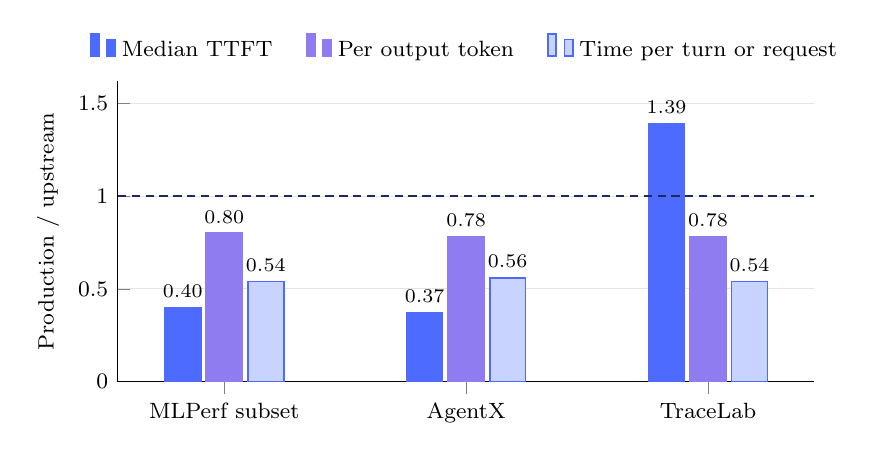
\begin{tikzpicture}
    \begin{axis}[abyss,
      width=0.86\textwidth, height=5.4cm,
      ybar=2pt, bar width=13pt, ymin=0, ymax=1.62,
      ytick={0,0.5,1,1.5},
      symbolic x coords={MLPerf,AgentX,TraceLab}, xtick=data,
      xticklabels={MLPerf subset, AgentX, TraceLab},
      enlarge x limits=0.22,
      ylabel={Production / upstream},
      nodes near coords={\pgfmathprintnumber[fixed,fixed zerofill,precision=2]{\pgfplotspointmeta}},
      nodes near coords style={font=\scriptsize},
      legend columns=3, legend style={at={(0.5,1.03)},anchor=south,/tikz/every even column/.append style={column sep=10pt}}]
      \addplot[fill=dsblue,draw=dsblue] coordinates {(MLPerf,0.40) (AgentX,0.37) (TraceLab,1.39)};
      \addplot[fill=dsviolet,draw=dsviolet] coordinates {(MLPerf,0.80) (AgentX,0.78) (TraceLab,0.78)};
      \addplot[fill=dslight,draw=dsblue] coordinates {(MLPerf,0.54) (AgentX,0.56) (TraceLab,0.54)};
      \legend{Median TTFT, Per output token, Time per turn or request}
      \draw[dsdark, densely dashed, line width=0.6pt] ({rel axis cs:0,0} |- {axis cs:MLPerf,1}) -- ({rel axis cs:1,0} |- {axis cs:MLPerf,1});
    \end{axis}
  \end{tikzpicture}
  \caption{Ratios of production to upstream in the three benchmarks; below 1 means production is faster (the dashed line is parity). All are subsets we ran ourselves, not official results; the MLPerf subset is not an MLPerf result and is not verified by MLCommons Association. The MLPerf subset is the 54 turns of 11-07, with the time per turn averaged; AgentX is the 22 requests both sides measured on 11-07, and TraceLab the 16 of 11-09, with times summed.}
  \label{fig:benchratio}
\end{figure}

\begin{table}[h]
  \centering
  \small
  \caption{Three runs of the MLPerf Agentic Inference subset (3 conversations, 54 turns, with the same input turn by turn; sampled at temperature 1.0, so output lengths differ). Not an MLPerf result and not verified by MLCommons Association (Result not verified by MLCommons Association). Between 11-07 and 11-09, production gained 0044 and 0045; between 11-09 and 11-10, 0046.}
  \label{tab:mlperf}
  \begin{tabular}{@{}l r r r r@{}}
    \toprule
     & 11-07 upstream & 11-07 prod. & 11-09 prod. & 11-10 prod. \\
    \midrule
    TTFT, median / p90 (s) & 3.99 / 15.56 & 1.60 / 4.68 & 1.61 / 4.57 & 1.37 / 4.08 \\
    Per output token, median (ms) & 25.6 & 20.5 & 20.4 & 20.4 \\
    Latency per turn, mean (s) & 32.7 & 17.5 & 16.2 & 14.2 \\
    Output tokens per turn, mean & 928 & 736 & 690 & 608 \\
    Interactive speed (\tps{}) & 28.42 & 41.96 & 42.54 & 42.94 \\
    Inline accuracy (47 turns) & 0.527 & 0.572 & 0.591 & 0.578 \\
    \bottomrule
  \end{tabular}
\end{table}

Table~\ref{tab:mlperf} shows the three runs of the MLPerf subset. Interactive speed is the total number of output tokens divided by the sum of the per-turn times, so it already accounts for the different output lengths. The inline accuracy serves only to confirm that the outputs did not go wrong: there are only 3 conversations here, the differences between runs are within sampling noise, and it cannot be compared with the accuracy threshold that MLPerf specifies. On the 22 identical AgentX requests (prompts averaging 97K tokens, 88.5\% of them from the cache), the mean time to first token (TTFT) was 4.61 vs.\ 16.73 s, the time between output tokens 19.6 vs.\ 25.0 ms, and the total request time 484 vs.\ 858 s. Computing the 65,756-token prefix cold during warm-up took 30.0 s on production and 166.7 s on upstream; with 0044, production took 20.9 s (11-09) and 20.1 s (11-10).

On TraceLab, production loses on one measure. On the 16 identical requests (prompts averaging 161K tokens), the mean TTFT was 14.07 vs.\ 33.72 s and the total request time 440 vs.\ 820 s, so production was still faster, and computing the 144K-token prefix cold also took 45.5 s on production against 358.8 s on upstream. But the median TTFT was 10.98 vs.\ 7.92 s, and the share served from the cache 76\% vs.\ 93\%. The cause lies in how this dataset synthesizes prefixes, combined with the tail merge of \S\ref{sec:tailmerge}. The data has only token counts, so the reader synthesizes the shared part in 64-token blocks from the recorded cached-prefix length. A new request shares with the previous one only up to the last full block, so every new request breaks off inside the last block of the previous user message, 6--57 tokens before the end of the previous prompt. To avoid one extra call split, the tail merge builds no checkpoint in the last 2,700 tokens, so there is no checkpoint at the start of the last user message, and the server can only fall back to a distant one, recomputing 14K--23K tokens every turn. Upstream cuts both at the start of the last user message and 2,052 tokens before the end, so it recomputes only a few hundred tokens per turn. Our own clients always append at the end, so the server continues from the end of the slot (\S\ref{sec:continue}) and never hits this case. What we could do is keep that cut for a session once a ``new request breaking off inside the previous user message'' has occurred in it; this has not been done yet.

Between 11-09 and 11-10 only 0046 went in: the MLPerf subset's median TTFT went 1.61 $\to$ 1.37 s, AgentX's on 30 identical requests 3.67 $\to$ 3.22 s, and TraceLab's on 33 identical requests 9.67 $\to$ 9.26 s. This is exactly the per-turn prefill time 0046 saves; the time between output tokens did not change. The three benchmarks agree with our own comparison: the time per output token is 0.78--0.80 of upstream's (about 20 vs.\ 25 ms), the same work takes about half the time, and cold prefill of long prompts is 5--8 times faster.

% ---------------------------------------------------------------- 12
\section{Conclusion, limitations and future directions}

On a two-GPU workstation, Abyss runs DeepSeek-V4.1-Flash (the 1017 release since 10-27) at native MXFP4 precision with a 192K context: single-stream decode in an append-only multi-turn session reaches about 52 \tps{} (at a 96K context; about 50 \tps{} per request in production); prefill takes about 14 s for a 48K-token prompt, about 27 s for a 96K-token prompt, and about 2 s per turn of a multi-turn session. With the same weights and the same launch arguments, upstream llama.cpp decoded at 39.3 against our 49.2 \tps{} in the 11-07 comparison, and its prefill of long prompts took more than 5 times as long; on subsets of three public agent benchmarks (not official results), we took about half as long as upstream for the same work. The gains come from six kinds of work: reducing computation by following the model's structure (CED-aware prefill, the sparse indexer, decode attention over only the top-k rows); placing data in a tier according to its heat (the expert cache, admission and the admission gate); keeping the CPU, DMA and both GPUs working at the same time (the miss split, expert deferral, the big-batch split and big batches from the cache, the two-GPU pipeline); cutting repeated reads and computation (the one-pass prompt tail, no longer recomputing the previous turn's answer); removing unnecessary synchronization and small overheads (stats without splitting the graph, small-kernel fusion, removing several host waits); and giving every piece of freed VRAM to the expert cache. Every item was profiled first and implemented second, and its correctness was confirmed with the tiered numerical floor, cross-checks against the official implementation and the decode-path PPL. Profiling itself can mislead: repeated generation from the same prompt and nsys node-level tracing both once led us to overestimate the gains.

\paragraph{Limitations.} The floor for decode is set by memory bandwidth: in each of layers 22--38, the CPU takes longer on the missed experts than GPU1 takes on its segment, so even if all host-memory traffic were hidden behind GPU computation, each token would still take about 15 ms (\S\ref{sec:nowtime}); the big batches of prefill are also already close to the floor of ``reading each layer's experts once''. VRAM is almost full: at peak, GPU0 has only about 0.6 GB free (which is why the display can no longer be connected to GPU0) and GPU1 about 1.4 GB, so a longer context or enabling DSpark would first require shrinking the expert cache again. The only approximation that changes the computation is expert deferral, and its difference in decode-path PPL is within the error. GPU1's link occasionally comes up at a reduced speed after a cold boot (\S\ref{sec:incidents}), and after a BIOS change the IOMMU was once turned on, making copies between the GPUs fail silently (\S\ref{sec:ddr}), so after every boot and every settings change the links and GPU-to-GPU copies must be verified first. The server has only one slot, and only that slot is saved on a restart; clients that rewrite the last user message need the checkpoint that tail merge removes (\S\ref{sec:benchmarks}). The Engram tables were reduced from the official FP8 to MXFP4 (relative error about 12\%, \S\ref{sec:formats}), and we have not directly measured how this affects task scores. On the input side, control-token strings in request text are already encoded by the official rules; the output side is not handled yet: when the model itself writes \code{</think>} or a tool-call tag with ordinary tokens, the parser still recognizes it by its text.

\paragraph{Future directions.} The first two items come from profiling and benchmarks on this machine; the others come from comparisons with DeepInfer~\cite{deepinfer}, the inference framework DeepSeek open-sourced, and with vLLM:
\begin{itemize}
  \item \textbf{Staging only the experts that big batches use.} About 4.7 GB of GPU0's compute buffer is the staging area for uploading the experts of layers 22--39 for big prefill batches, sized for whole expert tensors. Staging only the experts in use would free about 3 GB on GPU0; moving some of the experts of layers 13--21 there and giving the VRAM freed on GPU1 to the cache should make decode about 0.5 ms faster per token (\S\ref{sec:tp}).
  \item \textbf{Keeping that split point for sessions that rewrite messages.} Once a session has shown ``a new request diverging inside the previous user message'', keeping for that session the checkpoint that tail merge removes would stop replays such as TraceLab from losing to upstream on time to first token (\S\ref{sec:benchmarks}).
  \item \textbf{Sparse prefill attention.} Chunking the indexer by query is already done (\S\ref{sec:gpu0cache}). DeepInfer's prefill attention also takes only the SWA window and the top-512 rows through an index table; the fork still builds a dense mask for every layer that uses the indexer and has flash attention sweep all compressed positions with that mask. Rewriting it this way would remove the mask and might win back the 4--8\% by which chunking slows long prefills. This item introduces no approximation.
  \item \textbf{Bounded replay in the decoder.} When DeepInfer prefills in production, the decoder layers compute only the last 140 tokens of the whole prompt, with SWA truncated to within that span; this is an approximation. Our CED is an exact cascade, and we measured that in each agent turn each of layers 22--38 still computes about 1,000 tokens (\S\ref{sec:bigcache}). With bounded replay, both the experts needed and the tokens computed would drop, and the two compromises \code{0015} and \code{--checkpoint-min-step 32768} could also be dropped; the difference the approximation introduces would first have to be measured with KLD and PPL.
  \item \textbf{Resuming at any position.} vLLM's approach for DSV4 keeps a copy of the compressor state every 256 positions within one call, so any 256 boundary in a prompt can serve as a checkpoint without splitting the call; DeepInfer instead restores the sliding-window state at any 128-aligned position by recomputing the last 128 tokens. Either would remove several checkpoint-related compromises, but both require changing the fork's DSV4 cache management, the most work of all these items; judging from the production logs, it would currently save only about 2 s each time (\S\ref{sec:prefixcache}).
  \item \textbf{DSpark speculative decoding.} With vLLM on 4 RTX PRO 6000 cards and a single stream, enabling it raised chat from 83.6 to 146.8 \tps{} and agent workloads from 82.2 to 130.5 \tps{}~\cite{infatoshi}; DeepInfer verifies only part of the draft, chosen by confidence. On this machine it is worth redoing only if all three of these hold: the verification batch can also use the single-token optimizations, the draft model processes only the tail of the prompt, and about 10 GB of VRAM can be freed without cutting the cache (\S\ref{sec:notadopted}).
  \item \textbf{Control tokens on the output side.} The fork's parser has the token IDs but recognizes tags by their text; if it used the IDs, a \code{</think>} or tool-call tag that the model writes with ordinary tokens would no longer be taken as real.
\end{itemize}

\begin{thebibliography}{99}
\bibitem{v41} DeepSeek-AI. DeepSeek-V4.1-Flash: Pushing the Limits of KV Cache Compression. 2026. \url{https://huggingface.co/deepseek-ai/DeepSeek-V4.1-Flash}
\bibitem{mxllama} mxxm-t. mx-llama.cpp and the MXFP4 GGUF of DeepSeek-V4.1-Flash. \url{https://huggingface.co/mxxm-t/DeepSeek-V4.1-Flash-GGUF}
\bibitem{diffbot} diffbot. DeepSeek-V4.1-Flash-EXL3-3bpw-2x-RTX-PRO-6000. \url{https://huggingface.co/diffbot/DeepSeek-V4.1-Flash-EXL3-3bpw-2x-RTX-PRO-6000}
\bibitem{strata} Strata: local MoE inference with a three-tier division of labor. \url{https://github.com/Niko1221/Strata}
\bibitem{v411017} DeepSeek-AI. DeepSeek-V4.1-Flash-1017. 2026. \url{https://huggingface.co/deepseek-ai/DeepSeek-V4.1-Flash-1017}
\bibitem{deepinfer} DeepSeek-AI. DeepInfer and its deployment Q\&A (\code{doc/inference\_deployment\_qa.md}). 2026. \url{https://github.com/deepseek-ai/deepinfer}
\bibitem{nvfp4} NVIDIA. DeepSeek-V4.1-Flash-NVFP4. 2026. \url{https://huggingface.co/nvidia/DeepSeek-V4.1-Flash-NVFP4}
\bibitem{recipe} DeepSeek-AI. DeepSeek Recipe. 2026. \url{https://github.com/deepseek-ai/deepseek-recipe}
\bibitem{infatoshi} Infatoshi. DeepSeek-V4.1-Flash-1017-MXFP4-uncensored, the DSpark ablation in its model card. 2026. \url{https://huggingface.co/Infatoshi/DeepSeek-V4.1-Flash-1017-MXFP4-uncensored}
\bibitem{ktrans} kvcache-ai. KTransformers: DeepSeek-V4-Flash. 2026. \url{https://github.com/kvcache-ai/ktransformers/blob/main/doc/en/DeepSeek-V4-Flash.md}
\bibitem{llamacpp} ggml-org. llama.cpp. \url{https://github.com/ggml-org/llama.cpp}
\bibitem{mlperf} MLCommons. MLPerf Agentic Inference (\code{mlcommons/endpoints}, \code{examples/10\_Agentic\_Inference}). 2026. \url{https://github.com/mlcommons/endpoints}
\bibitem{agentx} SemiAnalysis. InferenceX v3: AgentX. 2026. \url{https://inferencex.semianalysis.com/blog/agentx-inferencexv3-does-cuda-moat}
\bibitem{tracelab} uw-syfi. TraceLab: traces of real Claude Code and Codex sessions. 2026. \url{https://github.com/uw-syfi/TraceLab}
\bibitem{vllm} vLLM. DeepSeek V4 in vLLM; the Automatic Prefix Caching design document. 2026. \url{https://vllm.ai/blog/deepseek-v4}
\bibitem{sglang} L. Zheng et al. SGLang: Efficient Execution of Structured Language Model Programs. arXiv:2312.07104.
\end{thebibliography}

\newpage
\appendix

\section{Patch list}

All of Abyss's changes are kept as patches in the repository's \code{mx-llama.cpp/} directory, based on mx-llama.cpp commit \code{c4d12e2} and applied in numbered order. Production uses everything up to \code{0046}; of these, \code{0024}, \code{0031} and \code{0037} are not deployed and the timing in \code{0033} is off by default, and none of them has any effect unless its switch is set. The prototype of tensor parallelism for layers 0--19 is not part of this sequence; it is saved separately as \code{experiments/tp-layers.diff} (\S\ref{sec:tp}).

\begin{table}[h]
  \centering
  \small
  \begin{tabularx}{\textwidth}{@{}l X l@{}}
    \toprule
    Patch & Purpose & Switch \\
    \midrule
    0001 & Expert hit statistics in the server & \code{ABYSS\_EXPERT\_STATS} \\
    0002 & V4.1 tool-call tags (DSML, with a leading space in the tag names) & --- \\
    0003 & CED-aware prefill: decoder layers compute the FFN only for visible tokens & \code{ABYSS\_CED\_PREFILL=1} \\
    0004 & Engram prefetch for whole batches & \code{ABYSS\_ENGRAM\_PREFETCH=8} \\
    0005 & CED-aware prefill: attention also computes only the subset & Same as 0003 \\
    0006 & V4.1 sparse attention indexer & \code{ABYSS\_DSV41\_INDEXER=1} \\
    0007 & \code{llama-abyss-dump}: dumps compute-graph tensors for cross-checks & --- \\
    0008 & Attention in single-token decode takes only the top-k rows & \code{ABYSS\_DSV41\_DECODE\_GATHER=1} \\
    0009 & Expert cache misses split by heat between upload and the CPU & \code{ABYSS\_MOE\_CPU\_MISS=1} \\
         & & \code{ABYSS\_MOE\_ADMIT=0.3} \\
    0010 & Fixes the unallocated CED row map and the duplicated all-zero slot in the miss split & --- \\
    0011 & Fixes the unallocated candidate-block input & --- \\
    0012 & Prompt cache selection by the number of directly usable tokens & --- \\
    0013 & Fixes the scheduler clearing manually assigned backends when estimating VRAM & --- \\
    0014 & Big-batch split of prefill onto the CPU & \code{ABYSS\_MOE\_BIG\_SPLIT=1} \\
    0015 & One-pass prompt tail; the CED margin follows \code{n\_rs\_seq} & \code{ABYSS\_CKPT\_TAIL\_MERGE=2700} \\
         & & \code{ABYSS\_CED\_ALIGN=1} \\
    0016 & Decode stats: one line every N decoded tokens with the time per token, hit rate, number of experts uploaded and computed on the CPU, and page faults & \code{ABYSS\_DECODE\_STATS=100} \\
    0017 & Saves the slot into the in-memory cache before a request that shares only the beginning takes it over; the checkpoint thinning interval is set separately & \code{ABYSS\_SLOT\_SAVE\_LOST} \\
         & & \code{ABYSS\_CKPT\_THIN\_STEP=8192} \\
    0018 & Encodes chat prompts by the official Recipe's rules: only the control tokens the template writes are encoded as IDs & \code{ABYSS\_PLAIN\_INPUT=1} \\
    0019 & Compute-graph VRAM: all-zero tensors allocated only when used, no queries computed for layers without query rows; every allocation can be logged & \code{GGML\_ALLOC\_TRACE=1} \\
    0020 & Prefill indexer scoring and attention chunked by query & \code{ABYSS\_DSV41\_IDX\_CHUNK=512} \\
    0021 & llama-bench reads the expert cache size from an environment variable & \code{LLAMA\_ARG\_MOE\_CACHE\_MIB} \\
    0022 & Statistics for big prefill batches: the experts in each batch and how many of them are already cached & \code{ABYSS\_MOE\_BIG\_STATS=1} \\
    0023 & In big prefill batches, experts already in the cache are computed on the GPU that holds the cache & \code{ABYSS\_MOE\_BIG\_CACHE=1} \\
    \bottomrule
  \end{tabularx}
\end{table}

\begin{table}[h]
  \centering
  \small
  \begin{tabularx}{\textwidth}{@{}l X l@{}}
    \toprule
    Patch & Purpose & Switch \\
    \midrule
    0024 & Predicts experts during decode with the next layer's router gate and uploads them early (not deployed) & \code{ABYSS\_MOE\_PREFETCH=K} \\
    0025 & Expert deferral: experts computed on the CPU are added back to the residual one layer later; the scheduler sends small inputs asynchronously & \code{ABYSS\_MOE\_DEFER=1} \\
    0026 & Expert stats copy back the selections asynchronously after each ubatch instead of splitting the graph & With expert stats \\
    0027 & Split-K for the hyper-connection mixing coefficients & \code{ABYSS\_HC\_KSPLIT=1} \\
    0028 & Issues \code{MADV\_WILLNEED} early during decode for the Engram rows to be fetched & \code{ABYSS\_ENGRAM\_DECODE\_PREFETCH=1} \\
    0029 & Vectorized exp for \code{dist} sampling & \code{ABYSS\_DIST\_VEC=1} \\
    0030 & Cache eviction by decayed heat, and an admission gate; experts computed on the CPU do not read the zero slot & \code{ABYSS\_MOE\_EVICT=cold} \\
         & & \code{ABYSS\_MOE\_ADMIT\_GATE=1} \\
         & & \code{ABYSS\_MOE\_SKIP\_ZERO=1} \\
    0031 & Uploaded experts deferred too (not deployed) & \code{ABYSS\_MOE\_DEFER\_UPLOAD=1} \\
    0032 & Small-kernel fusion for hyper-connections and for KV assembly in single-token attention & \code{ABYSS\_HC\_FUSE=1} \\
         & & \code{ABYSS\_GATHER\_FUSE=1} \\
    0033 & Per-step timing in the server (off by default) & \code{ABYSS\_SERVER\_STATS=N} \\
    0034 & With a single output, each GPU computes half of the output head & \code{ABYSS\_HEAD\_SPLIT=0.5} \\
    0035 & Sampling fast path: samples directly from the logits & \code{ABYSS\_SAMPLE\_FAST=1} \\
    0036 & Several rows per block for the tail of matrix-vector products; a dedicated pool for the q8\_1 cache & \code{ABYSS\_MMVQ\_TAIL=1} \\
    0037 & The q8\_1 cache's dedicated pool holds only small entries (not deployed) & \code{ABYSS\_Q8\_1\_CACHE\_LEG=1} \\
    0038 & Large CUDA graphs launched in two parts & \code{ABYSS\_GRAPH\_CHUNK=128} \\
    0039 & NVMe keep-alive during decode & \code{ABYSS\_ENGRAM\_KEEPALIVE\_MS=4} \\
    0040 & Output head loaded only as two halves, without keeping the whole tensor & \code{ABYSS\_HEAD\_SPLIT\_ONLY=1} \\
    0041 & Saves a checkpoint every 256 generated tokens; logs where each request resumes from & \code{ABYSS\_GEN\_CKPT=256} \\
    0042 & Checkpoint window of 0 for V4.1 (following upstream) & --- \\
    0043 & CUDA graphs not cleared after idling (following upstream) & --- \\
    0044 & Two-GPU pipeline for long-prompt prefill & \code{ABYSS\_OVERLAP=1} \\
    0045 & Checkpoint splitting counts the checkpoint at the start of the call; logs each request's calls & \code{ABYSS\_CKPT\_COUNT\_START=1} \\
    0046 & No longer makes the host wait before copying weights that live in host memory & \code{ABYSS\_WEIGHT\_NOWAIT=1} \\
    \bottomrule
  \end{tabularx}
\end{table}

\section{Reproduction}

The launch command for the production configuration is below. It needs a build with \code{0001}--\code{0046} applied; in the BIOS, memory is set to EXPO I + DDR5-6000 and the IOMMU is off (\S\ref{sec:ddr}). The two GGML environment variables are required, and \code{CUDA\_SCALE\_LAUNCH\_QUEUES=4x} goes with \code{0044}. The weights are the GGUF converted from the official 1017 release with \code{v41convert.py} (\S\ref{sec:w1017}), and the template is \code{deepseek-v4.1.jinja} from the repository; the repository's \code{restart-server.sh} also adds slot save and restore, expert stats and decode stats:

\begin{small}
\begin{verbatim}
GGML_CUDA_Q8_1_CACHE=0 GGML_CUDA_MMQ_PREC=q8 GOMP_SPINCOUNT=100000000 \
CUDA_SCALE_LAUNCH_QUEUES=4x \
ABYSS_CED_PREFILL=1 ABYSS_ENGRAM_PREFETCH=8 ABYSS_DSV41_INDEXER=1 \
ABYSS_DSV41_IDX_CHUNK=512 ABYSS_DSV41_DECODE_GATHER=1 \
ABYSS_MOE_CPU_MISS=1 ABYSS_MOE_ADMIT=0.3 ABYSS_MOE_BIG_SPLIT=1 \
ABYSS_MOE_BIG_CACHE=1 ABYSS_PLAIN_INPUT=1 \
ABYSS_CKPT_TAIL_MERGE=2700 ABYSS_CED_ALIGN=1 ABYSS_CKPT_THIN_STEP=8192 \
ABYSS_MOE_DEFER=1 ABYSS_HC_KSPLIT=1 ABYSS_ENGRAM_DECODE_PREFETCH=1 \
ABYSS_DIST_VEC=1 ABYSS_MOE_EVICT=cold ABYSS_MOE_ADMIT_GATE=1 \
ABYSS_MOE_SKIP_ZERO=1 ABYSS_HC_FUSE=1 ABYSS_GATHER_FUSE=1 \
ABYSS_HEAD_SPLIT=0.5 ABYSS_HEAD_SPLIT_ONLY=1 ABYSS_SAMPLE_FAST=1 \
ABYSS_MMVQ_TAIL=1 ABYSS_GRAPH_CHUNK=128 ABYSS_ENGRAM_KEEPALIVE_MS=4 \
ABYSS_GEN_CKPT=256 ABYSS_OVERLAP=1 ABYSS_CKPT_COUNT_START=1 \
ABYSS_WEIGHT_NOWAIT=1 \
llama-server -m DeepSeek-V4.1-Flash-1017-MXFP4-00001-of-00012.gguf \
  -ngl 99 -sm layer -ts 12/29 -fa 1 -lm dio -c 196608 -b 65536 -ub 2048 \
  -ot "blk\.(2[2-9]|3[0-9])\.ffn_(gate|up|down)_exps\.=CPU" \
  -ot "blk\.12\.ffn_(gate|up)_exps\.=CUDA0" \
  -t 16 -np 1 --moe-cache-mib 21100 --checkpoint-min-step 32768 \
  --jinja --chat-template-file deepseek-v4.1.jinja --no-reasoning-preserve \
  --temp 1.0 --top-p 1.0 --top-k 0 --min-p 0
\end{verbatim}
\end{small}

The evaluation scripts are in the repository's \code{tools/eval/}; they are copied to the machine and run there, and the server must be stopped before running them; see Table~\ref{tab:tools}. The scripts for running the three public benchmarks are in the repository's \code{benchmark/}.

\begin{table}[tp]
  \centering
  \footnotesize
  \caption{Evaluation scripts.}
  \label{tab:tools}
  \begin{tabularx}{\textwidth}{@{}l X@{}}
    \toprule
    Script & Purpose \\
    \midrule
    \multicolumn{2}{@{}l}{\textit{October}} \\
    \code{kl.sh} & Saves baseline logits and compares KLD \\
    \code{bench.sh} & Decode and prefill speed \\
    \code{prefill-warm.sh} & Server prefill with a warm cache \\
    \code{profile-prefill.sh}, \code{profile-decode.sh} & nsys profiles of prefill and decode \\
    \code{dump-indexer.sh}, \code{indexer\_oracle.py} & Single-layer cross-check of the sparse indexer \\
    \code{decode-gather.sh}, \code{decode\_attn\_oracle.py} & float64 cross-check of decode attention \\
    \code{engram-cold.sh}, \code{engram-share.sh} & Cost of cold Engram reads and Engram's share of the time \\
    \code{m2-cpu-miss.sh} & Admission-ratio sweep for the miss split \\
    \code{agent-turns.sh} & Multi-turn agent sessions \\
    \code{decode\_modes.sh} & Decode in a long append-only session; \code{CAPTURE=1} profiles it \\
    \code{prefill-sizes.sh} & Prefill of new prompts of several lengths \\
    \code{ctx-size.sh} & Peak VRAM, long-prompt prefill and passkey retrieval for each context configuration \\
    \code{slot-takeover.sh} & How much the main conversation can still reuse after a request that shares only the beginning takes the slot \\
    \code{template\_check.py} & Cross-checks the chat template against the official \code{encoding.py} \\
    \code{special\_check.py} & Token-by-token cross-check of chat-prompt encoding against the official Recipe's rules \\
    \code{align\_sweep.py} & Boundary sweep over every remainder of the call length divided by 2,048 \\
    \code{experts5.sh} & KLD and decode speed of 5 experts per token versus 6 \\
    \code{dspark.sh}, \code{dspark\_code.py} & Speed, acceptance rate and VRAM of DSpark speculative decoding \\
    \code{alloc-trace.sh}, \code{alloc\_peak.py} & Which tensors are present at the compute buffer's peak \\
    \code{idx-chunk.sh} & Cross-check, VRAM and long prompts for indexer chunking \\
    \code{cache-decode.sh}, \code{gpu0-experts.sh} & Decode with different expert cache sizes and tensor placements \\
    \code{admit-sweep.sh}, \code{threads-sweep.sh} & Sweeps of the admission ratio and the CPU thread count \\
    \code{quick-knobs.sh} & CUDA graphs, graph optimization and chunk size \\
    \code{profile-prod.sh}, \code{nsys\_layer.py} & Profiles decode and one prefill turn with the production settings; prints the timeline of one layer \\
    \code{big-coverage.sh}, \code{big-cache.sh} & Cache coverage of big batches; comparison with \code{0023} off and on \\
    \code{std-bench.sh} & Standard measurements with llama-bench and AIPerf \\
    \midrule
    \multicolumn{2}{@{}l}{\textit{November}} \\
    \code{cache-gate.sh} & Compares switches on the production settings: numerics, session speed, cache statistics \\
    \code{defer.sh}, \code{greedy\_kl.py} & Expert deferral comparison; greedy generation on several corpus segments, top-20 KL over the common prefix \\
    \code{defer-ppl.sh}, \code{nll\_compare.py} & Forced decoding; paired token-by-token comparison of decode-path PPL \\
    \code{prod-decode-profile.sh} & Profiles decode with the production settings: per layer, per kernel, CUDA graph launches \\
    \code{expert-trace.sh}, \code{cache\_policy.py} & Dumps decode routing; compares cross-layer prediction and cache policies offline \\
    \code{engram-decode.sh}, \code{engram\_reads.c} & Profile of Engram disk reads during decode; ways to read cold rows and the first read after idle \\
    \code{host-profile.sh} & Off-CPU call stacks and durations of the main thread during decode \\
    \code{vram-peak.sh} & Peak VRAM on both GPUs after loading and after several workloads \\
    \code{sample-fast.sh}, \code{seeded\_tokens.py} & Token-by-token cross-check of sampling with fixed seeds \\
    \code{gen-ckpt.sh}, \code{prefix\_reuse.py} & Comparison of resuming after the previous answer; slot reuse statistics from server logs \\
    \code{prefill-pipe.sh}, \code{big-pipe.sh} & Profiles of long-prompt prefill and of one agent turn's prefill, broken down by GPU \\
    \code{upstream-bench.sh}, \code{upstream-ppl.sh} & Compares upstream and production in one production stop; PPL on both paths \\
    \code{tp-measure.sh}, \code{tp-proto.sh} & Two-GPU all-reduce latency; comparison of the tensor-parallel prototype \\
    \code{gpu-bw.sh}, \code{gpu\_memtest.cu} & Checks links, bandwidth and GPU-to-GPU copies after a boot or a BIOS change \\
    \code{precision\_audit.py} & Class-by-class check of the GGUF tensors against the official checkpoint \\
    \code{benchmark/run.sh}, \code{compare-runs.sh} & Subsets of the three public benchmarks; comparison of two runs \\
    \bottomrule
  \end{tabularx}
\end{table}

The conversion scripts are in \code{tools/convert/}: \code{v41convert.py verify} samples the original weights and compares them against the template, \code{convert} does the conversion, and \code{check} checks the output.

\clearpage
\section{Glossary}
\label{sec:glossary}

Grouped by topic. Where the same word means different things in different contexts (such as ``decoder layers'' and ``decode'', or server slots and expert cache slots), the entries explain each sense separately.

\setlist[description]{font=\normalfont\bfseries,leftmargin=0pt,itemsep=0.25em}

\subsection*{Model structure}
\begin{description}\small
  \item[MoE (mixture of experts)] Each layer has many feed-forward networks (experts), and each token is computed by only the few of them that the router picks. V4.1-Flash has 384 routed experts per layer and picks 6 per token, plus 1 shared expert computed for every token.
  \item[Router (gate)] The small matrix in each layer that scores the 384 experts and selects the top 6; the expert IDs it selects decide which expert weights this step must read.
  \item[CED (encoder-decoder structure)] V4.1 divides its 40 layers into a causal encoder of the first 20 layers (layers 0--19) and a decoder of the last 20 layers (layers 20--39). Layer 20 uses the encoder's output to produce the global KV shared by all decoder layers; the decoder layers' own hidden states are visible to other tokens only through a 128-token sliding window. So earlier tokens in a prompt do not need to go through all of the decoder layers, which is the basis of CED-aware prefill.
  \item[Encoder layers, decoder layers] Layers 0--19 and layers 20--39 respectively, a division in the model structure; not the same thing as ``decode'' (generating tokens one by one) in the inference process below.
  \item[Sliding-window attention (SWA)] Each token sees only the KV of itself and the preceding 127 positions (128 in total).
  \item[Compressed attention, compression ratio] The KV of every 2 tokens, or of every 1 token, is compressed into one row, and long-range attention sees only the compressed rows. Layers 0--1 have only the sliding window, layers 2--19 have a compression ratio of 2, and layers 20--39 a ratio of 1. Compressed KV is written only at layers 2, 8, 14 and 20 (the KV source layers) and reused by the layers after them.
  \item[Global KV] The compressed KV produced by layer 20's compressor and shared by all decoder layers.
  \item[Sparse indexer (lightning indexer)] Scores all compressed positions with 32-head, 128-dimensional FP4 queries and keys and picks the top 512 positions for each query; attention sees only these positions and the sliding window, about 640 rows in total. Layers 2, 8, 14, 20, 24, 28, 32 and 36 are index source layers; the other layers reuse the result of the nearest index source.
  \item[Candidate blocks] Layer 20 picks 2,048 blocks of 8 compressed positions each, and layers 24--36 reselect the top 512 only within these blocks.
  \item[Hyper-connections (hc)] The V4 series' extension of residual connections: the hidden state keeps 4 streams, which are mixed with learned coefficients and written back before and after each layer's attention and feed-forward network. In decode they bring many small kernels.
  \item[Engram] V4.1's lookup module: layers 1 and 14 hash the n-grams of the last 2--4 tokens and fetch rows from two large tables of about 384 million rows each. The tables are large (about 189 GiB in the official FP8), but each token reads only a few dozen rows, so they can be kept on NVMe.
  \item[DSpark] V4.1's built-in draft model of about 14B for speculative decoding: 3 layers, each picking 3 of 128 experts, producing 5 tokens at a time, reading the hidden states of the main model's layers 37--39, and predicting with a confidence head the probability that each draft token is accepted. Tried on this machine and not adopted for now (\S\ref{sec:notadopted}).
\end{description}

\subsection*{Numeric formats and quantization}
\begin{description}\small
  \item[MXFP4] 4-bit floating point (E2M1) with an 8-bit power-of-two scale (E8M0) shared by every 32 elements, 4.25 bits per weight on average. The native format of V4.1's routed experts.
  \item[FP8, BF16, F16, F32] 8-, 16-, 16- and 32-bit floating point. The dense weights and the Engram tables of the official checkpoint are FP8; the KV cache uses F16.
  \item[Q8\_0] llama.cpp's 8-bit integer format with one F16 scale per 32 elements, 8.5 bits on average. The dense weights in the GGUF use this format.
  \item[W4A8, W4A4] Matrix-multiplication precision: 4-bit weights, with activations quantized to 8 or 4 bits. The official reference implementation is W4A8; the fork's prefill on Blackwell defaults to W4A4, and we switch it back to 8 bits with \code{GGML\_CUDA\_MMQ\_PREC=q8}.
  \item[bpw] Average number of bits per weight. Plan A compresses the experts from about 4.25 bpw to 3.0 bpw.
  \item[EXL3] ExLlamaV3's quantization format, used by the public recipe for Plan A.
  \item[GGUF] llama.cpp's model file format. This report first used the MXFP4 GGUF converted by mxxm-t, and since 10-27 the 1017 version that we converted ourselves in the same format; both are 12 shards and 383 GiB.
\end{description}

\subsection*{Inference process}
\begin{description}\small
  \item[Prefill] Processes the whole prompt at once, writing the KV and computing the distribution of the first token. Many tokens are computed together, so it is limited mainly by compute and by the total amount of weights read.
  \item[Decode] Generates one token at a time. Each step must read all the weights it uses once, so it is limited mainly by bandwidth.
  \item[tok/s] Tokens per second: for prefill, the prompt tokens processed per second; for decode, the tokens generated per second.
  \item[KV cache] The keys and values of the positions already processed, which later tokens read in attention. V4.1's KV is small: each position has only one 512-dimensional head, and it is compressed as well.
  \item[llama\_decode call, ubatch] The server groups the tokens to be processed into one \code{llama\_decode} call (capped by \code{-b}; this report uses 65536); a call is further cut into ubatches of at most 2,048 tokens (\code{-ub}), and each ubatch runs the compute graph from beginning to end.
  \item[Checkpoint] The DeepSeek V4 cache cannot roll back to an intermediate position. At certain positions the server saves the complete state at that moment (the sliding window and the compressor state); a later request that diverges from the cache only after such a position is restored from the checkpoint instead of being computed from the start.
  \item[Prompt cache] The server keeps the state of processed prompts (together with their checkpoints) in host memory and reuses it directly when the next request has the same prefix.
  \item[Server slot] The number of sessions the server serves at the same time (\code{-np}); this report uses 1. Unrelated to the slots of the expert cache.
  \item[Rollback ring (n\_rs\_seq)] A small rollback capacity for speculative decoding that can undo the last few tokens; it is 0 when speculative decoding is off, and the cache can then only roll back to a checkpoint.
  \item[Speculative decoding] A small model first guesses several tokens, then the large model verifies them in one pass, and the correctly guessed part is accepted directly.
  \item[Chat template] The rules for assembling multi-turn messages, tool definitions and tool results into the token sequence the model sees. V4.1's official rules are in \code{encoding/encoding.py}; the server implements them as a Jinja template, which must match them character for character (\S\ref{sec:template}).
  \item[Control token] A special token in the chat template that marks roles and structure, such as \ctok{<｜User｜>}, \ctok{<｜Assistant｜>} and \code{</think>}. When the same strings appear in request text, they must be encoded as ordinary text (\S\ref{sec:special}).
  \item[temperature, top\_p] Sampling parameters: temperature adjusts how sharp the probability distribution is, and top\_p samples only among the candidates whose cumulative probability reaches p. The 1017 release recommends 1.0 for both, that is, sampling from the model's own distribution.
  \item[Bounded replay] DeepInfer's approach: when the sliding-window state has to be rebuilt, it recomputes only the last 128 tokens, with the attention window also truncated to within that span, giving an approximate SWA KV; the decoder layers' prefill likewise computes only the last 140 tokens.
  \item[temperature 0 (greedy)] Takes the most probable token at each step, so the same input always gives the same output; suited to cross-checks.
\end{description}

\subsection*{Abyss scheduler}
\begin{description}\small
  \item[Plan A, Plan B] Plan A quantizes the experts to 3.0 bpw and uses two-GPU tensor parallelism in vLLM (TP2); it is below native 4-bit and has not been considered since 11-04. Plan B keeps native MXFP4 and uses a layer split in mx-llama.cpp; it is the main line of this report.
  \item[Tensor parallelism, Meta device, all-reduce] Tensor parallelism splits a layer's weights across the two GPUs so that both compute at the same time, and after each layer the partial sums from the two sides are added together (all-reduce). The fork implements this with a Meta device spanning both GPUs; we had the first 20 layers use it while the remaining layers kept the layer split, and got as far as a prototype (\S\ref{sec:tp}).
  \item[Layer split] \code{-sm layer -ts 12/29}: GPU0 holds layers 0--11 in full, GPU1 holds the dense parts of layers 12--39 and the experts of layers 12--21, and the experts of layers 22--39 are in host memory.
  \item[Pinned host memory (CUDA\_Host)] Host memory that the operating system does not swap out and that the GPUs can read directly by DMA; the experts of layers 22--39 (121 GiB) are kept here.
  \item[Expert cache, bank, slot] A region of VRAM set aside on GPU1 (the bank), divided into slots that each hold one expert: 14 GB and about 780 slots with a 128K context; with a 192K context, at first 12 GB and about 670, then 20.5 GB and about 1,140 from 10-28, and 21.1 GB and about 1,170 from 11-07. Each layer has a table that maps expert IDs to slot numbers.
  \item[Hit, miss, hit rate] An expert selected by a token that is already in the cache is a hit; otherwise it is a miss. The hit rate is counted per ``token × expert''. In real sessions it is about 65--81\%.
  \item[LRU] Least recently used: when the cache is full, the expert that has gone unused the longest is replaced first.
  \item[Admission, heat] Not every missed expert goes into the cache: a set fraction of them (0.3 since 10-28), chosen by decayed heat (multiplied by 0.99 per layer per step), is uploaded into the cache, and the rest are computed by the CPU.
  \item[Admission gate, cold eviction (0030)] A miss is put into the cache only if it is hotter than the expert it would displace; the one displaced is the slot with the lowest decayed heat, no longer the least recently used one.
  \item[Expert deferral (0025)] During decode, the experts of layers 22--38 that are handed to the CPU are not merged into that layer's output; instead they are added to the residual with that layer's coefficients before the next layer's attention. The residual itself is exact; the only approximation is that the next layer's attention does not see this part. The benefit is that GPU1 can go on to the next layer's attention while the CPU computes these experts.
  \item[Two-GPU pipeline (0044)] During long-prompt prefill, GPU0 computes layers 0--11 of the next ubatch while GPU1 computes the later layers of the current one.
  \item[Generation checkpoints (0041)] Checkpoints saved every 256 tokens while an answer is generated; when the previous turn's answer no longer matches after re-tokenization, the server falls back to one of these instead of to the end of the previous turn's prompt.
  \item[Miss split (0009)] During decode, the missed experts are split into two paths processed at the same time: some are uploaded into GPU1's cache and computed there, and the rest are computed by the CPU directly from the weights in host memory, so each expert is read from memory only once.
  \item[Big-batch split (0014)] In prefill batches of more than 32 tokens, the experts assigned few tokens are handed to the CPU, and the rest are uploaded to GPU0 as usual.
  \item[CED-aware prefill (0003, 0005)] The decoder layers compute the feed-forward network and attention only for the tokens that later tokens can still see through the sliding window; all KV is still written as usual.
  \item[Big batches from the cache (0023)] In big prefill batches, experts already in the cache are computed directly on GPU1 from their slots, and the rest are split between the CPU and uploads to GPU0 as before; the three paths run at the same time.
  \item[Indexer chunking (0020)] During prefill, the sparse indexer's scoring and attention compute only one chunk of queries at a time (512 in production), so the compute buffer no longer grows with the whole ``ubatch × context''.
  \item[One-pass prompt tail (0015)] Keeps the server from splitting the last part of the prompt into several calls and makes the last ubatch of a call a full one, so that the decoder layers' experts are read only once where possible.
  \item[Compute graph, split] ggml represents one forward pass as a compute graph and then cuts it into segments (splits) by the device of each operator; each split runs on one backend (CPU, GPU0 or GPU1), with data copies and synchronization between splits.
  \item[MMQ, MMVQ] Quantized matrix-multiplication kernels in CUDA: MMQ for batches of more than 8 tokens (prefill), MMVQ for 1--8 tokens (decode).
  \item[CUDA graph] Records a sequence of kernels as a single submission, reducing the overhead of launching them one by one. Large graphs with many nodes are cut in two after the 128th node, and the second part is submitted while the first runs (0038).
  \item[flash attention] An attention kernel that computes attention block by block without materializing the full attention matrix.
\end{description}

\subsection*{Evaluation methods}
\begin{description}\small
  \item[Cross-check] Comparing, item by item on the same input, the output after a change with the output before it or with a reference implementation.
  \item[KLD (KL divergence)] The difference between the probability distributions that two configurations output at each position, averaged; 0 means identical. This report computes it with llama.cpp's \code{llama-perplexity}.
  \item[Numerical floor] The KLD produced even by changes that do not alter the semantics (a different kernel, ubatch size or compute device). About 0.0005 when a change touches only the decoder layers, and 0.005--0.01 when it passes through the encoder layers (\S\ref{sec:floors}).
  \item[Top-1 agreement] The fraction of positions where the most probable token is the same under both configurations.
  \item[top-20 KL] KL estimated only from the probabilities of the top 20 candidates the server returns; used for cross-checks on the single-token decode path.
  \item[PPL (perplexity)] The model's average ``surprise'' at a piece of text; lower is better.
  \item[Reference implementation (oracle)] A PyTorch implementation we wrote following the official \code{inference/model.py}; it recomputes layer by layer on the same input to check each step of the fork.
  \item[nsys] NVIDIA Nsight Systems, which records a timeline of GPU kernels, copies and CUDA calls; used to profile where each token's time goes. Node-level tracing of CUDA graphs shows every kernel but inflates graph launches about 3 times; to look at launches and idle time, use whole-graph tracing (\S\ref{sec:profiling}).
  \item[Decode stats (0016)] One line in the server log every 100 decoded tokens: time per token, expert cache hit rate, the number of experts hit, uploaded and handed to the CPU per token, and disk page faults. They exclude the wrap-up and sampling after \code{llama\_decode} returns, so they are about 1 ms lower than the per-token time computed per request.
  \item[Forced-decoding PPL] After the prompt, a reference text is fed in one token at a time and the negative log-likelihood of each token on the decode path is recorded; two configurations are compared pairwise. It reflects changes to single-token decode better than batch PPL does (\S\ref{sec:forcedppl}).
  \item[Fixed seed] Fixing the random seed when sampling at temperature 1.0, so that two configurations generate the same session from the same input and the cache hit rate no longer fluctuates with sampling (\S\ref{sec:seeds}).
  \item[MLPerf Agentic, AgentX, TraceLab] Three public agent inference benchmarks, from MLCommons, SemiAnalysis and the University of Washington respectively. This report runs subsets of them with a single slot and concurrency 1, only to compare production with upstream; none of them are official results, and the MLPerf one is not an MLPerf result and is not verified by MLCommons Association (\S\ref{sec:benchmarks}).
  \item[llama-bench, AIPerf] llama.cpp's bundled benchmark program (pp measures prefill, tg measures generation) and NVIDIA's load-testing tool for inference serving (measuring time to first token and time per token); this report uses them for standard measurements (\S\ref{sec:stdbench}).
  \item[stressapptest] Google's memory stress test, which repeatedly writes, reads and verifies large blocks of memory; used to confirm that there are no errors after raising the memory frequency.
\end{description}

\subsection*{Hardware and system}
\begin{description}\small
  \item[PCIe 5.0 x8, Gen3/4/5] The link between a GPU and the host: the generation sets the rate of each lane, and x8 means 8 lanes. Gen5 x8 measured about 28.9 GB/s; when link training fails at boot, the link falls back to Gen4 or Gen3.
  \item[P2P] Direct copies between the two GPUs; on this machine they are forwarded through the CPU, at about 27.7 GB/s in one direction.
  \item[MT/s, dual channel] The memory's transfers per second and its number of channels, which together set the theoretical bandwidth: dual channel at 3600 MT/s gives about 57.6 GB/s, at 5200 MT/s about 83.2 GB/s, and at 6000 MT/s about 96 GB/s.
  \item[IOMMU] Hardware that passes device DMA addresses through a layer of translation. On this machine it must be turned off in the BIOS: with it on, direct copies between the two GPUs report success but the data is never written (\S\ref{sec:ddr}).
  \item[APST] NVMe's autonomous power saving: after the drive has been idle for a while, it enters a lower-power state that takes several milliseconds to wake from. The occasional cold Engram row read during decode runs right into such a wake-up, so it is turned off for the system drive (\S\ref{sec:engramdecode}).
  \item[2DPC, dual rank] Two DIMMs in each memory channel; each DIMM has two sets of chips that can be addressed separately. Both make it harder for the memory controller to run at high frequencies.
  \item[EXPO, XMP] Overclocking profiles (frequency, timings, voltage) stored in a DIMM's SPD chip, which the BIOS can load in one step; EXPO is AMD's and XMP is Intel's.
  \item[UCLK] The memory controller's clock. Running 1:1 with the memory clock gives the lowest latency and the best bandwidth; at 1:2 the controller runs at only half the memory clock, latency is higher, and the effective bandwidth also suffers.
  \item[Page cache, mmap, MADV\_WILLNEED] Linux keeps the contents of files it has read in memory (the page cache); mmap maps a file into memory addresses and reads it in on demand when it is accessed; \code{MADV\_WILLNEED} tells the kernel in advance which pages will be needed soon, so that it reads them ahead.
  \item[Max-Q] The 300 W version of the RTX PRO 6000, with a lower power limit than the 600 W workstation edition.
  \item[Codex, MCP] Codex is OpenAI's command-line coding agent, which this report uses as the client for real workloads; MCP (Model Context Protocol) is a protocol for connecting agents to external tools.
\end{description}

\end{document}
